%%%%%%%%%%%%%%%%%%%%%%%%%%%%% Define Article %%%%%%%%%%%%%%%%%%%%%%%%%%%%%%%%%%

\documentclass{article}

%%%%%%%%%%%%%%%%%%%%%%%%%%%%% Using Packages %%%%%%%%%%%%%%%%%%%%%%%%%%%%%%%%%%

\usepackage{geometry}
\usepackage{graphicx}
\usepackage{amssymb}
\usepackage{amsmath}
\usepackage{amsthm}
\usepackage{empheq}
\usepackage{mdframed}
\usepackage{booktabs}
\usepackage{lipsum}
\usepackage{graphicx}
\usepackage{color}
\usepackage{psfrag}
\usepackage{pgfplots}
\usepackage{bm}
\usepackage{fancyhdr}
\usepackage{fontspec}
\usepackage[spanish]{babel}
\usepackage{datetime}
\usepackage{enumitem}
\usepackage{hyperref}
\usepackage{float}
\usepackage{tocbibind}
\usepackage{titlesec}
\usepackage{tocloft}
\usepackage{wrapfig}
\usepackage{subcaption}
\usepackage{multirow}
%%%%%%%%%%%%%%%%%%%%%%%%%%%%%%%%%%%%%%%%%%%%%%%%%%%%%%%%%%%%%%%%%%%%%%%%%%%%%%%

\setmainfont{calibri}[BoldFont = Calibri Bold]
\hypersetup{colorlinks=true, linkcolor=black, pdfborderstyle={/S/U/W 1}}
\titleformat{\part}[block]{\normalfont\huge\bfseries}{\thepart. \,}{0pc}{}

%%%%%%%%%%%%%%%%%%%%%%%%%% Page Setting %%%%%%%%%%%%%%%%%%%%%%%%%%%%%%%%%%%%%%%

\geometry{a4paper}
\geometry{top=1.9cm, bottom=3.67cm, left=1.9cm, right=1.32cm}
\pagestyle{fancy}
\fancyhf{}
\lhead{\textbf{UNCuyo – Ing. Mecatrónica}\\Mendoza - Argentina}
\chead{\textbf{311 – AUTOMÁTICA Y MÁQUINAS ELÉCTRICAS}\\ 
\textbf{PROYECTO GLOBAL INTEGRADOR}}
\rhead{Mamani - Vignolo\\  \today}
\rfoot{Página \thepage{} de \pageref{LastPage}}
\renewcommand{\footrulewidth}{0.4pt}
\renewcommand{\headrulewidth}{0.4pt}

%%%%%%%%%%%%%%%%%%%%%%%%%%%%%%%%%%%%%%%%%%%%%%%%%%%%%%%%%%%%%%%%%%%%%%%%%%%%%%%

\begin{document}

\begin{titlepage}
    \centering
    \begin{figure}[H]
        \centering
        
\includegraphics[width=1\textwidth]{encabezado.png}
    \end{figure}
    \vspace*{3cm}
    \huge{\textbf{Automática y Maquinas Eléctricas}}\\
    \vspace*{3cm}
    \Huge\textbf{Control de Accionamiento de CA con Motor Sincrónico de Imanes Permanentes}\\
    \vspace{8cm}
    \large{Autores:}\\
    \large{\textbf{Alan Vignolo\\Brandon Mamani}}\\
    \vfill
    \the\year\\ % o puedes especificar una fecha específica en lugar de \today
\end{titlepage}

\addtocontents{toc}{\protect\setcounter{tocdepth}{-1}}
\tableofcontents
\addtocontents{toc}{\protect\setcounter{tocdepth}{3}}

\newpage

\part*{Resumen}

aLGO DE TEXTO


\newpage

\part*{Introducción}

\lipsum[0]

Para despues.

\newpage

\part*{Desarrollo}

%-------------------------Introducción al problema-------------------------%

\section{Modelo base}

\subsection{Carga Mecánica}
    
    La carga mecánica en este caso se refiere a un eje descentralizado utilizado en la articulación "hombro" 
    de un robot SCARA. Esta articulación se encuentra en la base inercial y tiene un grado de libertad 
    rotacional en un eje vertical. Los parámetros equivalentes de esta carga varían dependiendo de la posición 
    y la velocidad angular instantáneas de la articulación "codo" del robot.

    En este trabajo, no se incluye la modelización de la dinámica no lineal acoplada del robot. En su lugar, 
    se considera una aproximación de la dinámica de carga tal como se ve desde el eje de la articulación 
    "hombro", asumiendo la variación de los parámetros equivalentes.

    \begin{figure}[H]
        \centering
        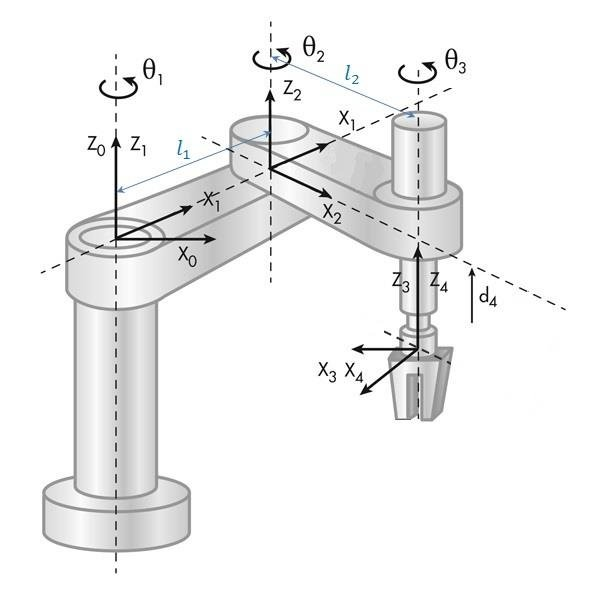
\includegraphics[width=0.25\textwidth]{Alan1.jpg}
        \caption{Modelo ilustrativo del robot SCARA}
    \end{figure}

    El modelo simplificado equivalente utilizado parte del eje de salida del tren de transmisión y toma en 
    cuenta la coordenada articular del eje de la articulación "hombro" denotada como $q_1(t) = θ_l(t)$. La 
    ecuación que describe este modelo es:

    \begin{equation}\label{eq:carga_mecanica1}
        J_{l}.\dot{\omega}_{l}(t) = T_{q}(t)-b_{l}.\omega_{l}(t)-T_{l}(t)
    \end{equation}

    \begin{equation}\label{eq:carga_mecanica2}
        \dot{\theta}_{l} = \omega_{l} \,\, \Leftrightarrow \,\, \theta_{l}(t) = \int_{0}^{t} \omega_{l}(\xi). \,d\xi + \theta_{l}(0)
    \end{equation}

    \noindent Parámetros equivalentes:\\

    \begin{tabular}{@{} p{0.35\textwidth} p{0.65\textwidth} @{}}
        \(\bullet\) Momento de inercia: & \(J_l \thickapprox (0.2520 \pm 0.1260) \, \text{kg.m}^2\) \\
        \(\bullet\) Amortiguamiento viscoso: & \(b_l \thickapprox (0 \pm 0.0030) \, \text{N.m.s/rad}\)
    \end{tabular}
    \\\\
    \noindent Especificaciones de operación:\\

    \begin{tabular}{@{} p{0.35\textwidth} p{0.65\textwidth} @{}}
        \(\bullet\) Torque de carga: & \(T_l(t) \thickapprox (0 \pm 6.28) \, \text{N.m}\)
    \end{tabular}
    

\subsection{Tren de transmisión}

    En este sistema, se utiliza una caja reductora reversible con un sistema de engranajes planetarios. Se 
    asume un acoplamiento rígido, lo que significa que no hay elasticidad torsional ni 
    juego o holgura en el sistema. El momento de inercia equivalente y las pérdidas de energía debidas a la 
    fricción interna se reflejan en el eje de entrada y se consideran junto con el motor.

    Al considerar este acoplamiento rígido, podemos simplificar el subsistema mecánico completo, ya que no 
    tenemos en cuenta la deformación elástica que ocurre en los engranajes durante la transmisión del par. 
    En otras palabras, podemos tratar la carga mecánica y el motor eléctrico como una unidad, lo que resulta 
    en un subsistema mecánico completo de un grado de libertad (1 g.d.l.).

    Las relaciones del modelo equivalente (rígido) del tren de transmisión son las siguientes:

    \begin{equation}\label{eq:tren_de_transmision1}
        \omega_{l}(t) = \frac{1}{r}.\omega_{m}(t)
    \end{equation}
    
    \begin{equation}\label{eq:tren_de_transmision2}
        T_{q}(t) = r.T_{d}(t)
    \end{equation}

    \noindent Parámetros equivalentes:\\

    \begin{tabular}{@{} p{0.35\textwidth} p{0.65\textwidth} @{}}
        \bullet\, Relación de reducción total: & \(r = 314.3008 : 1\)
    \end{tabular}
    \\\\
    Especificaciones de operación:\\

    \begin{tabular}{@{} p{0.35\textwidth} p{0.65\textwidth} @{}}
        \bullet\, Velocidad nominal (salida): \quad\quad\quad \ & \(n_{1nom} = 21 \, \text{rpm} \, (\omega_{lnom} = 2.2 \, \text{rad/s})\) \\
        \bullet\, Torque nominal: & \(T_{qnom}(t) = 7.26 \, \text{N.m}\) \\
        \bullet\, Torque pico: & \(T_{qmax}(t) = 29.42 \, \text{N.m}\)
    \end{tabular}


\subsection{Maquina eléctrica}
    
    En este caso, se utiliza un motor de corriente alterna (CA) trifásico con excitación por imanes permanentes. 

    \subsubsection{Subsistema mecánico}
        
        El subsistema mecánico del motor, que incluye el rotor y el tren de transmisión referidos 
        al estator estacionario, se describe mediante el siguiente modelo equivalente:
        
        \begin{equation}\label{eq:subsistema_macanico1}
            J_{m}.\dot{\omega}_{m}(t) = T_{m}(t)-b_{m}.\omega_{m}(t)-T_{d}(t)
        \end{equation}
        
        Además, se establece una relación entre la velocidad angular $\omega_m(t)$ y la derivada temporal de la 
        coordenada angular $\theta_m(t)$ mediante la relación:
        
        \begin{equation}\label{eq:subsistema_mecanico2}
            \dot{\theta}_{m} = \omega_{m} \Leftrightarrow \theta_{m}(t) = \int_{0}^{t} \omega_{m}(\xi). \,d\xi + \theta_{m}(0)
        \end{equation}

    \subsubsection{Subsistema electromagnético}
        
    En el caso de un motor eléctrico trifásico de tipo sincrónico con excitación por imanes permanentes, 
    es posible representar un modelo idealizado equivalente utilizando coordenadas eléctricas de 
    entrehierro $'qd0'$ fijas al rotor mediante la Transformación de Park del circuito del estator 
    estacionario.

    La Transformación de Park permite convertir el sistema de coordenadas trifásicas del estator 
    estacionario ($f_{abcs}(t)$) en coordenadas $'qd0'$ fijas al rotor ($f_{rqd0s}(t)$). Esto se hace 
    mediante la siguiente relación:

    \begin{equation}\label{eq:transformacion_de_park}
        \begin{bmatrix}
            f_{qs}^r(t)\\
            f_{ds}^r(t)\\
            f_{0s}^r(t)
        \end{bmatrix}
        =\frac{2}{3}.
        \begin{bmatrix}
            cos(\theta_r(t)) & cos(\theta_r(t) - \frac{2\pi}{3}) & cos(\theta_r(t) + \frac{2\pi}{3})\\
            sin(\theta_r(t)) & sin(\theta_r(t) - \frac{2\pi}{3}) & sin(\theta_r(t) + \frac{2\pi}{3})\\
            \frac{1}{2} & \frac{1}{2} & \frac{1}{2}
        \end{bmatrix}.
        \begin{bmatrix}
            f_{as}(t)\\
            f_{bs}(t)\\
            f_{cs}(t)
        \end{bmatrix}
    \end{equation}

    La transformación inversa, que nos permite volver al sistema de coordenadas del estator, se puede 
    expresar mediante la siguiente relación:
    
    \begin{equation}\label{eq:transformacion_de_park_inversa}
        \begin{bmatrix}
            f_{as}(t)\\
            f_{bs}(t)\\
            f_{cs}(t)
        \end{bmatrix}
        =
        \begin{bmatrix}
            cos(\theta_r(t)) & sin(\theta_r(t)) & 1\\
            cos(\theta_r(t) - \frac{2\pi}{3}) & sin(\theta_r(t) - \frac{2\pi}{3}) & 1\\
            cos(\theta_r(t) + \frac{2\pi}{3}) & sin(\theta_r(t) + \frac{2\pi}{3}) & 1
        \end{bmatrix}.
        \begin{bmatrix}
            f_{qs}^r(t)\\
            f_{ds}^r(t)\\
            f_{0s}^r(t)
        \end{bmatrix}
    \end{equation}

    Sabiendo qeu las coordenadas eléctrica del entrehierro $qd0$ fijas al rotor están dadas por:

    \begin{equation}\label{eq.coordenadas_fijas_al_rotor}
        \begin{aligned}
            \dot{\theta}_r = \omega_r(t) \Leftrightarrow  \theta_r = \int_0^t \omega_r(\xi).d\xi + \theta_r(0)\\
            \theta_r(t) = P_p.\theta_m(t) \therefore \omega_r(t) = P_p.\omega_m(t)\\
        \end{aligned}
    \end{equation}

    Se determina que el torque electromagnético se calcula utilizando la siguiente fórmula:

    \begin{equation}\label{eq.torque_electromagnetico}
        T_{m}(t) = \frac{3}{2}.P_{p}.[\lambda_{m}^{\prime r}+i_{ds}^r(t).(L_{d}-L_{q})].i_{qs}^r(t)
    \end{equation}
        
    \subsubsection{Subsistema térmico} 
    
    se consideran únicamente las pérdidas eléctricas resistivas debido al efecto Joule en el bobinado del 
    estator, sin tener en cuenta las pérdidas magnéticas en el núcleo. Además, se asume que la 
    transferencia de calor se produce por conducción y convección natural, sin utilizar ventilación forzada.

    La potencia de pérdidas calóricas se calcula utilizando las siguientes expresiones:

    \begin{equation}\label{termico1}
        P_{s_{perd}}(t) =  \frac{3}{2}.R_{s}(t).[i_{qs}^r(t)^2+i_{ds}^r(t)^2+2.i_{0s}(t)]\\
    \end{equation}
    
    \begin{equation}\label{termico2}
        P_{s_{perd}}(t) = C_{ts}.\dot{T}_{s}(t) + \frac{T_{s}(t)-T_{amb}(t)}{R_{ts-amb}}
    \end{equation}

    \noindent Parámetros equivalentes:\\

    \begin{tabular}{@{} p{0.4\textwidth} p{0.6\textwidth} @{}}
        \(\bullet\) Momento de inercia (motor y caja): & \(J_m \approx 3.1 \times 10^{-6} \, \text{kg.m}^2\) \\
        \(\bullet\) Coeficiente de fricción viscosa (motor y caja): & \(b_m \approx 1.5 \times 10^{-5} \, \text{N.m.rad/s}\) \\
        \(\bullet\) Pares de polos magnéticos: & \(P_p = 3\) pares (es decir, 6 polos) \\
        \(\bullet\) Flujo magnético equivalente de imanes concatenado por espiras del bobinado de estator: & \(\lambda'_{mr} \approx 0.01546 \, \text{V.s/rad}\)\\
        \(\bullet\) Inductancia de estator (eje en cuadratura): & \(L_q \approx 5.8 \, \text{mH}\) \\
        \(\bullet\) Inductancia de estator (eje directo): & \(L_d \approx 6.6 \, \text{mH}\) \\
        \(\bullet\) Inductancia de dispersión de estator: & \(L_{ls} \approx 0.8 \, \text{mH}\) \\
        \(\bullet\) Resistencia de estator, por fase: & \(R_s \approx 1.02 \, \Omega\) (@40 °C) → \(1.32 \, \Omega\) (@115 °C) \\
        \(\bullet\) Coeficiente de aumento de \(R_s\) con \(T_s^\circ(t)\): & \(\alpha_C = 3.9 \times 10^{-3} \, 1°C\) \\
        \(\bullet\) Capacitancia térmica de estator: & \(C_{ts} \approx 0.818 \, \text{W°C/s}\) (almacenamiento interno) \\
        \(\bullet\) Resistencia térmica estator-ambiente: & \(R_{ts-amb} \approx 146.7 \, °C/W\) (disipación al ambiente) \\
        \(\bullet\) Constante de tiempo térmica: & \(\tau_{ts-amb} = R_{ts-amb} \cdot C_{ts} \approx 120 \, \text{s}\)
    \end{tabular}    
    \\\\
    Especificaciones de operación:\\

    \begin{tabular}{@{} p{0.4\textwidth} p{0.6\textwidth} @{}}
        \(\bullet\) Velocidad nominal rotor: & \(n_m \approx 6600 \, \text{rpm}\) (\(\omega_m \approx 691.15 \, \text{rad/s}\)) \\
        \(\bullet\) Tensión nominal de línea: & \(V_{sl} \approx 24 \, \text{V}_{\text{ca rms}}\) (tensión nominal de fase: \(V_{sf} \approx V_{sl} \sqrt{3}\)) \\
        \(\bullet\) Corriente nominal: & \(I_s \approx 0.4 \, \text{A}_{\text{ca rms}}\) (régimen continuo) \\
        \(\bullet\) Corriente máxima: & \(I_{s \max} \approx 2.0 \, \text{A}_{\text{ca rms}}\) (corta duración, aceleración) \\
        \(\bullet\) Temperatura máxima de bobinado estator: & \(T_{s \max} = 115 \, °C\) \\
        \(\bullet\) Rango de temperatura ambiente de operación: & \(-15 °C \leq T_{amb} \leq 40 °C\)
    \end{tabular}

\subsection{Inversor trifásico de alimentación}

El sistema utiliza un inversor trifásico de 4 cuadrantes, compuesto por un puente trifásico con llaves 
electrónicas semiconductoras, como transistores MOSFETs o IGBTs, alimentado desde una fuente ideal de 
corriente continua (CC). El inversor se controla mediante modulación de ancho de pulso (PWM) y proporciona 
tensiones de fase equilibradas y senoidales en el estator de la máquina eléctrica sincrónica.

El modelo promediado considera las tensiones de fase en el estator como senoidales de secuencia positiva 
(abc) equilibradas, con un módulo variable Vsl(t) y una frecuencia ωe(t). El ángulo de carga del rotor, 
δ(t), representa el desfasaje instantáneo entre la coordenada eléctrica fija al rotor y la coordenada 
eléctrica sincrónica del estator, y depende del torque erogado.

\begin{figure}[H]
    \centering
    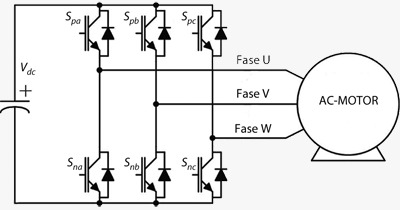
\includegraphics[width=0.5\textwidth]{Alan7.jpg}
    \caption{Circuito inversor ilustrativo}
\end{figure}

\subsection{Sensores de realimentación}

El sistema cuenta con varios dispositivos físicos para la medición y acondicionamiento de las variables. A 
continuación se describen los dispositivos y las variables medidas:

Un sensor de temperatura (por ejemplo, un sensor de resistencia térmica, RTD) ubicado en el bobinado del 
estator. La variable medida es $T_s(t)$, que se utiliza para monitorear el calentamiento y estimar la 
resistencia del estator, $R_s(t)$.

Sensor de posición angular (codificador incremental o "encoder") montado en el eje del motor. Se asume un 
proceso de "homing" y decodificación idealizada. La variable medida es $\theta_m(t)$, que representa la posición 
angular absoluta rectificada después de girar más de una revolución. 

  
Tres sensores de corriente instantánea de fase, montados en la salida trifásica del inversor hacia los 
bornes del estator. Las variables medidas son $i_{as}(t)$, $i_{bs}(t)$ y $i_{cs}(t)$, que representan las corrientes 
instantáneas de fase.

\begin{figure}[ht]
    \centering
    \begin{subfigure}[b]{0.3\textwidth}
      \centering
      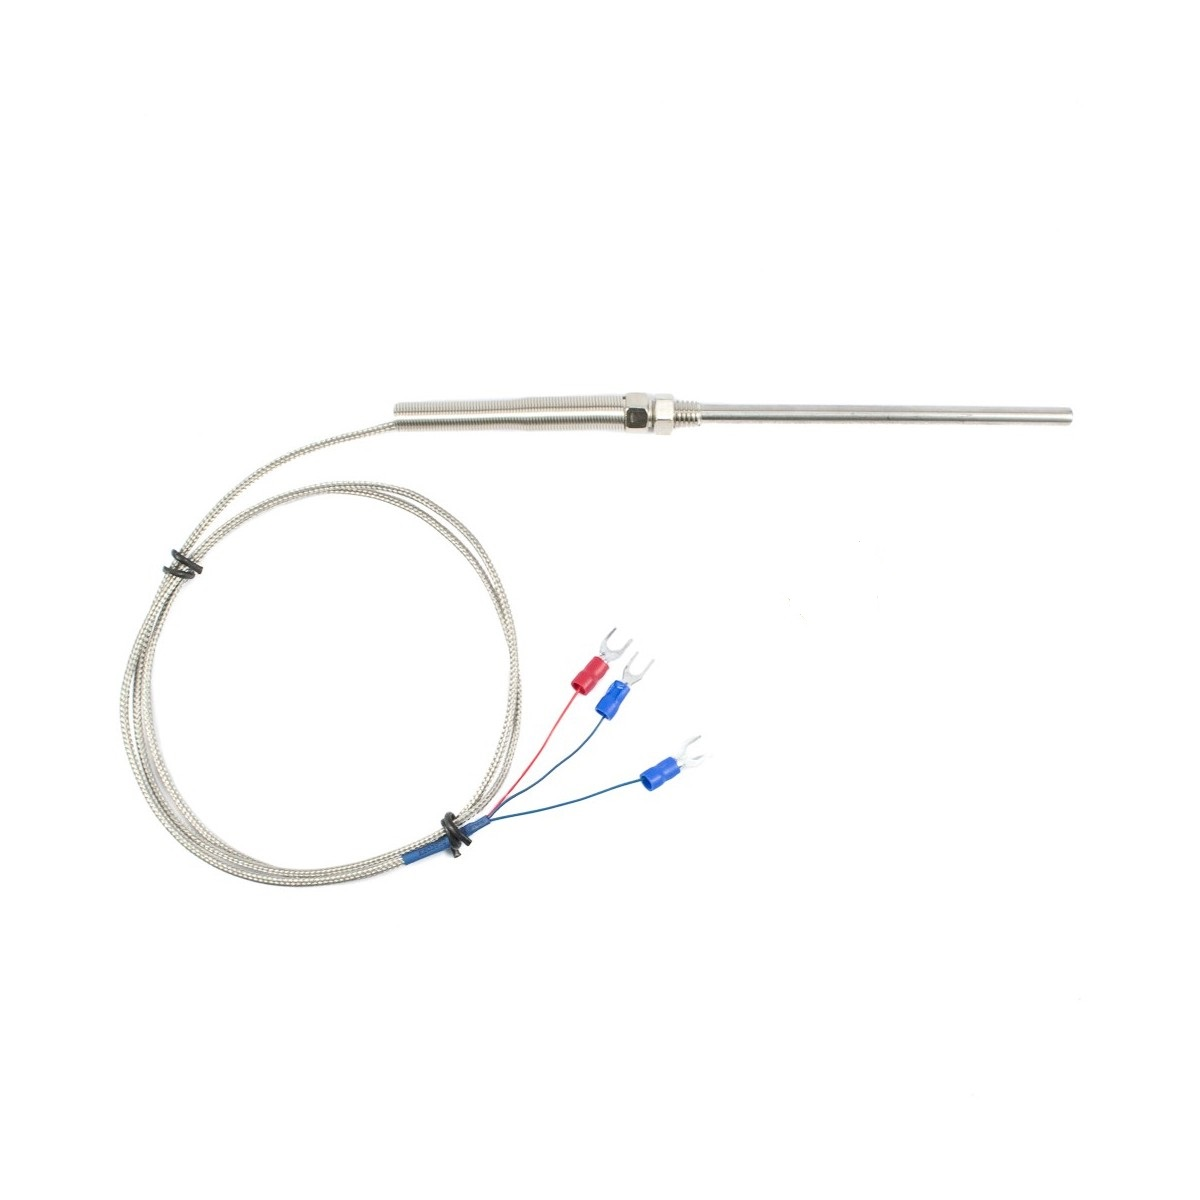
\includegraphics[width=0.75\textwidth]{Alan6.jpg}
      \caption{Sensor de temperatura}
    \end{subfigure}
    \begin{subfigure}[b]{0.3\textwidth}
      \centering
      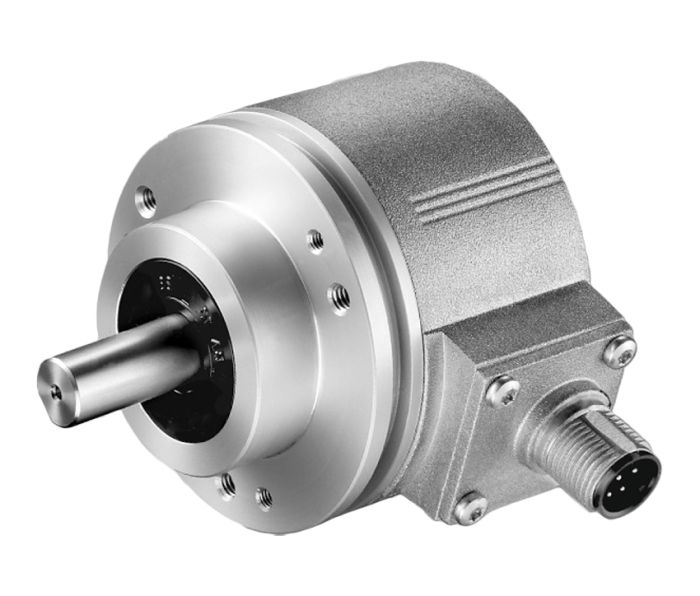
\includegraphics[width=0.75\textwidth]{Alan5.jpg}
      \caption{Encoder}
    \end{subfigure}
    \begin{subfigure}[b]{0.3\textwidth}
      \centering
      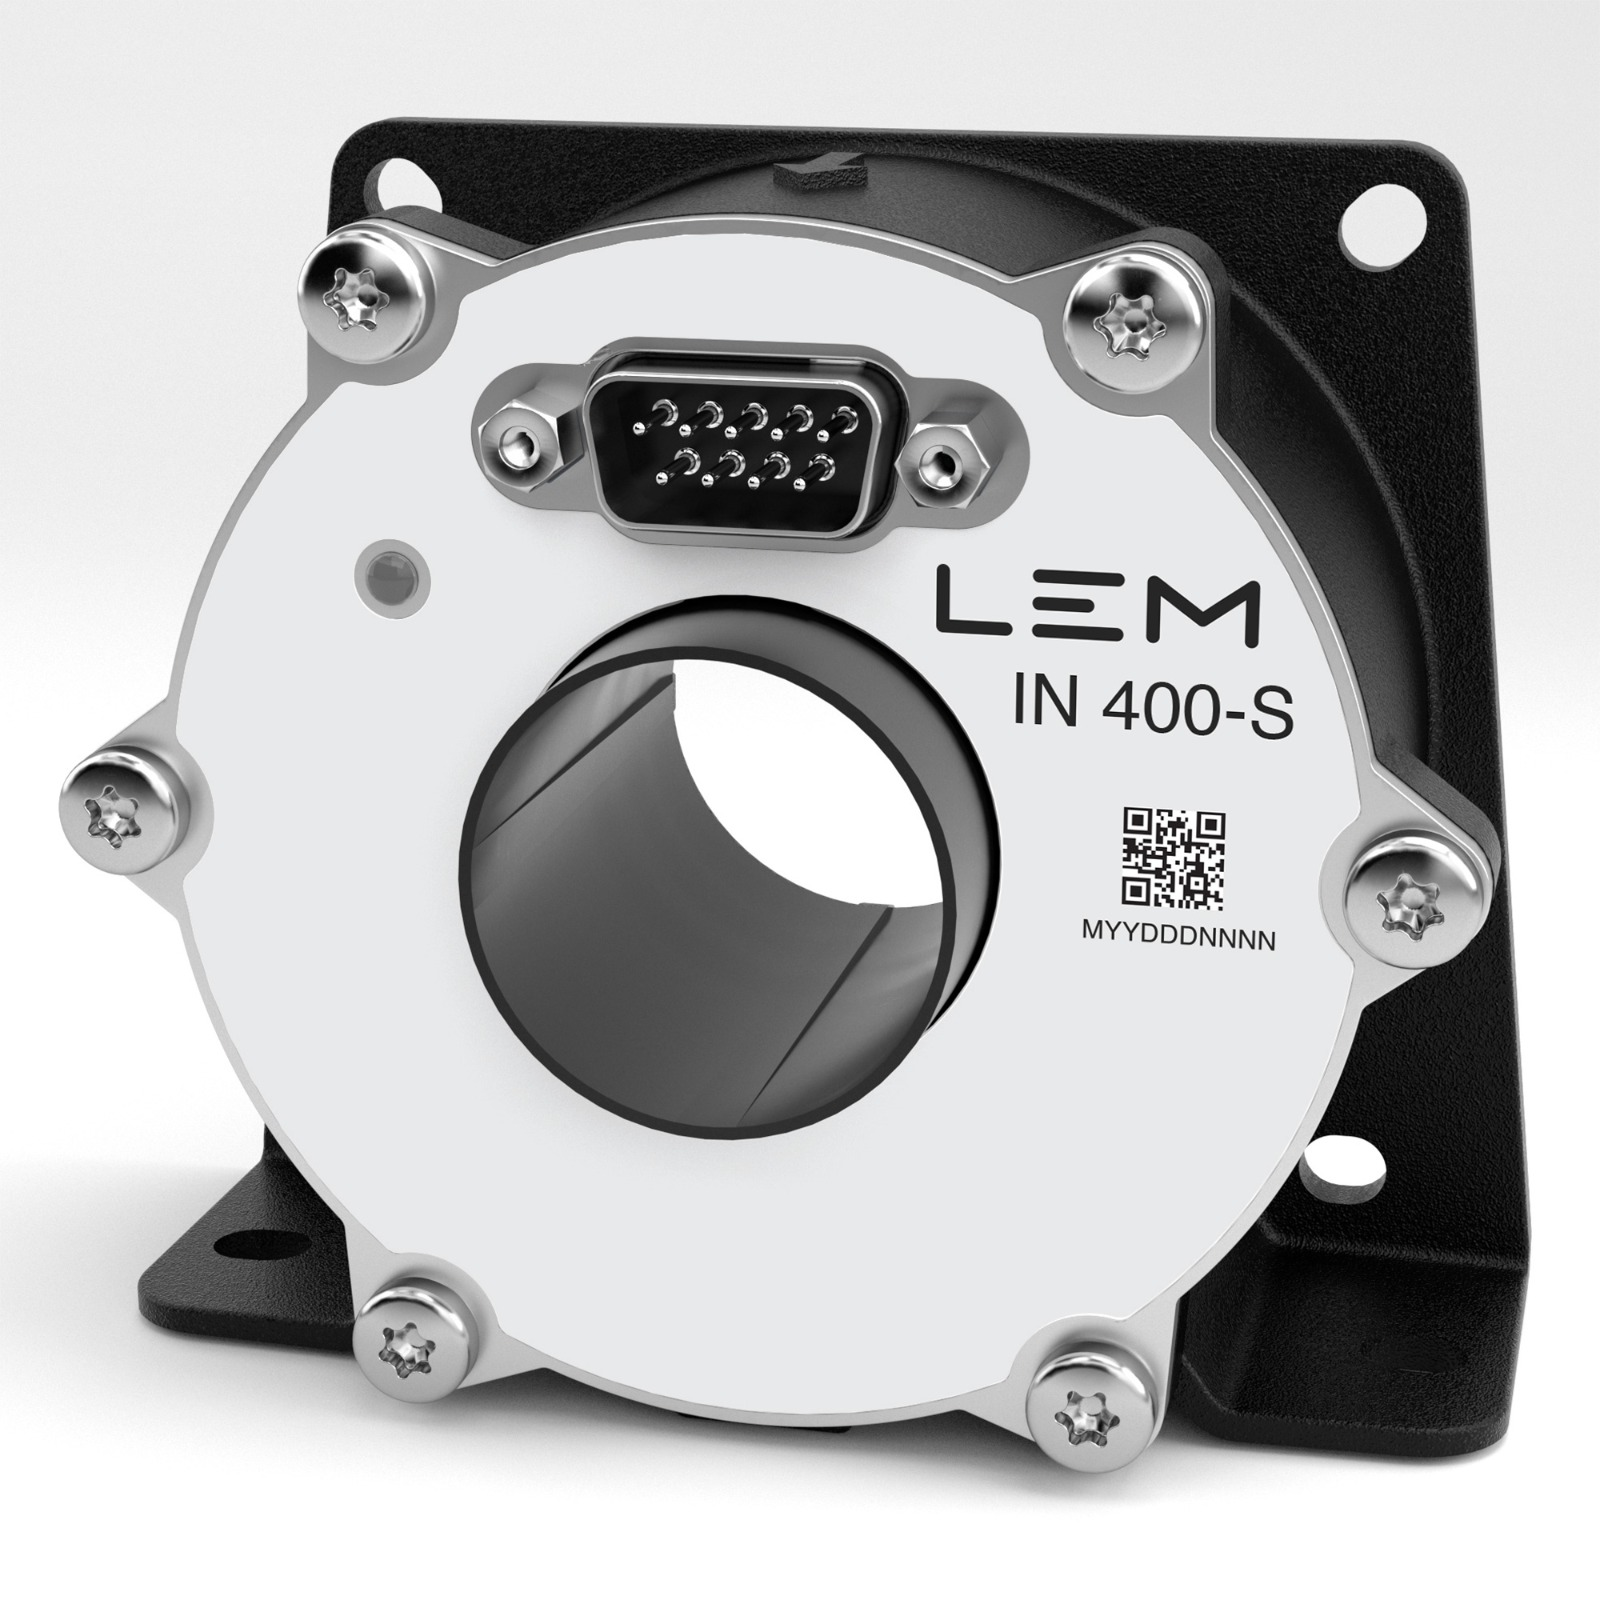
\includegraphics[width=0.75\textwidth]{Alan4.jpg}
      \caption{Sensor de corriente}
    \end{subfigure}
    \caption{Imágenes ilustrativas}
  \end{figure}


Se asume que todos los sensores tienen una respuesta ideal, es decir, un filtro "pasatodo" con ganancia 
unitaria y un ancho de banda infinito.

%-------------------------5.1-------------------------%

\section{Modelado, Análisis y Simulación dinámica del SISTEMA FÍSICO a Lazo Abierto}

%-------------------------5.1.1-------------------------%

\subsection{Modelo matemático equivalente del subsistema mecánico completo}

Para obtener el modelo matemático equivalente de un grado de libertad correspondiente al subsistema 
mecánico completo, primero debemos referenciar la carga al eje del rotor de la máquina eléctrica. Esto 
nos permitirá obtener un modelo matemático que tenga en cuenta la dinámica de la carga en relación con 
el rotor.

Comenzamos sustituyendo las ecuaciones de
\hyperref[eq:carga_mecanica1]{Carga mecánica (\ref*{eq:carga_mecanica1})}, 
\hyperref[eq:tren_de_transmision1, eq:tren_de_transmision2]{Tren de transmisión (\ref*{eq:tren_de_transmision1}, \ref*{eq:tren_de_transmision2})}, y
\hyperref[eq:subsistema_macanico1]{Subsistema mecánico (\ref*{eq:subsistema_macanico1})} de la maquina eléctrica.

\begin{equation}
    \label{eq:4.1}
    (J_{m}+\frac{J_l}{r^2}).\dot{\omega}_{m}(t) = T_{m}(t)-(b_{m}+\frac{b_{l}}{r^2}).\omega_{m}(t)-\frac{T_{l}(t)}{r} \\
\end{equation}

\begin{equation}
    J_{eq}.\dot{\omega}_{m}(t) = T_{m}(t)-b_{eq}.\omega_{m}(t)-\frac{T_{l}(t)}{r} \\
\end{equation}

\begin{equation}
    \dot{\omega}_{m}(t) = \frac{1}{J_{eq}}.[T_{m}(t) - b_{eq}.\omega_{m}(t) - \frac{T_{l}(t)}{r}]\\
\end{equation}

Se puede expresar de forma matricial como:

\begin{equation}
\begin{cases}
    \begin{bmatrix}
        \dot{\theta}_{m}(t)\\
        \dot{\omega}_{m}(t)\\
    \end{bmatrix}
    =
    \begin{bmatrix}
        0 & 1\\
        0 & -\frac{b_{eq}}{J_{eq}}\\
    \end{bmatrix}.
    \begin{bmatrix}
        \theta_{m}(t)\\
        \omega_{m}(t)\\
    \end{bmatrix}
    +
    \begin{bmatrix}
        0 & 0\\
        \frac{1}{J_{eq}} & -\frac{1}{J_{eq}r}\\
    \end{bmatrix}.
    \begin{bmatrix}
        T_{m}(t)\\
        T_{l}(t)\\
    \end{bmatrix}\\
    y(t) = 
    \begin{bmatrix} 1 & 0\\ \end{bmatrix} .
    \begin{bmatrix} \theta_{m}(t)\\ \omega_{m}(t)\\ \end{bmatrix}
\end{cases}
\end{equation}

Con este modelo matemático equivalente referido al eje del motor tiene como 
ventaja que no presenta backlash, ademas no hay que considerar el efecto de 
la elasticidad torsional de la transmisión.

% ------------------  5.1.2  --------------------- %

\subsection{Modelo dinámico del sistema físico completo}

% ------------------ 5.1.2.a --------------------- %

\subsubsection{Modelo global no lineal (NL)}

En el modelo global no lineal consideramos todos los sistemas involucrados 
tanto el sistema mecánico, previamente desarrollado, como los subsistemas de la maquina eléctrica.

En primer lugar, nos enfocaremos en el subsistema electromagnético, recordando que 
se utiliza un motor síncrono de corriente alterna (CA) trifásico con excitación de imanes 
permanentes. El estator esta conectado en estrella con bornes $abc$ accesible y neutro no accesible.
Consideramos que la carga de cada fase sera equivalente de forma que la conexión estrella este equilibrada.

Ecuaciones de tensión en coordenadas abc:

\begin{equation}\label{eq.tensiones_abc}
    \begin{aligned}
        v_{as}(t) &= R_{s}(t).i_{as}(t) + \frac{d\lambda_{as}}{dt}\\
        v_{bs}(t) &= R_{s}(t).i_{bs}(t) + \frac{d\lambda_{bs}}{dt}\\
        v_{cs}(t) &= R_{s}(t).i_{cs}(t) + \frac{d\lambda_{cs}}{dt}\\
    \end{aligned}
\end{equation}

Mediante la
\hyperref[eq:transformacion_de_park]{transformación de Park (\ref*{eq:transformacion_de_park})}
, se obtiene:

\begin{equation}\label{eq.tensiones_qd0}
    \begin{aligned}
        v_{qs}(t) &= R_{s}(t).i_{qs}(t) + L_{q}.\dot{i}_{qs}^r(t) + [\lambda_{m}^{\prime r} + L_{d}.i_{ds}(t)].\omega_{r}(t)\\
        v_{ds}(t) &= R_{s}(t).i_{ds}(t) + L_{d}.\dot{i}_{ds}^r(t)  - L_{q}.i_{qs}(t).\omega_{r}(t)\\
        v_{0s}(t) &= R_{s}(t).i_{0s}(t) + L_{ls}.\dot{i}_{0s}^r(t)
    \end{aligned}
\end{equation}

Reordenando nos quedan las ecuaciones que definen al sistema electromagnético:

\begin{equation}\label{eq:mi_ecuacion}
    \begin{cases}
        \dot{i}_{qs}(t) = \frac{1}{L_{q}}.[v_{qs}^r(t) - R_{s}(t).i_{qs}^r(t) - P_{p}.\omega_{m}(t).[L_{d}.i_{ds}^r(t) + \lambda_{m}^{\prime r}]]  \\
        \dot{i}_{ds}(t) = \frac{1}{L_{d}}.[v_{ds}^r(t) - R_{s}(t).i_{ds}^r(t) + P_{p}.\omega_{m}(t).L_{q}.i_{qs}^r(t)]  \\
        \dot{i}_{0s}(t) = \frac{1}{L_{ls}}.[v_{0s}^r(t) - R_{s}(t).i_{0s}^r(t)]
    \end{cases}
\end{equation}

Recordando que el
\hyperref[eq.torque_electromagnetico]{Torque electromagnético (\ref*{eq.torque_electromagnetico})} 
se reordena la expresión de forma que quede despejada la variable de interés:

\begin{equation}\label{eq.torque_electromagnetico_reordenado}
    \dot{\omega}_{m}(t) = \frac{1}{J_{eq}}.[\frac{3}{2}.P_{p}.[\lambda_{m}^{\prime r}+i_{ds}^r(t).(L_{d}-L_{q})].i_{qs}^r(t) - b_{eq}.\omega_{m}(t) - \frac{T_{l}(t)}{r}]\\
\end{equation}

El comportamiento subsistema térmico es descripto por las ecuaciones del
\hyperref[termico1, termico2]{(\ref*{termico1}, \ref*{termico2})}, igualando estas ecuaciones 
llegamos a la siguiente expresión:

\begin{equation}\label{termico3}
    \dot{T}_{s}(t) = \frac{1}{C_{ts}}.[\frac{3}{2}.R_{s}(t).[{i_{qs}^r(t)}^2+{i_{ds}^r(t)}^2 + 2.i_{0s}(t)^2] - \frac{T_{s}(t)-T_{amb}(t)}{R_{ts-amb}}]\\
\end{equation}

El modelo global no lineal queda definido por las ecuaciones (\ref{eq:subsistema_mecanico2}),
(\ref{eq:mi_ecuacion}), (\ref{eq.torque_electromagnetico_reordenado}) y (\ref{termico3}).

\begin{equation}\label{eq.modelo_global}
    \begin{cases}
        \dot{\theta}_{m}(t) = \omega_{m}(t)\\
        \dot{\omega}_{m}(t) = \frac{1}{J_{eq}}.[\frac{3}{2}.P_{p}.[\lambda_{m}^{\prime r}+i_{ds}^r(t).(L_{d}-L_{q})].i_{qs}^r(t) - b_{eq}.\omega_{m}(t) - \frac{T_{l}(t)}{r}]\\
        \dot{i}_{qs}(t) = \frac{1}{L_{q}}.[v_{qs}^r(t) - R_{s}(t).i_{qs}^r(t) - P_{p}.\omega_{m}(t).[L_{d}.i_{ds}^r(t) + \lambda_{m}^{\prime r}]]  \\
        \dot{i}_{ds}(t) = \frac{1}{L_{d}}.[v_{ds}^r(t) - R_{s}(t).i_{ds}^r(t) + P_{p}.\omega_{m}(t).L_{q}.i_{qs}^r(t)]  \\
        \dot{i}_{0s}(t) = \frac{1}{L_{ls}}.[v_{0s}^r(t) - R_{s}(t).i_{0s}^r(t)]\\
        \dot{T}_{s}(t) = \frac{1}{C_{ts}}.[\frac{3}{2}.R_{s}(t).[{i_{qs}^r(t)}^2+{i_{ds}^r(t)}^2 + 2.i_{0s}(t)^2] - \frac{T_{s}(t)-T_{amb}(t)}{R_{ts-amb}}]\\
    \end{cases}
\end{equation}

De este sistema podemos definir el vector de las variables de estado, las entradas 
manipuladas, las entradas de perturbación y las salidas:

\[ x(t) =
\begin{bmatrix}
\theta_m(t) \\
\omega_m(t) \\
i^r_{qs}(t) \\
i^r_{ds}(t) \\
i_{0s}(t) \\
T_s(t)
\end{bmatrix}
; \quad
x(t_0) =
\begin{bmatrix}
\theta_{m0} \\
\omega_{m0} \\
i^{r0}_{qs} \\
i^{r0}_{ds} \\
i_{0s0} \\
T_{s0}
\end{bmatrix}
; \quad
u(t) =
\begin{bmatrix}
v^r_{qs}(t) \\
v^r_{ds}(t) \\
v_{0s}(t)
\end{bmatrix}
; \quad
d(t) =
\begin{bmatrix}
T_l(t) \\
T_{\text{amb}}(t)
\end{bmatrix}
; \quad
y(t) = 
\begin{bmatrix}
    \theta_m(t) \\
    \omega_m(t) \\
    i^r_{qs}(t) \\
    i^r_{ds}(t) \\
    i_{0s}(t) \\
    T_s(t)
\end{bmatrix}
\]

% Imagen del modelo global no lineal

Utilizando las ecuaciones que modelan las distintas partes del sistema realizamos el 
diagrama de bloques utilizando la herramienta que nos provee Matlab, Simulink.

\begin{figure}[H]
    \centering
    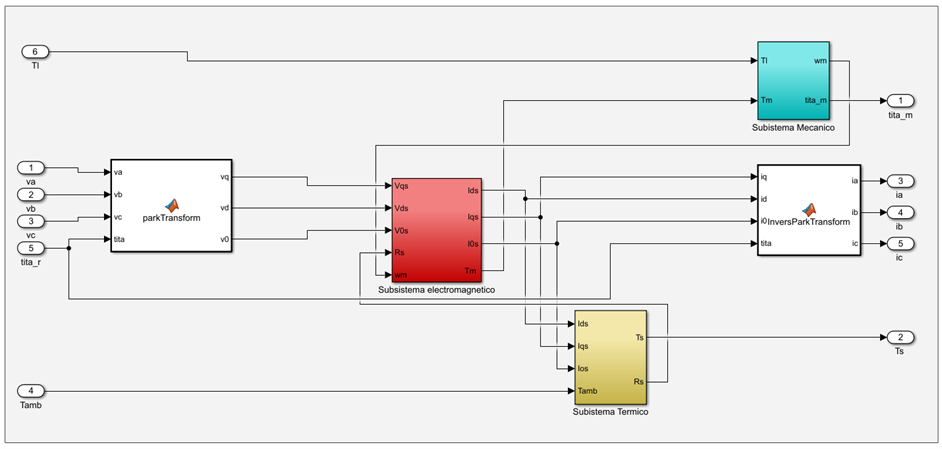
\includegraphics[width=1\textwidth]{no_lineal.png}
    \caption{Modelo global no lineal}
\end{figure}

El subsistema mecánico esta compuesto por:

\begin{figure}[H]
    \centering
    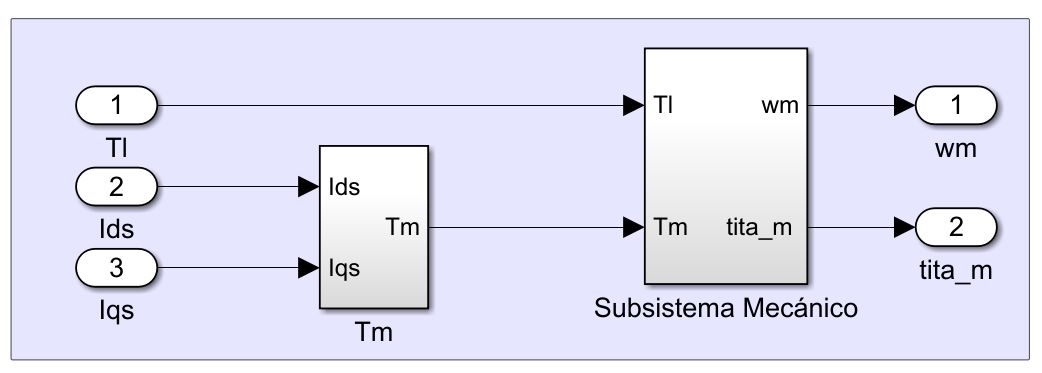
\includegraphics[width=1\textwidth]{sub_mecanico.png}
    \caption{Diagramas de bloques subsistema mecánico}
\end{figure}

Donde los bloques interno son:

\begin{figure}[H]
    \begin{subfigure}[b]{0.5\textwidth}
        \centering
        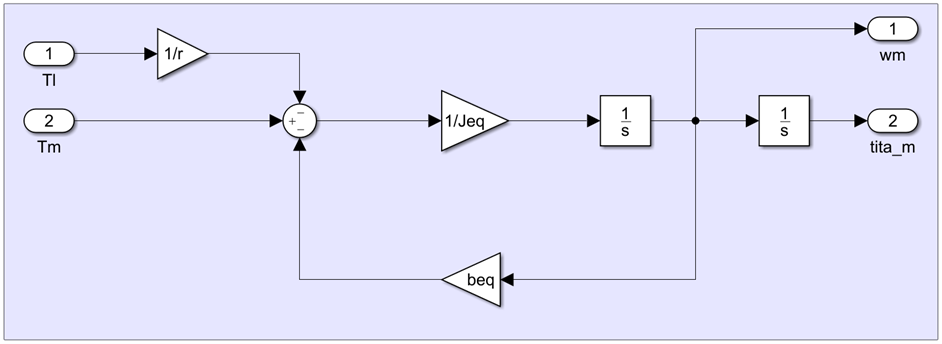
\includegraphics[width=1\textwidth]{sub_mecanico2.png}
    \end{subfigure}
    \begin{subfigure}[b]{0.5\textwidth}
        \centering
        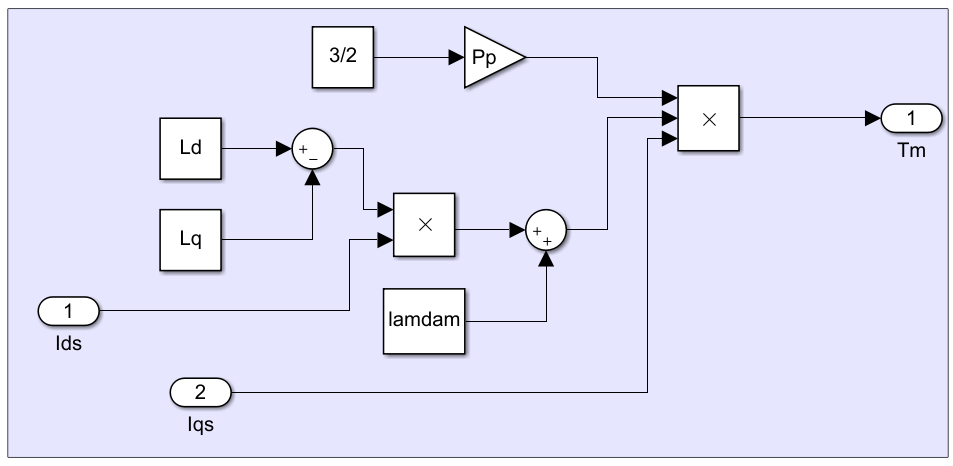
\includegraphics[width=1\textwidth]{sub_mecanico3.png}
    \end{subfigure}
    \caption{Bloques internos del subsistema mecánico}
\end{figure}

Mientras que el subsistema térmico esta dado por:

\begin{figure}[H]
    \centering
    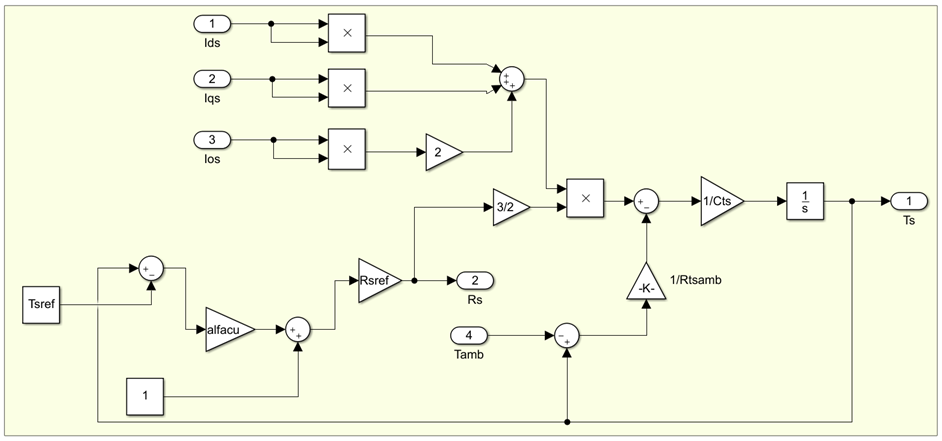
\includegraphics[width=1\textwidth]{sub_termico.png}
    \caption{Diagramas de bloques subsistema térmico}
\end{figure}

Finalmente el subsistema electromagnético esta compuesto por:

\begin{figure}[H]
    \centering
    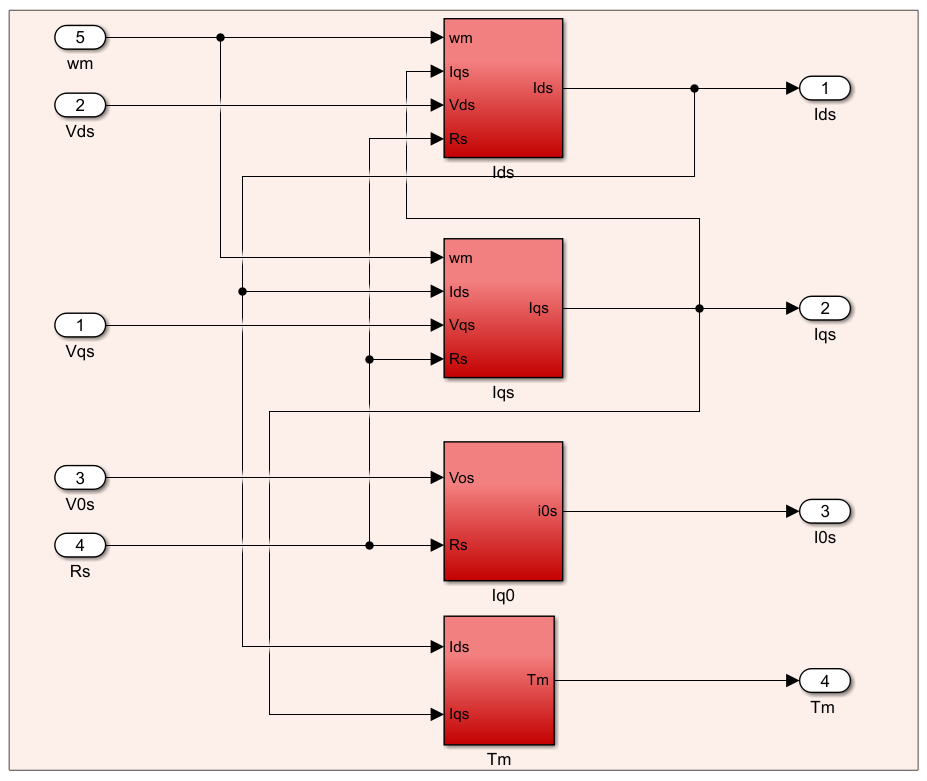
\includegraphics[width=1\textwidth]{sub_electromagentico.png}
\end{figure}

Los bloques interno contienen:

\begin{figure}[H]
    \centering
    \begin{subfigure}[]{1\textwidth}
        \centering
        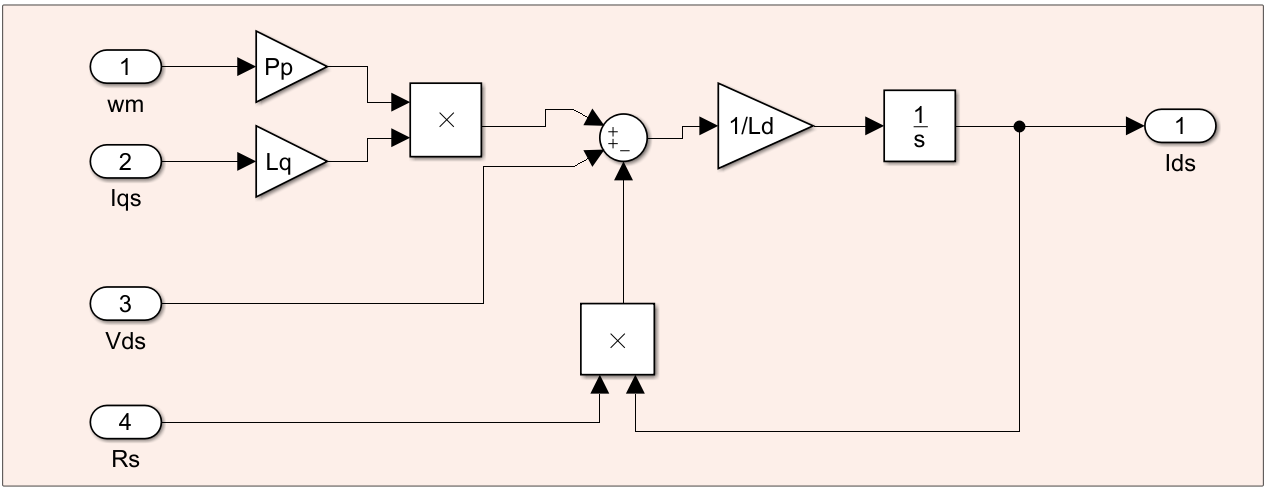
\includegraphics[width=1\textwidth]{sub_electromagentico4.png}
    \end{subfigure}
    \\
    \begin{subfigure}[b]{1\textwidth}
        \centering
        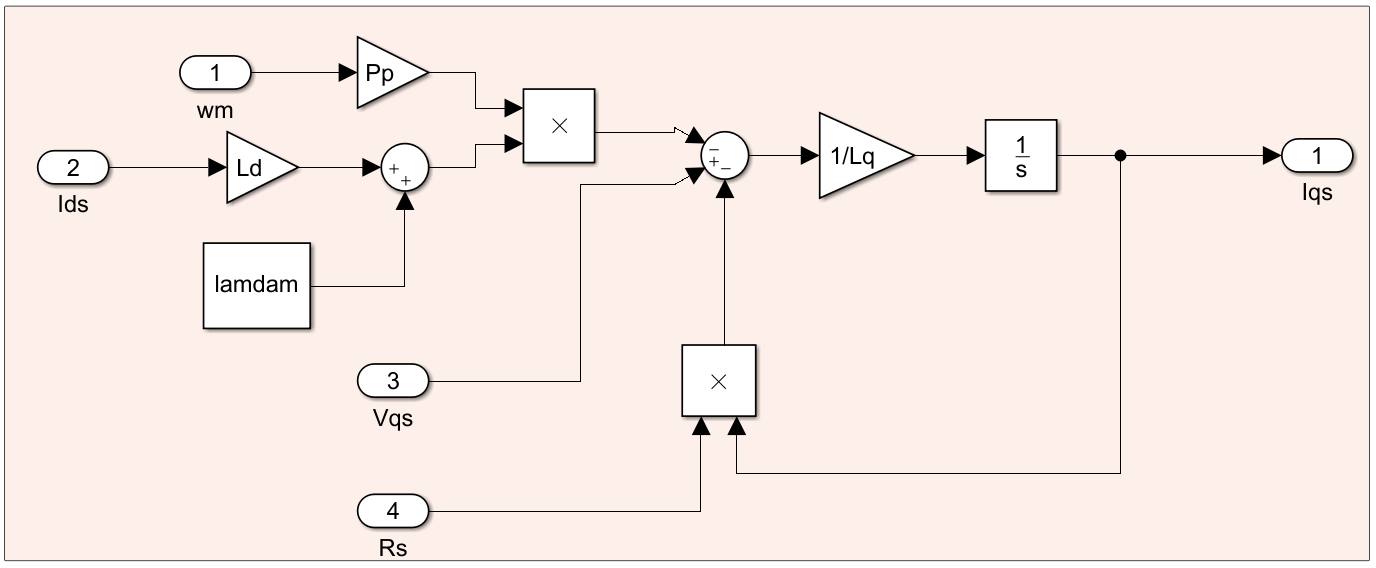
\includegraphics[width=1\textwidth]{sub_electromagentico3.png}
    \end{subfigure}
    \\
    \begin{subfigure}[b]{1\textwidth}
        \centering
        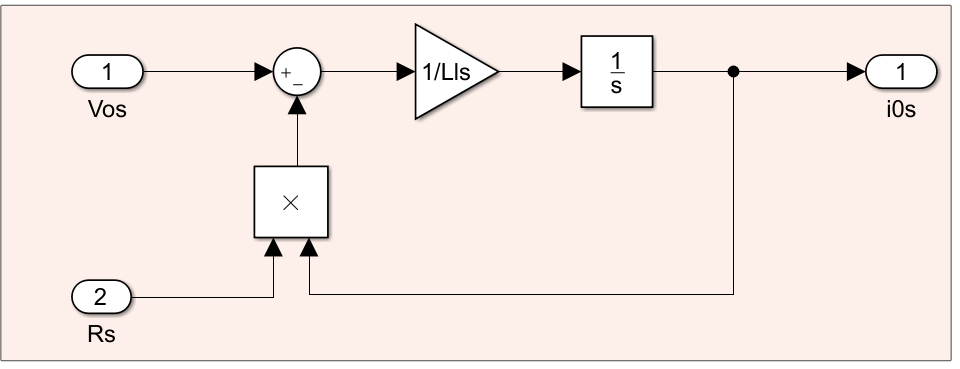
\includegraphics[width=1\textwidth]{sub_electromagentico2.png}
    \end{subfigure}
    \caption{Bloques internos del subsistema electromagnético}
\end{figure}

%-------------------------- 5.1.2.B ------------------------------------------%

\subsubsection{Modelo global linealizado con parámetros variables (LPV)}

Para el caso general en el que ${i}_{ds}(t) \neq 0$. Se puede representar al sistema no lineal de forma genérica
como: 

\begin{equation}
    \begin{cases}
        \dot{x}(t) = f(x(t),u(t));  \quad   x(t_{0}) = x_{0}\\
        y(t) = C.x(t)\\
    \end{cases}
\end{equation}

Donde $f$ es una función que representa la dinámica del sistema en términos de las variable 
de estado $x(t)$ y las estradas $u(t)$.  
Dados los punto de equilibrio dinámico donde las derivadas de las variables de estado son nulas:

\begin{equation}
    \dot{x}(t) = f(x(t),u(t)) = 0
\end{equation}

Todos los pares de puntos $[X_0,U_0]$ que satisfacen la ecuación anterior definen el conjunto de
puntos de operación. Estos puntos los consideraremos cuasi-estacionarios. 

Alrededor de estos puntos consideraremos pequeñas variaciones infinitesimales:

\begin{equation}
    \begin{cases}
        x(t) = X_{0}(t) + \Delta x(t)\\
        u(t) = U_{0}(t) + \Delta u(t)\\
        y(t) = Y_{0}(t) + \Delta y(t)\\
    \end{cases}
\end{equation}

De forma que el el sistema genérico global NL queda representado por:

\begin{equation}
    \begin{cases}
        \dot{x}(t) = \dot{X}_{0}(t) + \Delta\dot{x}(t) = f(X_{0}(t) + \Delta x(t), U_{0}(t) + \Delta u(t))\\
        X_{0}(0) + \Delta x(0) = x_{0} \quad\quad\quad \rightarrow \quad X_{0} = x_{0}, \Delta x(0) = 0 \\
        Y_{0}(t) + \Delta y(t) = C(X_{0}(t) + \Delta x(t)) \quad\rightarrow\quad Y_{0}(t) = C X_{0}(t); \Delta y(t) = C \Delta x(t)\\
    \end{cases}
\end{equation}

Aproximación mediante la serie de Taylor truncada al primer orden y despreciando los terminos
de orden superior:

\begin{equation}
    f(X_{0}(t) + \Delta x(t), U_{0}(t) + \Delta u (t)) \approx f(X_{0}(t), U_{0}(t)) + \frac{\partial f}{\partial x}\mid_{0}\Delta x(t) + \frac{\partial f}{\partial u}\mid_{0}\Delta u(t)
\end{equation}

Al aplicar esto a nuestro modelo NL el sistema se divide en dos partes, una NL cuasi-estacionaria y otra 
lineal dinámica que representa las pequeñas variaciones alrededor de puntos de operación.

Modelo NL cuasi-estacionario:

\begin{equation}
    \dot{X}_{0}(t) = f(X_{0}(t), U_{0}(t)) \quad \approx 0 \;/\; \text{cte}; \quad X_{0}(0) = x_{0}
\end{equation}

Modelo lineal dinámico:

\begin{equation}
    \Delta\dot{x}(t) = \frac{\partial f}{\partial x}\mid_{0}\Delta x(t) + \frac{\partial f}{\partial u}\mid_{0}\Delta u(t); \quad \Delta x(0) = 0\\
\end{equation}

Al aplicar este concepto a las ecuaciones del
\hyperref[eq.modelo_global]{Modelo global NL (\ref*{eq.modelo_global})}
obtenemos:

\begin{itemize}

    \item Espacio de operación global NL (cuasi - estacionario)

    \begin{equation}
        \begin{cases}
            \dot{\theta}_{m0} = \omega_{m0} = cte\\
            \dot{\omega}_{m0} = \frac{1}{J_{eq}}.[\frac{3}{2}.P_{p}.[\lambda_{m}^{\prime r} + i_{ds0}^r.(L_{d}-L_{q})].i_{qs0}^r - b_{eq}.\omega_{m0} - \frac{T_{l0}}{r}] = 0\\
            \dot{i}_{qs0} = \frac{1}{L_{q}.}[v_{qs0}^r - R_{s}(t).i_{qs0}^r - P_{p}.\omega_{m0}.[L_{d}.i_{ds0}^r + \lambda_{m}^{\prime r}]] = 0\\
            \dot{i}_{ds0} = \frac{1}{L_{d}}.[v_{ds0}^r - R_{s}(t).i_{ds0}^r + P_{p}.\omega_{m0}.L_{q}.i_{qs0}^r] = 0 \\
            \dot{i}_{0s0} = \frac{1}{L_{ls}}.[v_{0s0}- R_{s}(t).i_{0s0}] = 0\\
            \dot{T}_{s0} = \frac{1}{C_{ts}}.[\frac{3}{2}.R_{s}(t).[{i_{qs0}^r}^2 + {i_{ds0}^r}^2 + 2.i_{0s0}^2]-\frac{T_{s0}-T_{amb0}}{R_{ts-amb}}] = 0\\
        \end{cases}
    \end{equation}

    \item Modelo dinámico LPV
    \begin{equation}
        \begin{cases}
            \Delta\dot{\theta}_{m}(t) = \Delta\omega_{m}(t)\\
            \Delta\dot{\omega}_{m}(t) = \frac{1}{J_{eq}}.[\frac{3}{2}.P_{p}.\{[\lambda_{m}^{\prime r} + i_{ds0}^r.(L_{d}-L_{q})].\Delta i_{qs}^r(t) + \Delta i_{ds}^r(t).(L_{d}-L_{q})].i_{qs0}^r\}- b_{eq}.\Delta\omega_{m}(t) - \frac{\Delta T_{l}(t)}{r}]\\
            \Delta\dot{i}_{qs}(t) = \frac{1}{L_{q}}.[\Delta v_{qs}^r(t) - R_{s}(t).\Delta i_{qs}^r(t) - P_{p}.\Delta\omega_{m}(t).[L_{d}.i_{ds0}^r + \lambda_{m}^{\prime r}] - P_{p}.\omega_{m0}.L_{d}.\Delta i_{ds}^r(t)] \\
            \Delta\dot{i}_{ds}(t) = \frac{1}{L_{d}}.\Delta [v_{ds}^r(t) - R_{s}(t).\Delta i_{ds}^r(t) + P_{p}.\Delta\omega_{m}(t).L_{q}.i_{qs0}^r + P_{p}.\omega_{m0}.L_{q}.\Delta i_{qs}^r(t)]  \\
            \Delta\dot{i}_{0s}(t) = \frac{1}{L_{ls}}.[\Delta v_{0s}(t) - R_{s}(t).\Delta i_{0s}(t)] \\
            \Delta\dot{T}_{s}(t) = \frac{1}{C_{ts}}.\{\frac{3}{2}.R_{s}(t).[{2.i_{qs}^r.\Delta i_{ds}^r(t)} + 2.i_{as}^r.\Delta i_{as}^r(t) + 4.i_{0s}.\Delta i_{0s}(t)]-\frac{\Delta T_{s}(t)-\Delta T_{amb}(t)}{R_{ts-amb}}\}\\
        \end{cases}
    \end{equation}

    En forma matricial:

\begin{equation*}
\begin{gathered}
    \begin{bmatrix}
        \Delta\dot{\theta}_{m}(t)\\
        \Delta\dot{\omega}_{m}(t)\\
        \Delta\dot{i}_{qs}(t)\\
        \Delta\dot{i}_{ds}(t)\\
        \Delta\dot{i}_{0s}(t)\\
        \Delta\dot{T}_{s}(t)\\
    \end{bmatrix} =
    \begin{bmatrix}
        0 & 1 & 0 & 0 & 0  & 0 \\
        0 & -b_{eq} & \frac{3}{2}.P_{p}.\frac{[\lambda_{m}^{\prime r} + i_{qs0}^r(t).(L_{d}-L_{q})]}{J_{eq}} & \frac{3}{2}.\frac{P_{p}.(L_{d}-L_{q}).i_{qs}^r}{J_{eq}} & 0 & 0\\
        0 & -\frac{P_{p}.(\lambda_{m}^{\prime r} + L_{d}.i_{ds0}^r)}{L_{q}} & -\frac{R_{s}(t)}{L_{q}} & -\frac{L_{d}.P_{p}.\omega_{m0}}{L_{q}} & 0 & 0\\
        0 & \frac{P_{p}.i_{qs0}^r .L_{q}}{L_{d}} & \frac{L_{q}.P_{p}.\omega_{m0}}{L_{d}} & -\frac{R_{s}(t)}{L_{d}} & 0 & 0\\
        0 & 0 & 0 & 0 & -\frac{R_{s}(t)}{L_{ls}} & 0\\
        0 & 0 & \frac{3.R_{s}(t)}{C_{ts}}.i_{qs0}^r & \frac{3.R_{s}(t)}{C_{ts}}.i_{ds0}^r & \frac{6.R_{s}(t)}{C_{ts}}.i_{0s0} & -\frac{1}{C_{ts}.R_{ts-amb}}\\
    \end{bmatrix}.\\
    \begin{bmatrix}
        \Delta{\theta}_{m}(t)\\
        \Delta{\omega}_{m}(t)\\
        \Delta{i}_{qs}(t)\\
        \Delta{i}_{ds}(t)\\
        \Delta{i}_{0s}(t)\\
        \Delta{T}_{s}(t)\\
    \end{bmatrix}  + 
    \begin{bmatrix}
        0 & 0 & 0 & 0 & 0\\
        -\frac{1}{rJ_{eq}} & 0 & 0 & 0 & 0\\
        0 & \frac{1}{L_{q}} & 0 & 0 & 0\\
        0 & 0 & \frac{1}{L_{d}} & 0 & 0\\
        0 & 0 & 0 & \frac{1}{L_{ls}} & 0\\
        0 & 0 & 0 & 0 & \frac{1}{C_{ts}R_{ts-amb}}\\
    \end{bmatrix}
    \begin{bmatrix}
        \Delta{T}_{l}(t)\\
        \Delta{V}_{qs}(t)\\
        \Delta{V}_{ds}(t)\\
        \Delta{V}_{0s}(t)\\
        \Delta T_{amb}(t)\\
    \end{bmatrix} 
\end{gathered}
\end{equation*}

\end{itemize}

%-------------------- 5.1.2.c --------------------------%

\subsubsection{Linealización por Realimentación NL}

Podemos obtener un modelo simplificado lineal invariante en el tiempo (LTI) equivalente del sistema
si aplicamos una estrategia de control vectorial con campo orientado en el controlador para imponer
que la corriente en el eje d $i_{ds}(t)$ sea igual a cero. Además, podemos despreciar 
el acoplamiento no lineal con el subsistema térmico debido a las pequeñas variaciones de la 
resistencia \(R_s\) con la temperatura, lo que nos permite considerar su dinámica como lineal.

Considerando que el estator de la máquina eléctrica es de tipo estrella con neutro flotante, 
podemos afirmar que la suma de las corrientes de fase \(abc\) será nula. Con esto, podemos aplicar 
una transformación directa de Park para relacionar las corrientes en el sistema.

Para lograr la desacoplar los canales de flujo magnético y torque, aplicamos la estrategia de 
"Control Vectorial con campo orientado." Esto consiste en forzar una corriente nula en el eje 
d \(i_{ds}(t) = 0\) mediante el controlador y, si es necesario, aplicar una "Restricción o Ley 
de Control NL" sobre la variable manipulada virtual \(v_{qd0s}(t)\) o su equivalente por 
transformada de Park, \(v_{{abc}}(t)\).

Para desacoplar el subsistema térmico, consideramos que las variaciones en la resistencia \(R_s\) 
en el rango de temperaturas de trabajo son despreciables y, por lo tanto, la temperatura no 
afectará significativamente el comportamiento del resto del sistema. Esto nos permite asumir 
una dinámica lineal para el subsistema térmico.

\begin{enumerate}[label=\roman*.]
    \item \textbf{Ecuaciones vectoriales/matriciales LTI de estado y de salida.} 
    
    Aplicadas las condiciones mencionadas nos queda un sistema LTI similar al de un maquina 
    de corriente continua con escobillas. El estado inicial sera nulo.

    \begin{equation}\label{eq.lti}
        \begin{cases}
            \dot{\theta}_{m}(t) = \omega_{m}(t)\\
            \dot{\omega}_{m}(t) = \frac{1}{J_{eq}}[\frac{3}{2}P_{p}\lambda_{m}^{\prime r}i_{qs}^r(t) - b_{eq}\omega_{m}(t) - \frac{T_{l}(t)}{r}]\\
            \dot{i}_{qs}(t) = \frac{1}{L_{q}}[v_{qs}^r(t) - R_{s}i_{qs}^r(t) - P_{p}\omega_{m}(t)\lambda_{m}^{\prime r}]  \\
        \end{cases}
    \end{equation}

    De forma matricial:

    \begin{equation}
        \begin{cases}
            \begin{bmatrix}
                \dot{\theta}_{m}(t)\\
                \dot{\omega}_{m}(t)\\
                \dot{i}_{qs}(t)\\
            \end{bmatrix} =
            \begin{bmatrix}
                0 & 1 & 0\\
                0 & -\frac{b_{eq}}{J_{eq}} & \frac{3}{2}\frac{P_{p}\lambda_{m}^{\prime r}}{J_{eq}}\\
                0 & -\frac{P_{p}\lambda_{m}^{\prime r}}{L_{q}} & -\frac{R_{s}}{L_{q}}\\
            \end{bmatrix}
            \begin{bmatrix}
                {\theta}_{m}(t)\\
                {\omega}_{m}(t)\\
                {i}_{qs}(t)\\
            \end{bmatrix} +
            \begin{bmatrix}
                0\\
                0\\
                \frac{1}{L_{eq}}\\
            \end{bmatrix} v_{qs}^r(t) +
            \begin{bmatrix}
                0\\
                -\frac{1}{rJ_{eq}}\\
            \end{bmatrix} T_{l}(t)\\
            y(t) =
            \begin{bmatrix}
                1 & 0 & 0\\
            \end{bmatrix}
            \begin{bmatrix}
                {\theta}_{m}(t)\\
                {\omega}_{m}(t)\\
                {i}_{qs}(t)\\
            \end{bmatrix}
        \end{cases}
    \end{equation}

    Para linealizar el subsistema térmico podemos suponer que $R_s$ sera constante debido a su poca variación
    de forma que:

    \begin{equation}
        \dot{T}_{s}(t) = \frac{1}{C_{ts}}.[\frac{3}{2}.R_{s}.{i_{qs}^r(t)}^2 - \frac{T_{s}(t)-T_{amb}(t)}{R_{ts-amb}}]\\
    \end{equation}
        
    \item \textbf{Diagrama de bloques de estado}
    
    \begin{figure}[H]
        \centering
        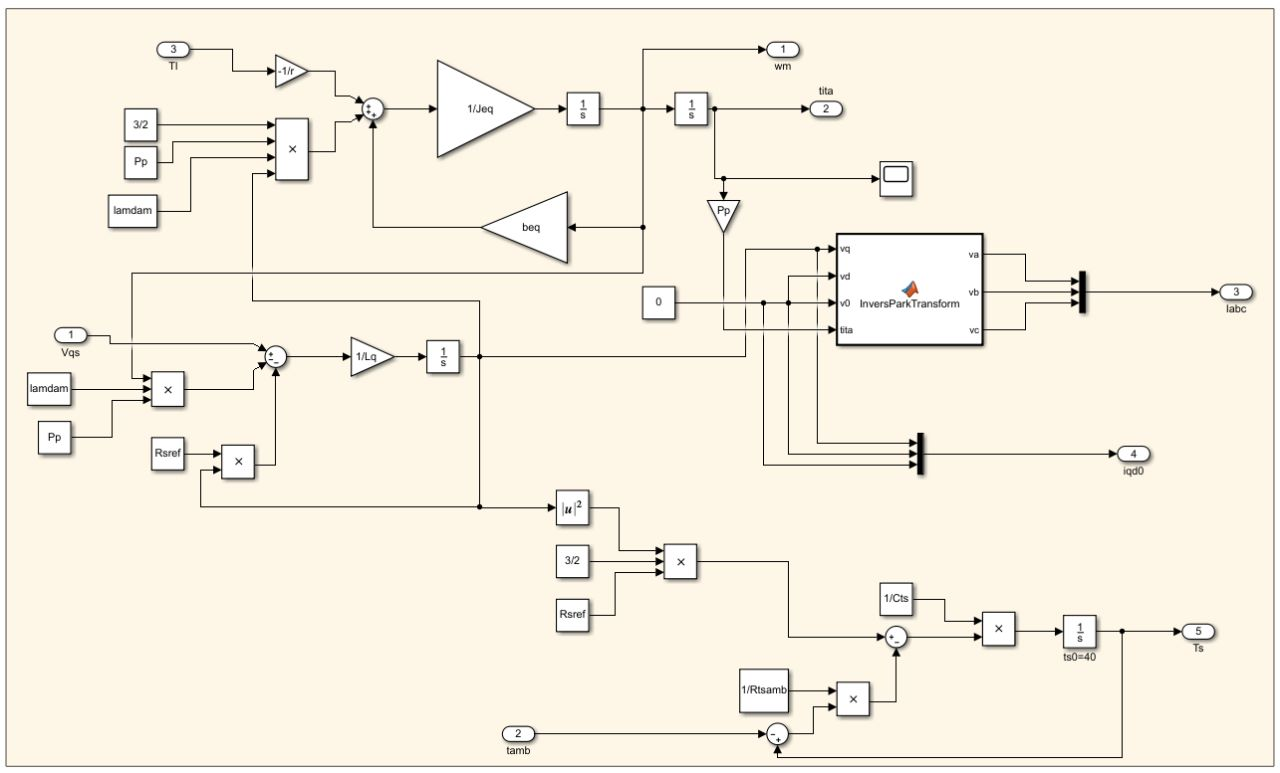
\includegraphics[width=1\textwidth]{LTI.png}
        \caption{Diagrama de bloques de estado del sistema LTI.}
    \end{figure}
    
    \item \textbf{Restricción o Ley de Control mínima}

    Para poder cumplir con la restricción de $i_{ds} = 0$ se tiene que cumplir la condición dada por la
    \hyperref[eq.tensiones_qd0]{ecuación (\ref*{eq.tensiones_qd0})}. De manera que:

    \begin{equation}
        v_{ds}^r(t) = -L_{q}.i{qs}^r(t).\omega_{m}(t).P_{p}
    \end{equation}

    Dado que se trata de una variable virtual no podemos controlarla directamente, por lo que buscaremos
    expresarla en termino de las coordenadas "abc", por lo que aplicamos la transformada inversa de Park.
    Resolviendo llegamos a:

    \begin{equation}
        \begin{cases}
            v_{as}(t) = cos(\theta_{r}(t)).v_{qs}^r(t) + sin(\theta_{r}(t)).v_{ds}^r(t) + v_{0s}^r(t)\\
            v_{bs}(t) = cos(\theta_{r}(t) - \frac{2\pi}{3}).v_{qs}^r(t) + sin(\theta_{r}(t) - \frac{2\pi}{3}).v_{ds}^r(t) + v_{0s}^r(t)\\
            v_{cs}(t) = cos(\theta_{r}(t) + \frac{2\pi}{3}).v_{qs}^r(t) + sin(\theta_{r}(t) + \frac{2\pi}{3}).v_{ds}^r(t) + v_{0s}^r(t)\\
        \end{cases}
    \end{equation}

    Dado que los valores de $v_{ds}(t)$ y $v_{0s}(t)$ son conocidos los sustituimos: 

    \begin{equation}
        \begin{cases}
            v_{as}(t) = cos(\theta_{r}(t))v_{qs}^r(t) - sin(\theta_{r}(t))L_{q}i{qs}^r(t)\omega_{m}(t)P_{p}\\
            v_{bs}(t) = cos(\theta_{r}(t) - \frac{2\pi}{3})v_{qs}^r(t) - sin(\theta_{r}(t) - \frac{2\pi}{3})L_{q}i{qs}^r(t)\omega_{m}(t)P_{p}\\
            v_{cs}(t) = cos(\theta_{r}(t) + \frac{2\pi}{3})v_{qs}^r(t) - sin(\theta_{r}(t) - \frac{2\pi}{3})L_{q}i{qs}^r(t)\omega_{m}(t)P_{p}\\
        \end{cases}
    \end{equation}

    Esta sera la realimentación necesaria para desacoplar los canales de flujo magnético y torque.

    \item \textbf{Implementación sobre el modelo global NL}

    % IMAGEN DE LA REALIMENTACION %

    Implementamos la ley de control al modelo global NL, e incorporamos el inversor trifásico (modulador de tensión) y los sensores que consideramos por el momento ideales. 

    \begin{figure}[H]
        \centering
        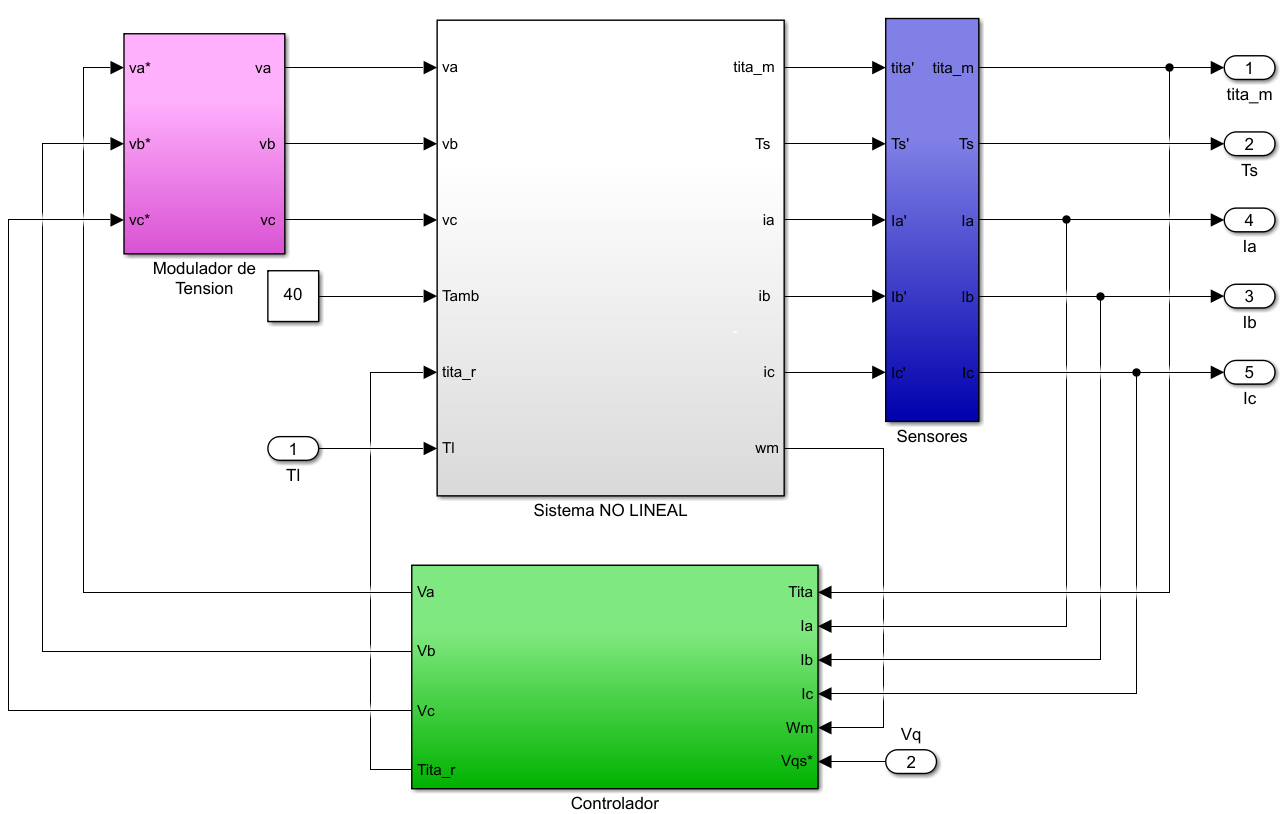
\includegraphics[width=1\textwidth]{realimentacion.png}
        \caption{Diagrama de bloques del sistema NL con restricción o ley de control mínima.}
    \end{figure}

    \begin{figure}[H]
        \centering
        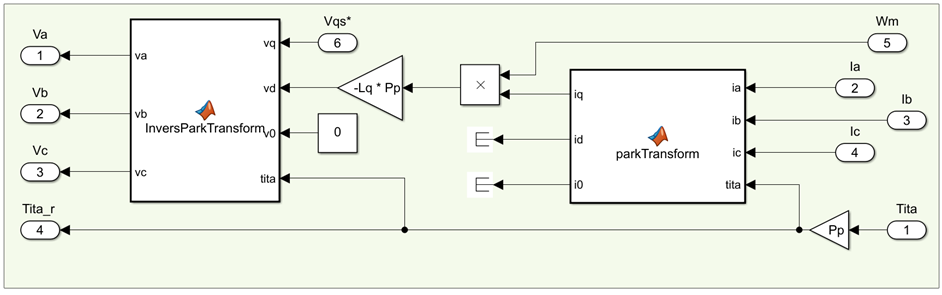
\includegraphics[width=1\textwidth]{controlador.png}
        \caption{Diagrama del controlador.}
    \end{figure}

    \item \textbf{Dinámica Residual}
    
    Al aplicar la ley de control mínimo supusimos que $i_{ds} = 0$, sin embargo, esto no es del todo cierto
    por lo que se debe tener en cuenta la dinámica residual de la corriente $i_{ds}$, la cual se puede
    modelar con la siguiente EDO:

    \begin{equation*}
        \begin{aligned}
        \frac{di_{ds}^r(t)}{dt} = \frac{1}{L_{d}}[-R_{s}(t)i_{ds}^r(t)] \\
        \frac{di_{ds}^r(t)}{dt} + \frac{R_{s}(t)}{L_{d}}i_{ds}^r(t) = 0 
        \end{aligned}
    \end{equation*} 

    La cual tiene como solución:

    \begin{equation}
        i_{ds}^r(t) = i_{ds}^r(0)e^{-\frac{R_{s}(t)}{L_{d}}t}
    \end{equation}

    Esta solución nos indica que el efecto de la dinámica residual es despreciable en el tiempo, ya que actúa como
    un sistema subamortiguado de primer orden.

    En régimen natural producirá un comportamiento no lineal sobre el sistema que esta dado por:

    \begin{equation}\label{eq.dinamica_residual}
        v_{qs}(t) = L_{q}\frac{di_{qs}^r(t)}{dt} + R_{s}i_{qs}^r(t) + P_{p}\omega_{m}(t)\lambda_{m}^{\prime r} + \mathbf{L_{d}i_{ds}^r(t)P_{p}\omega_{m}(t)}
    \end{equation}

    Incorporando la dinámica residual al modelo LTI:    

    \begin{equation}
        \begin{cases}
            \dot{\theta}_{m}(t) = \omega_{m}(t)\\
            \dot{\omega}_{m}(t) = -\frac{1}{J_{eq}}[\frac{3}{2}P_{p}\lambda_{m}^{\prime r} i_{qs}^r(t) - b_{eq}\omega_{m}(t)-\frac{T_{l}(t)}{r}]\\
            \dot{i}_{qs}^r(t) = \frac{1}{L_{q}}[v_{qs}^r(t) - R_{s}i_{qs}^r(t) - P_{p}\omega_{m}(t)\lambda_{m}^{\prime r}]\\
            \dot{i}_{ds}^r(t) = -\frac{R_{s}(t)}{L_{d}}i_{ds}^r(t) \\
            \dot{T}_{s}(t) = \frac{1}{C_[ts]}\{\frac{3}{2}R_{s}(t)[{i_{qs}^r}^2(t) + {i_{ds}^r}^2(t)] - \frac{1}{R_{ts-amb}}[T_{s}(t) - T_{amb}(t)]\}\\
        \end{cases}    
    \end{equation}

    \item \textbf{Restricción Ley de Control complementaria minima en el eje q}
    
    Para anular el efecto NL del acoplamiento de la dinámica residual podemos a partir de la
    \hyperref[eq.dinamica_residual]{ecuación (\ref*{eq.dinamica_residual})}
    plantear la siguiente restricción sobre el eje q de forma que la no linealidad se anule:

    \begin{equation}
        v_{qs}(t) = L_{q}\frac{di_{qs}^r(t)}{dt} + R_{s}i_{qs}^r(t) + P_{p}\omega_{m}(t)\lambda_{m}^{\prime r} + L_{d}i_{ds}^r(t)P_{p}\omega_{m}(t) - \mathbf{L_{d}i_{ds}^r(t)P_{p}\omega_{m}(t)}
    \end{equation}

    % IMAGEN DEL MODELO %

    A continuación se muestran los modelos LTI equivalente aumentado y el NL desacoplado con Ley de Control NL.

    \begin{figure}[H]
        \centering
        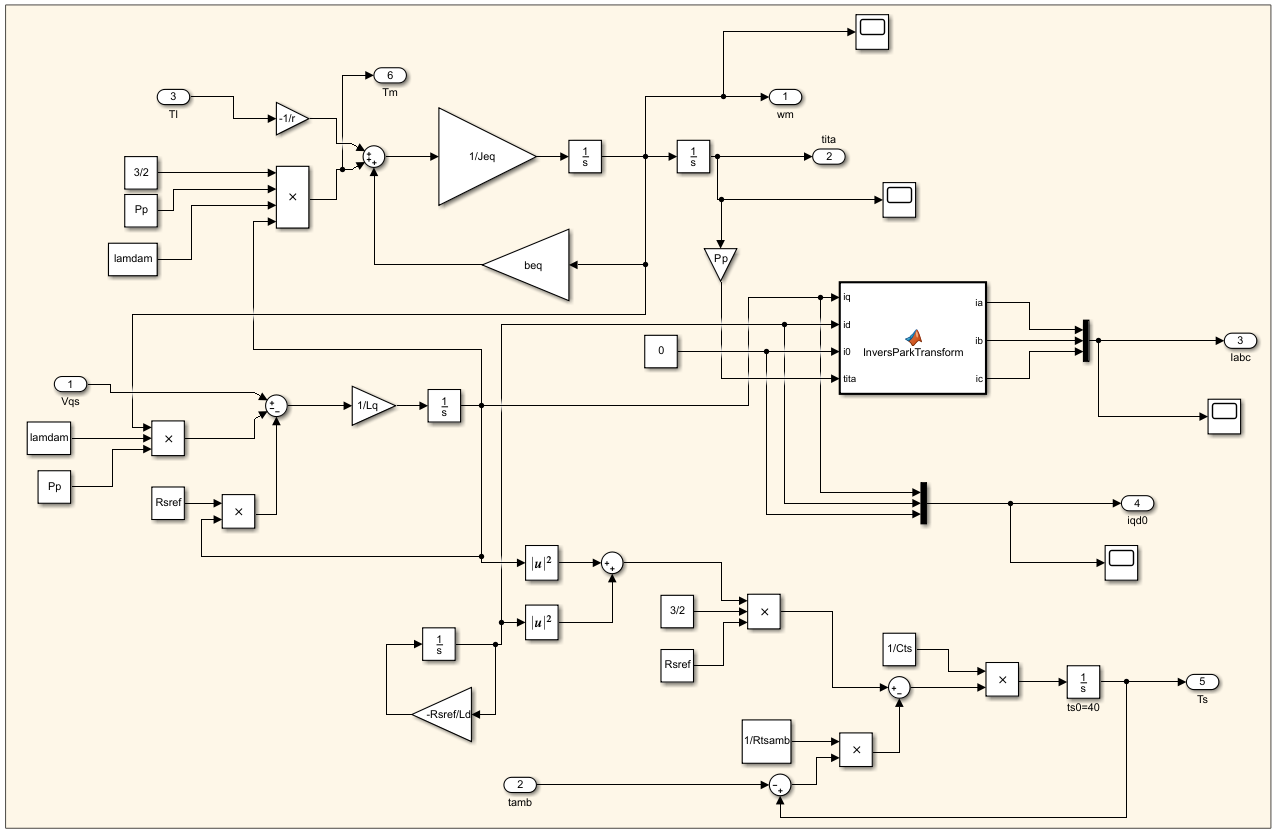
\includegraphics[width=1\textwidth]{LTI_aumentado1.png}
        \caption{Diagrama de bloques del modelo LTI equivalente aumentado.}
    \end{figure}

    \begin{figure}[H]
        \centering
        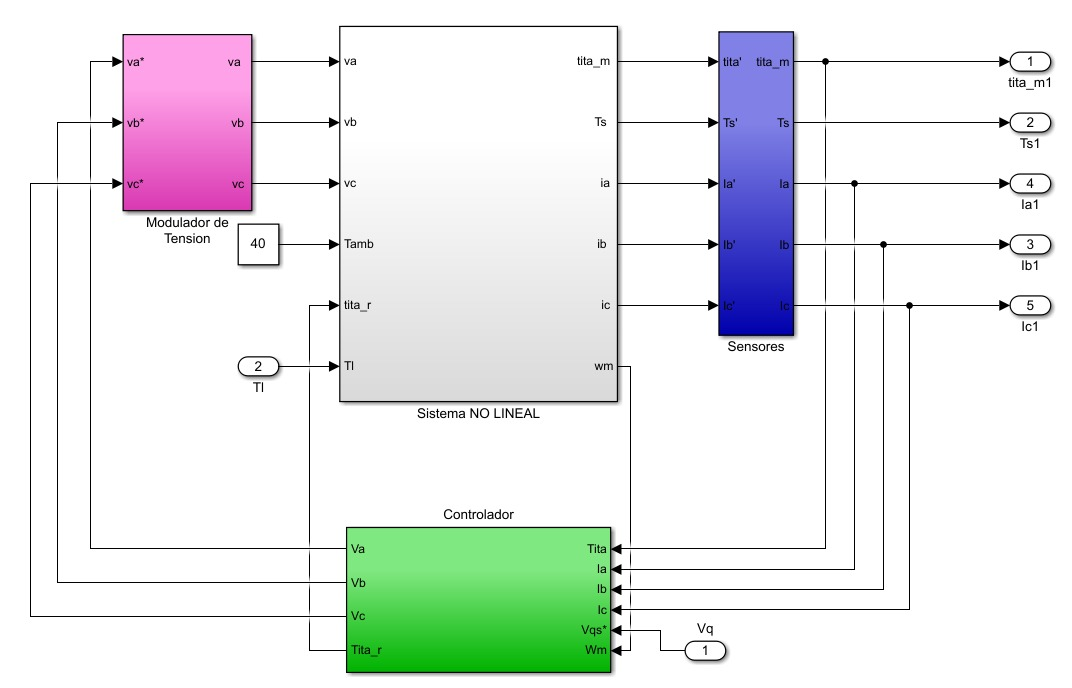
\includegraphics[width=1\textwidth]{LTI_AUMENTADO_Q.jpg}
        \caption{Diagrama de bloques del sistema NL con ley de control mínima en eje d y q.}
    \end{figure}

    \begin{figure}[H]
        \centering
        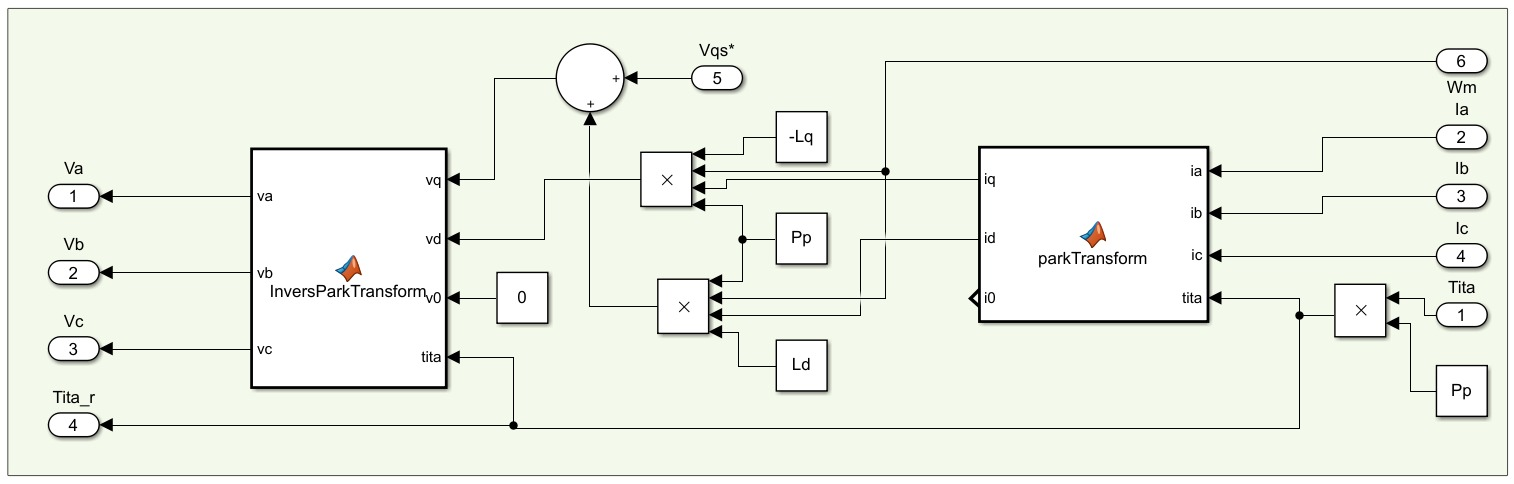
\includegraphics[width=1\textwidth]{LTI_AUMENTADO_Q_CONTROLADOR.jpg}
        \caption{Diagrama del controlador.}
    \end{figure}


\end{enumerate}

%-------------------- 5.1.2.d --------------------------%

\subsubsection{Comparación modelo dinámico LTI equivalente aumentado vs modelo dinámico global LPV}

El Modelo Dinámico Global LPV se basa en el concepto de Variabilidad de Parámetros Lineales (LPV), 
lo que significa que considera la variación de los parámetros en función de ciertas variables, como 
la corriente en directo $i^r_{ds}(t)$. Este enfoque tiene la ventaja de tener en cuenta la esencia no 
lineal del sistema, lo que permite una representación más precisa y realista del comportamiento del 
sistema en diferentes puntos de operación. Debido a esta consideración de parámetros variables, el 
modelo global LPV ofrece una mayor cantidad de puntos de trabajo en comparación con el modelo LTI 
equivalente.

Por otro lado, el Modelo Dinámico LTI Equivalente Aumentado es un caso particular del modelo LPV, 
donde se impone la restricción $i^r_{ds}(t) \equiv 0$, es decir, la corriente en directo se mantiene 
constante. Esta restricción conduce a un sistema lineal y más simple, lo que facilita el análisis 
matemático y el diseño de controladores. Sin embargo, esta simplicidad viene a expensas de la pérdida 
de la esencia no lineal del sistema real, lo que puede limitar la precisión de las predicciones en 
ciertos escenarios.

\begin{itemize}
    
    \item Respecto al par electromagnético:
    
    Recordando la
    \hyperref[eq.torque_electromagnetico]{ecuación (\ref*{eq.torque_electromagnetico})}
    que describe el comportamiento del Torque Electromagnético.
    Podemos observar que para motores de polos salientes $L_{d} > L_{q}$, entonces cuando $i_{ds}^r(t)$
    toma valores \textbf{positivos} el campo magnético se refuerza lo que aumenta el torque del
    motor. Si la corriente directa toma valores \textbf{negativos} el campo magnético se debilita 
    y disminuye el torque del motor. En el caso que $i_{ds}^r(t) = 0$, el flujo concatenado solamente esta afectado por 
    los imanes permanentes.

    \item Respecto al subsistema eléctrico:

    % Voltaje con minúsculas
    \begin{equation}
        \dot{i}_{ds}^r = \frac{1}{L_{d}}[v_{ds}(t) - R_{s}(t)i_{ds}^r(t) + L_{q}i_{qs}^r(t)P_{p}\omega_[m](t)] = 0
    \end{equation}
    \begin{equation}
        \omega_{m}(t) = \frac{-v_{ds}(t) + R_{s}(t)i_{ds}^r(t)}{L_{q}}
    \end{equation}

    En este caso, la velocidad del motor disminuye cuando la corriente $i_{ds}^r$ 
    aumenta. Por lo que podemos concluir que el torque reaccionara inversamente 
    a la velocidad.

\end{itemize}

En términos de diseño y control, los modelos lineales, como el LTI equivalente aumentado, son más 
fáciles de manejar matemáticamente y permiten el diseño de controladores óptimos con herramientas 
establecidas como el control óptimo y la teoría de control de retroalimentación. Además, son más 
eficientes computacionalmente, lo que facilita la simulación y el análisis rápido del sistema. Sin 
embargo, los modelos no lineales, como el LPV, ofrecen una mayor precisión y flexibilidad en la 
representación de sistemas reales complejos.

%-------------------- 5.1.2.e --------------------------%

\subsubsection{Funciones de transferencia para el modelo LTI}

Las funciones de transferencia nos permiten relacionar las salidas con las entradas del sistema.
Como nuestro sistema dispone de dos entradas obtendremos dos funciones de transferencia. Aplicando 
la transformada de Laplace $L[f(t)] = F(s)$ a las ecuaciones del modelo LTI (\ref{eq.lti}), ademas,
recordando que la transformada de Laplace posee la siguiente propiedad

\begin{equation}
        L[\dot{f}(t)] = s.F(s) - f(0)
\end{equation}

Entonces al aplicar la transformada y recordando que las condiciones iniciales son nulas, el 
modelo queda:

\begin{equation}
    \begin{cases}
        s.\Theta_{m}(s) = \Omega_{m}(s)\\
        s.\Omega_{m}(s) = \frac{1}{J_{eq}}.[\frac{3}{2}.P_{p}.\lambda_{m}^{\prime r}.I_{qs}^r(s) - b_{eq}.\Omega_m(s) - \frac{T_{l}(s)}{r}]\\
        s.I_{qs}^r(s) = \frac{1}{L_{q}}.[v_{qs}^r(s) - R_{s}.I_{qs}^r(s) - P_{p}.\Omega_{m}(s).\lambda_{m}^{\prime r}]\\
    \end{cases}
\end{equation}

Para obtener las funciones de transferencia del modelo, primero despejamos $I_{qs}^r(s)$
de la tercera ecuación y la reemplazamos en la segunda. Luego despejamos $\Omega_m(s)$ para 
finalmente reemplazarla en la primer ecuación y obtener la expresión que representa la salida del sistema: 

\begin{equation}
    \Theta_{m}(s) = \frac{\frac{3}{2}.P_{p}.\lambda_{m}^{\prime r}.v_{qs}(s) - \frac{1}{r}.(s.L_{q}+R_{s}).T_{l}(s)}{s^3.J_{eq}.L_{q} + s^2.(b_{eq}.L_{q} +  R_{s}.J_{eq}) + s.[b_{eq}.R_{s}+\frac{3}{2}.(P_{p}.\lambda_{m}^{\prime r})^2]}
\end{equation}

De esta expresión se obtienen las funciones de transferencia respecto de las entradas tension $v_{qs}(s)$ y torque $T_{l}(s)$

\begin{equation}\label{eq.trasnferencia_1}
    G_{1}(s) = \frac{\Theta_{m}(s)}{v_{qs}(s)} = \frac{\frac{3}{2}.P_{p}.\lambda_{m}^{\prime r}}{s^3.J_{eq}.L_{q} + s^2.(b_{eq}.L_{q} +  R_{s}.J_{eq}) + s.[b_{eq}.R_{s}+\frac{3}{2}.(P_{p}.\lambda_{m}^{\prime r})^2]}
\end{equation}

\begin{equation}\label{eq.transferencia_2}
    G_{2}(s) = \frac{\Theta_{m}(s)}{T_{l}(s)} = \frac{- \frac{1}{r}.(s.L_{q}+R_{s})}{s^3.J_{eq}.L_{q} + s^2.(b_{eq}.L_{q} +  R_{s}.J_{eq}) + s.[b_{eq}.R_{s}+\frac{3}{2}.(P_{p}.\lambda_{m}^{\prime r})^2]}
\end{equation}

%-------------------- 5.1.3 --------------------------%

\subsection{Análisis de Estabilidad}

Para realizar un análisis de estabilidad debemos primero determinar polos (ceros del denominador) del 
sistema a partir de la función de transferencia obtenida anteriormente:

\begin{equation}
    s^3.J_{eq}.L_{q} + s^2.(b_{eq}.L_{q} +  R_{s}.J_{eq}) + s.[b_{eq}.R_{s}+\frac{3}{2}.(P_{p}.\lambda_{m}^{\prime r})^2] = 0
\end{equation}

Utilizando Matlab para poder resolver este polinomio obtenemos que los valores que la satisfacen son:

\begin{align*}
    s_{1} &= 0\\
    s_{2} &= \frac{-(L_q.b_{eq} + R_s.J_{eq}) + sqrt{(L_q.b_{eq} + R_s.J_{eq})^2 - 4.J_{eq}.L_q.(R_s.b_eq + \frac{3}{2}.P_p^2.\lambda_{m}^{\prime r})^2}}{2.J_{eq}.L_q}\\
    s_{3} &= \frac{-(L_q.b_{eq} + R_s.J_{eq}) - sqrt{(L_q.b_{eq} + R_s.J_{eq})^2 - 4.J_{eq}.L_q.(R_s.b_eq + \frac{3}{2}.P_p^2.\lambda_{m}^{\prime r})^2}}{2.J_{eq}.L_q}
\end{align*}

Reemplazando los valores de los parámetros y teniendo en cuenta que $R_s$ puede variar con la temperatura entre 
$1,02\, \Omega$ y $1,32\, \Omega$ de manera lineal, se observa que los polos se encuentran en 
función de este valor dado que las demás valores son parámetros fijos del sistema.

Para determinar los ceros evaluamos  el numerador de la
\hyperref[eq.transferencia_2]{función de transferencia (\ref*{eq.transferencia_2})}
. De aquí notamos que solo $T_l(t)$ introduce ceros al sistema, obteniendo, al igual que en el caso 
de los polos, funciones dependientes de $Rs$.

\begin{equation*}
    s.L_q+ R_s = 0 \quad\quad\quad\to\quad\quad\quad s = - \frac{R_s}{L_q} = - \frac{R_s}{5,9.10^3}\\ 
\end{equation*}

Podemos hacer un gráfico en el plano imaginario sobre como varían estos valores según el valor de 
$R_s$. Asi obtenemos la siguiente figura:

\begin{figure}[H]
    \centering
    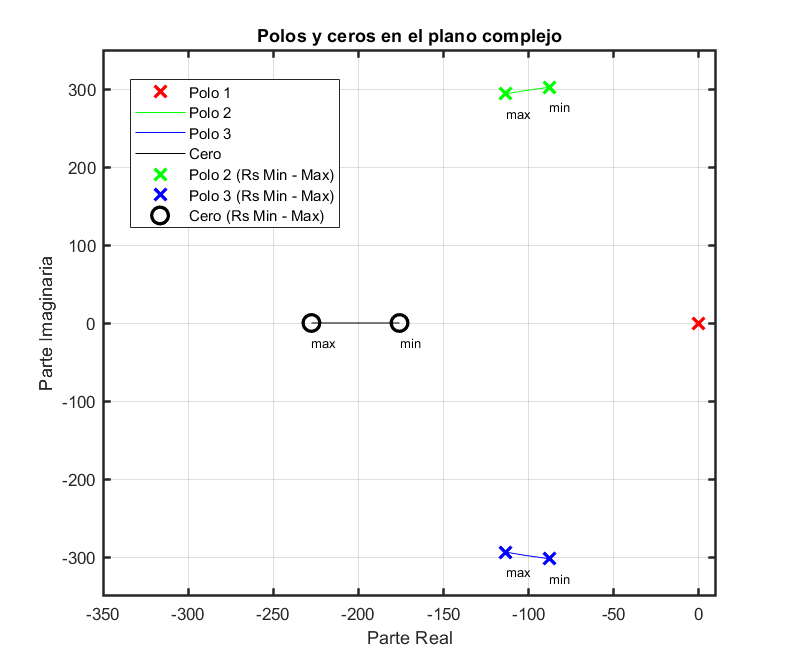
\includegraphics{polosyceros.png}
    \caption{Polos y ceros en función de $R_s$}
\end{figure}

En esta figura se grafican los sucesivos valores que pueden tomar los polos y el cero si variamos el 
valor de $R_s$. Notamos una pequeña disminución de la parte imaginaria con el aumento de esta variable, 
aunque esto es casi despreciable. También se logra visualizar la distancia al eje imaginario que 
tiene cada posible valor y sobre todo el valor mas cercano a esta (representa el caso menos 
amortiguado).

De la misma podemos concluir que a medida que el valor de la temperatura aumenta, aumentando $R_s$, el 
sistema se vuelve mas estable. Esto se puede ver ya que al aumentar la parte real negativa, los 
mismos vuelven la respuesta del sistema mas amortiguado.

Para obtener el valor de la frecuencia natural del sistema y el amortiguamiento relativo, podemos 
comparar la ecuación característica del sistema con la forma estándar que toma un sistema de tercer 
orden. Pero al trabajar sobre el polinomio característico, teniendo en cuenta que un polo es 0, 
podemos simplificar y compararlo con uno de orden 2:

\begin{equation}
    s^2 + 2.\xi.\omega_n.s + \omega_n^2 = 0
\end{equation}

Igualando ambas expresiones obtenemos los siguiente valores:

\begin{align*}
    \omega_n = \sqrt{\frac{R_s.b_{eq} + \frac{3}{2}.P_p^2.{\lambda_m^{\prime r}}^2}{J_{eq}.L_q}} \\
    \xi = \frac{L_q.b_{eq} + R_s.J_{eq}}{2.J_{eq}.L_q.\omega_n}
\end{align*}

Reemplazando los valores de los parámetros obtenemos que:

\begin{equation*}\begin{aligned}
    314,50\,rad/s < \omega_n < 314,72\,rad/s \\
    0.28 < \xi < 0.36 \quad\quad\quad\quad
\end{aligned}\end{equation*}

La frecuencia natural ($\omega_n$) no varia significativamente con $R_s$, en cambio el valor de $\xi$
se ve influenciado de mayor manera aunque siempre se mantiene en rangos menores a 1, lo que 
indica que es un sistema subamortiguado.

Podemos ver como varían estos valores en los siguientes gráficos:

\begin{figure}[H]
    \centering
    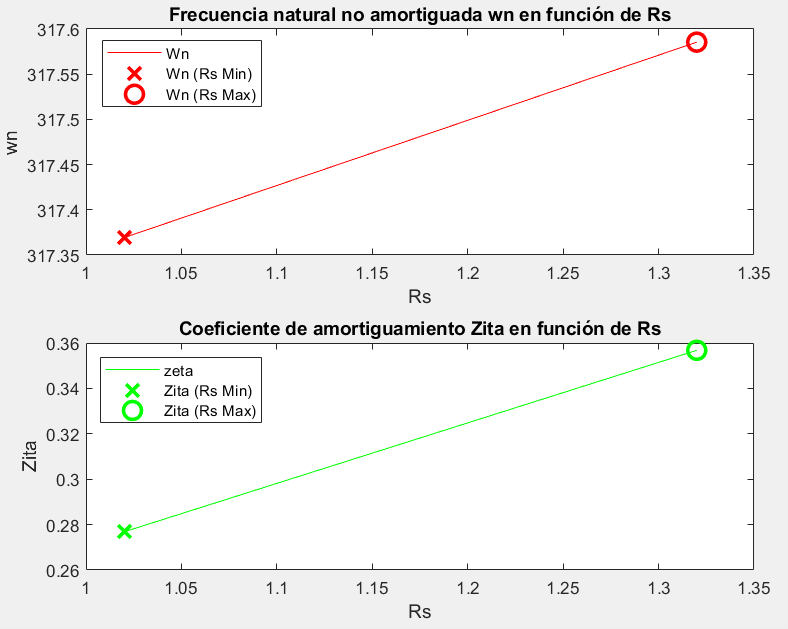
\includegraphics{frecuancia_amortiguamiento_rs.png}
    \caption{Frecuencia natural y amortiguamiento en función de $R_s$}
\end{figure}

%-------------------- 5.1.4 --------------------------%

\subsection{Análisis de Observabilidad}

Para realizar el análisis de observabilidad completa de estados para el modelo LTI equivalente 
aumentado desde la salida $\theta_m$, evaluamos el rango de la matriz de observabilidad "$O$".

En este caso la matriz de observabilidad, teniendo en cuenta que es un sistema de 3er orden, 
debe tener orden 3 también. Asi:

\begin{equation}
    O = \begin{bmatrix}
        C \\
        C.A \\
        C.A^2
    \end{bmatrix}
\end{equation}

Con:

\begin{equation}
    C = \begin{bmatrix}
        1 & 0 & 0
    \end{bmatrix}
\end{equation}

\begin{equation}
    C.A = 
    \begin{bmatrix}
        1 & 0 & 0
    \end{bmatrix}.
    \begin{bmatrix}
        0 & 1 & 0 \\
        0 & -\frac{b_{eq}}{J_{eq}} & \frac{3.P_p.\lambda_m^{\prime r}}{2.J_{eq}} \\
        0 & -\frac{P_p.\lambda_m^{\prime r}}{L_q} & -\frac{R_s}{L_q}
    \end{bmatrix}
    =
    \begin{bmatrix}
        0 & 1 & 0
    \end{bmatrix}
\end{equation}

\begin{equation}
    C.A^2 =
    \begin{bmatrix}
        1 & 0 & 0
    \end{bmatrix}.
    \begin{bmatrix}
        0 & 1 & 0 \\
        0 & -\frac{b_{eq}}{J_{eq}} & \frac{3.P_p.\lambda_m^{\prime r}}{2.J_{eq}} \\
        0 & -\frac{P_p.\lambda_m^{\prime r}}{L_q} & -\frac{R_s}{L_q}
    \end{bmatrix}.
    \begin{bmatrix}
        0 & 1 & 0 \\
        0 & -\frac{b_{eq}}{J_{eq}} & \frac{3.P_p.\lambda_m^{\prime r}}{2.J_{eq}} \\
        0 & -\frac{P_p.\lambda_m^{\prime r}}{L_q} & -\frac{R_s}{L_q}
    \end{bmatrix}
    =
    \begin{bmatrix}
        0 & -\frac{b_{eq}}{J_{eq}} & \frac{3.P_p.\lambda_m^{\prime r}}{2.J_{eq}}
    \end{bmatrix}
\end{equation}

Por lo tanto:

\begin{equation}
    O = 
    \begin{bmatrix}
        1 & 0 & 0 \\
        0 & 1 & 0 \\
        0 & -\frac{b_{eq}}{J_{eq}} & \frac{3.P_p.\lambda_m^{\prime r}}{2.J_{eq}}
    \end{bmatrix}
\end{equation}

El rango de esta matriz es 3, por lo tanto el sistema es completamente observable a partir de la 
salida $\theta_m$.

Estrictamente debemos decir que el sistema es parcialmente observable a partir de tener la posición 
como variable de salida ya que no se pueden obtener los estados de $i_ds^r$ ni $T_s^°$.

Podemos realizar el mismo análisis a partir de tener como variable medida la velocidad, utilizando 
un taco generador. En este caso tendremos:

\begin{equation}
    C = \begin{bmatrix}
        0 & 1 & 0
    \end{bmatrix}
\end{equation}

\begin{equation*}
    C.A = 
    \begin{bmatrix}
        0 & 1 & 0
    \end{bmatrix}.
    \begin{bmatrix}
        0 & 1 & 0 \\
        0 & -\frac{b_{eq}}{J_{eq}} & \frac{3.P_p.\lambda_m^{\prime r}}{2.J_{eq}} \\
        0 & -\frac{P_p.\lambda_m^{\prime r}}{L_q} & -\frac{R_s}{L_q}
    \end{bmatrix}
    =
    \begin{bmatrix}
        0 & -\frac{b_{eq}}{J_{eq}} & \frac{3.P_p.\lambda_m^{\prime r}}{2.J_{eq}}
    \end{bmatrix}
\end{equation*}

\begin{equation*}
    C.A^2 =
    \begin{bmatrix}
        0 & 1 & 0
    \end{bmatrix}.
    \begin{bmatrix}
        0 & 1 & 0 \\
        0 & -\frac{b_{eq}}{J_{eq}} & \frac{3.P_p.\lambda_m^{\prime r}}{2.J_{eq}} \\
        0 & -\frac{P_p.\lambda_m^{\prime r}}{L_q} & -\frac{R_s}{L_q}
    \end{bmatrix}.
    \begin{bmatrix}
        0 & 1 & 0 \\
        0 & -\frac{b_{eq}}{J_{eq}} & \frac{3.P_p.\lambda_m^{\prime r}}{2.J_{eq}} \\
        0 & -\frac{P_p.\lambda_m^{\prime r}}{L_q} & -\frac{R_s}{L_q}
    \end{bmatrix}
    =
    \begin{bmatrix}
        0 & -\frac{b_{eq}}{J_{eq}} - \frac{3.P_p^2.{\lambda_m^{\prime r}}^2}{2.J_{eq}.L_q} & \frac{3.b_{eq}.P_p.\lambda_m^{\prime r}}{2.J_{eq}^2}
    \end{bmatrix}
\end{equation*}

Entonces: 

\begin{equation*}
    O = 
    \begin{bmatrix}
        0 & 1 & 0 \\
        0 & -\frac{b_{eq}}{J_{eq}} & \frac{3.P_p.\lambda_m^{\prime r}}{2.J_{eq}} \\
        0 & -\frac{b_{eq}}{J_{eq}} - \frac{3.P_p^2.{\lambda_m^{\prime r}}^2}{2.J_{eq}.L_q} & \frac{3.b_{eq}.P_p.\lambda_m^{\prime r}}{2.J_{eq}^2}
    \end{bmatrix}
\end{equation*}

El rango de esta matriz es 2, por lo tanto podemos afirmar que el sistema no es observable a 
partir de la salida $\omega_n$. Esto se debe a que, conociendo la velocidad, no se puede estimar la 
posición sin conocer la condición inicial de la misma.

%-------------------- 5.1.5 --------------------------%

\subsection{Análisis de Controlabilidad}

Para afirmar si el sistema es controlable a partir de la entrada manipulada estipulada 
$v_{qs}^r(t)$ debemos estudiar el rango de la matriz de controlabilidad $C$. Esta nos 
proporcionara la certeza de si el sistema LTI se puede transferir desde cualquier estado inicial
a cualquier otro estado, mediante un vector de control no restringido en un intervalo de tiempo 
finito.

Para este caso la matriz de Controlabilidad es:

\begin{equation}
    C = 
    \begin{bmatrix}
        B & A.B & A^2.B
    \end{bmatrix}
\end{equation}

Con:

\begin{equation*}
    B = 
    \begin{bmatrix}
        0 \\
        0 \\
        \frac{1}{L_q}
    \end{bmatrix}
\end{equation*}

\begin{equation*}
    A.B = 
    \begin{bmatrix}
        0 & 1 & 0 \\
        0 & -\frac{b_{eq}}{J_{eq}} & \frac{3.P_p.\lambda_m^{\prime r}}{2.J_{eq}} \\
        0 & -\frac{P_p.\lambda_m^{\prime r}}{L_q} & -\frac{R_s}{L_q}
    \end{bmatrix}.
    \begin{bmatrix}
        0 \\
        0 \\
        \frac{1}{L_q}
    \end{bmatrix}
    =
    \begin{bmatrix}
        0 \\
        \frac{3.P_p.\lambda_m^{\prime r}}{2.J_{eq}} \\
        -\frac{R_s}{L_q}
    \end{bmatrix}
\end{equation*}

\begin{equation*}
    A^2.B =
    \begin{bmatrix}
        0 & 1 & 0 \\
        0 & -\frac{b_{eq}}{J_{eq}} & \frac{3.P_p.\lambda_m^{\prime r}}{2.J_{eq}} \\
        0 & -\frac{P_p.\lambda_m^{\prime r}}{L_q} & -\frac{R_s}{L_q}
    \end{bmatrix}.
    \begin{bmatrix}
        0 & 1 & 0 \\
        0 & -\frac{b_{eq}}{J_{eq}} & \frac{3.P_p.\lambda_m^{\prime r}}{2.J_{eq}} \\
        0 & -\frac{P_p.\lambda_m^{\prime r}}{L_q} & -\frac{R_s}{L_q}
    \end{bmatrix}.
    \begin{bmatrix}
        0 \\
        0 \\
        \frac{1}{L_q}
    \end{bmatrix}
    =
    \begin{matrix}
        \frac{3.P_p.\lambda_m^{\prime r}}{2.J_{eq}.L_q} \\
        -\frac{3.P_p.b_{eq}.\lambda_m^{\prime r}}{2.J_{eq}^2.L_q} - \frac{3.P_p.\lambda_m^{\prime r}.R_s}{2.J_{eq}.L_q^2} \\
        \frac{3.P_p.\lambda_m^{\prime r}}{2.J_{eq}^2}
    \end{matrix}
\end{equation*}

Entonces:

\begin{equation*}
    C = 
    \begin{bmatrix}
        0 & 0 & \frac{3.P_p.\lambda_m^{\prime r}}{2.J_{eq}.L_q} \\
        0 & \frac{3.P_p.\lambda_m^{\prime r}}{2.J_{eq}} & -\frac{3.P_p.b_{eq}.\lambda_m^{\prime r}}{2.J_{eq}^2.L_q} - \frac{3.P_p.\lambda_m^{\prime r}.R_s}{2.J_{eq}.L_q^2} \\
        \frac{1}{L_q} & -\frac{3.P_p.b_{eq}.\lambda_m^{\prime r}}{2.J_{eq}^2.L_q} - \frac{3.P_p.\lambda_m^{\prime r}.R_s}{2.J_{eq}.L_q^2} & \frac{3.P_p.\lambda_m^{\prime r}}{2.J_{eq}^2}
    \end{bmatrix}
\end{equation*}

En este caso el rango de la matriz de controlabilidad es 3, por lo tanto podemos afirmar que el 
sistema LTI equivalente simplificado es controlable desde la entrada indicada. Cabe aclarar que 
a partir de $v_{qs}^r(t)$ no es posible controlar la salida de los estados $i_ds^r$ ni $T_s^°$ 
del sistema LTI equivalente aumentado. Estas podrían controlares si se agrega entradas de control 
destinadas específicamente para esto.

%-------------------- 5.1.6 --------------------------%

\subsection{Simulación Dinámica}

Realizamos uan simulación dinámica en el dominio del tiempo, comparando el modelo NL completo 
desacoplado con Ley de control NL con el modelo LTI equivalente aumentado.

\subsubsection{Respuesta del estado interno a pulso de consigna de tension de estador en el eje $q$}

La consiga es la que se muestra en la siguiente figura:

\begin{figure}[H]
    \centering
    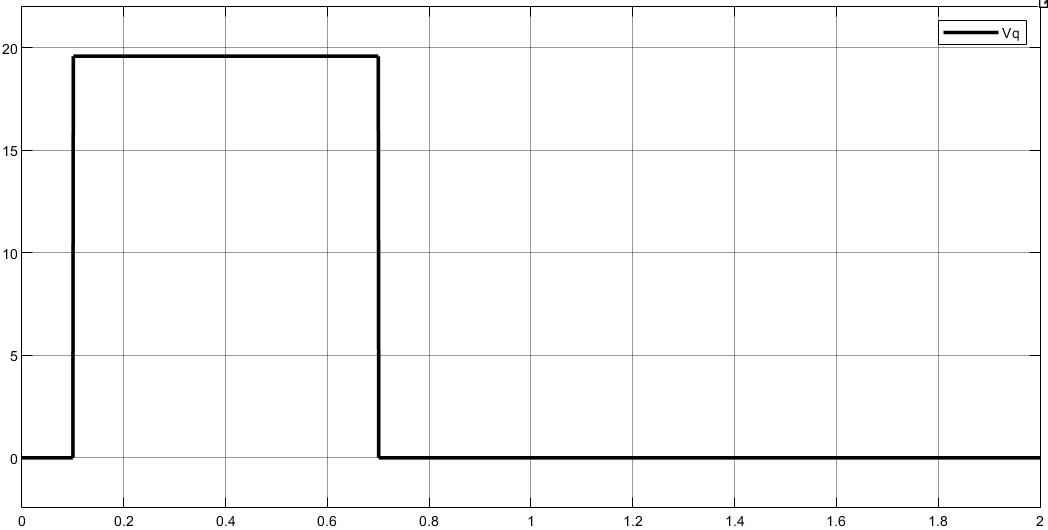
\includegraphics[width=0.85\textwidth]{5.1.6_consigna.jpg}
    \caption{Consigna $v_q(t)$.}
\end{figure}

Como se puede observar toma el valor de $+19.596 \, V$ en el intervalo de tiempo de $0.1 \, s$ a $0.7 \, s$.
Esta consigna se superpone con un doble pulso de torque de carga como el que se muestra en la figura (\ref{fig:torque_carga}).
$T_l(t)$ toma su  valor máximo ($+6.28 \, N.m$) de $0.3 \, s$ a $0.5 \, s$ y su mínimo ($-6.28 \, N.m$) de $0.5 \, s$ a $0.9 \, s$.

\begin{figure}[H]
    \centering
    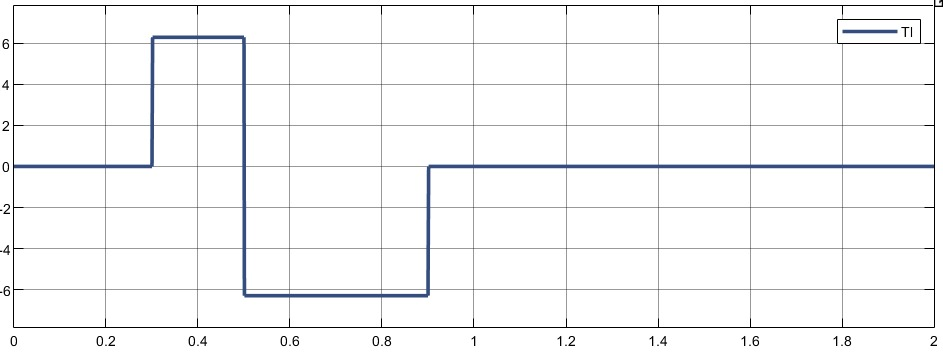
\includegraphics[width=0.85\textwidth]{5.1.6_carga2.jpg}
    \caption{Carga $T_l(t)$}
    \label{fig:torque_carga}
\end{figure}

A continuación se mostraran las respuestas del sistema a la consigna de tensión de estator en el eje $q$.
Se ira comparando cada variable una a una entre el LTI equivalente aumentado y el modelo NL con Ley de control NL, 
en ese mismo orden.

\begin{figure}[H]
    \centering
    \begin{subfigure}[b]{0.8\textwidth}
        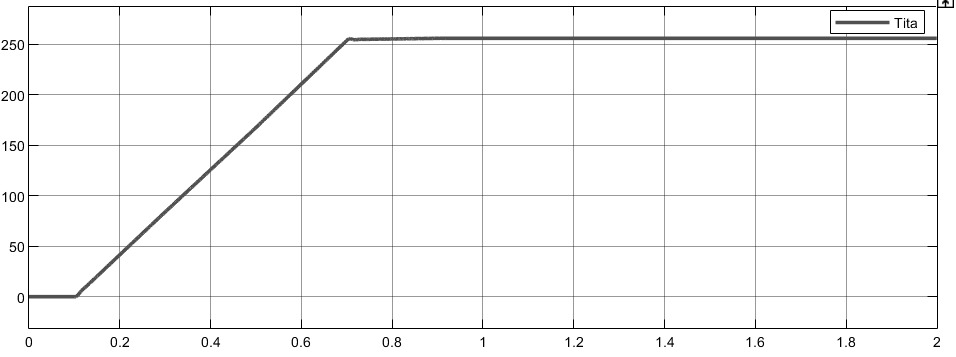
\includegraphics[width=\textwidth]{5.1.6_tita.jpg}
    \end{subfigure}
    \begin{subfigure}[b]{0.8\textwidth}
        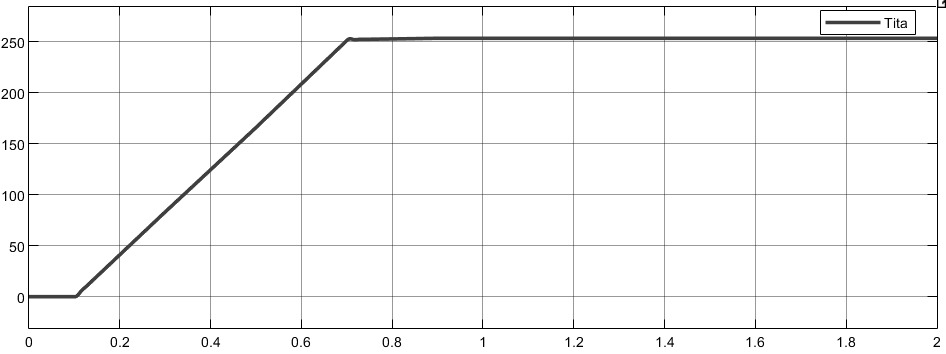
\includegraphics[width=1\textwidth]{5.1.6_tita_NL.jpg}
    \end{subfigure}
    \caption{Respuesta de la posición ($\theta_m(t)$) en función del tiempo.}
    \label{fig:posicion}
\end{figure}

\begin{figure}[H]
    \centering
    \begin{subfigure}[b]{0.8\textwidth}
        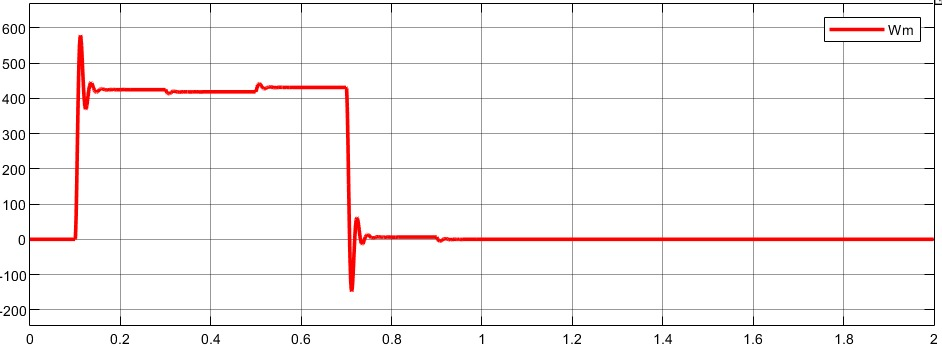
\includegraphics[width=\textwidth]{5.1.6_omega.jpg}
    \end{subfigure}
    \begin{subfigure}[b]{0.8\textwidth}
        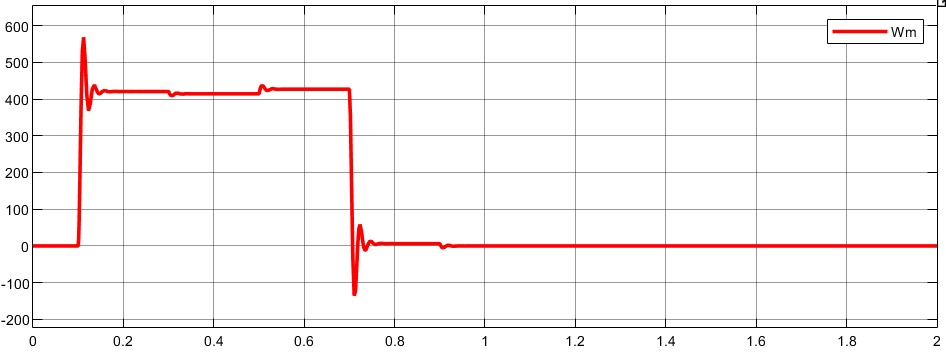
\includegraphics[width=1\textwidth]{5.1.6_omega_NL.jpg}
    \end{subfigure}
    \caption{Respuesta de la velocidad ($\omega_m(t)$) en función del tiempo.}
    \label{fig:velocidad}
\end{figure}

\begin{figure}[H]
    \centering
    \begin{subfigure}[b]{0.8\textwidth}
        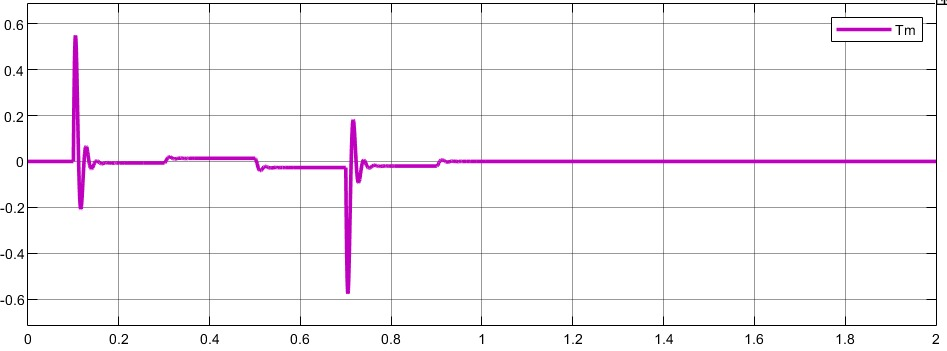
\includegraphics[width=\textwidth]{5.1.6_torque.jpg}
    \end{subfigure}
    \begin{subfigure}[b]{0.8\textwidth}
        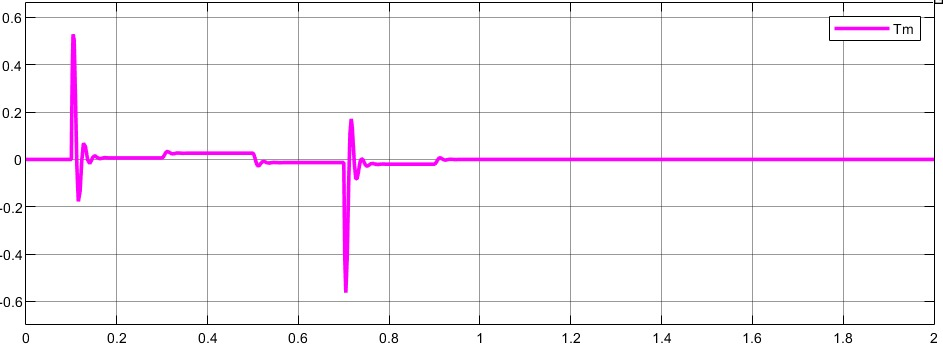
\includegraphics[width=1\textwidth]{5.1.6_torque_NL.jpg}
    \end{subfigure}
    \caption{Respuesta del torque ($T_m(t)$) en función del tiempo.}
    \label{fig:torque_electromagentico}
\end{figure}

\begin{figure}[H]
    \centering
    \begin{subfigure}[b]{0.8\textwidth}
        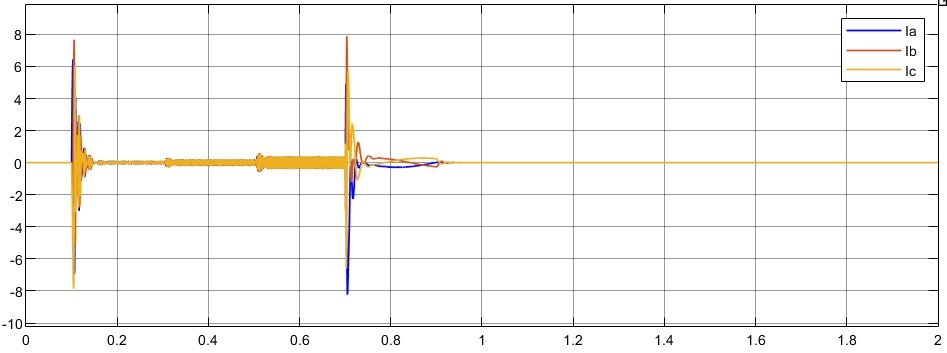
\includegraphics[width=\textwidth]{5.1.6_iabc.jpg}
    \end{subfigure}
    \begin{subfigure}[b]{0.8\textwidth}
        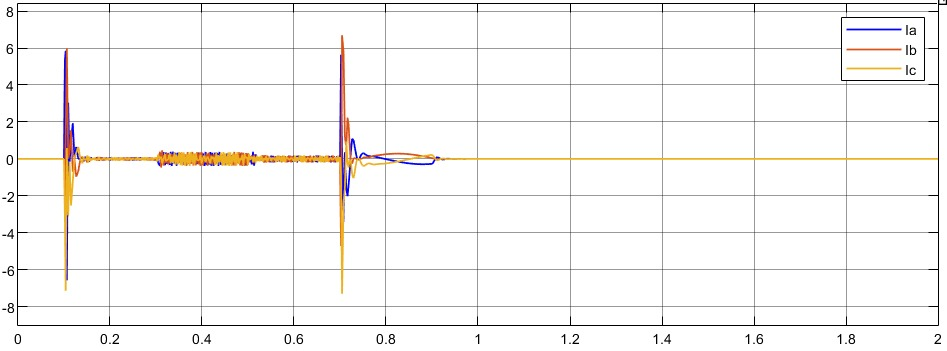
\includegraphics[width=1\textwidth]{5.1.6_iabc_NL.jpg}
    \end{subfigure}
    \caption{Respuesta de las corrientes ($i_{abc}(t)$) en función del tiempo.}
    \label{fig:iabc}
\end{figure}

\begin{figure}[H]
    \centering
    \begin{subfigure}[b]{0.8\textwidth}
        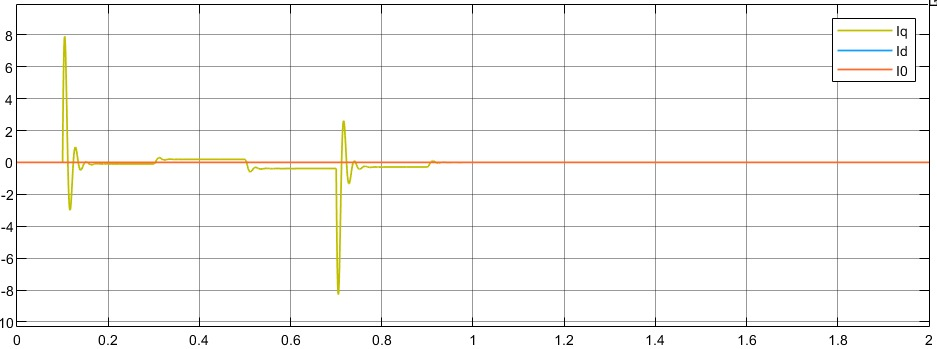
\includegraphics[width=\textwidth]{5.1.6_iqd0.jpg}
    \end{subfigure}
    \begin{subfigure}[b]{0.8\textwidth}
        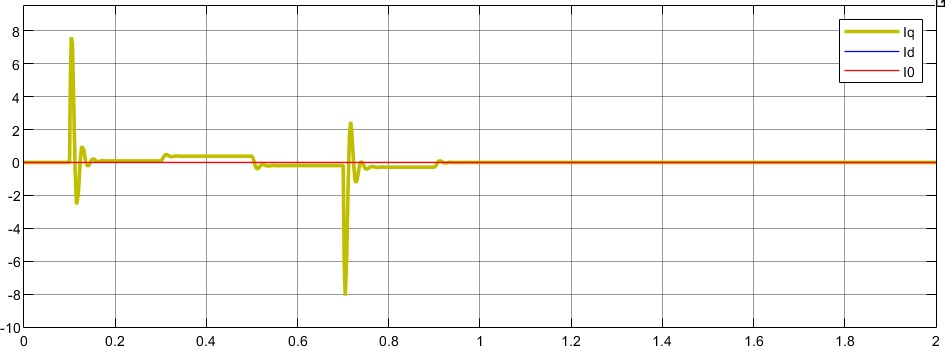
\includegraphics[width=1\textwidth]{5.1.6_iqd0_NL.jpg}
    \end{subfigure}
    \caption{Respuesta de las corrientes ($i_{qd0}(t)$) en función del tiempo.}
    \label{fig:iqd0}
\end{figure}

\begin{figure}[H]
    \centering
    \begin{subfigure}[b]{0.8\textwidth}
        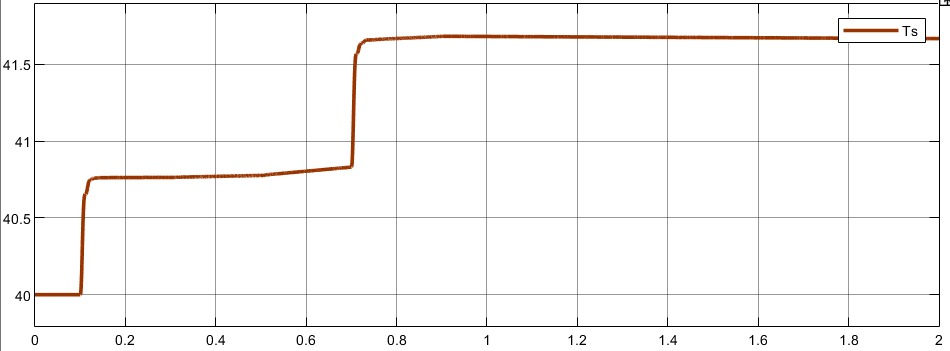
\includegraphics[width=\textwidth]{5.1.6_temperatura.jpg}
    \end{subfigure}
    \begin{subfigure}[b]{0.8\textwidth}
        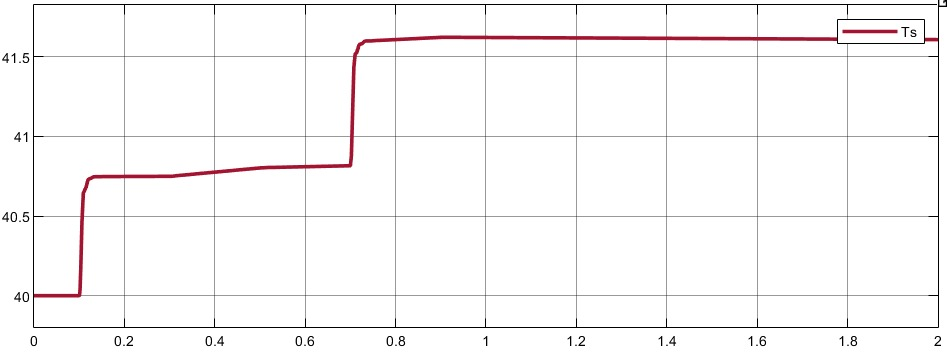
\includegraphics[width=1\textwidth]{5.1.6_temperatura_NL.jpg}
    \end{subfigure}
    \caption{Respuesta de la temperatura ($T_s(t)$) en función del tiempo.}
    \label{fig:temperatura}
\end{figure}

\begin{figure}[H]
    \centering
    \begin{subfigure}[b]{0.8\textwidth}
        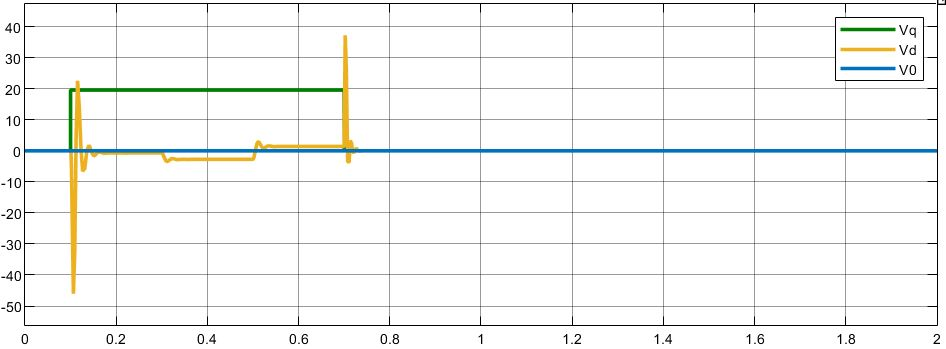
\includegraphics[width=\textwidth]{5.1.6_vqd0.jpg}
    \end{subfigure}
    \begin{subfigure}[b]{0.8\textwidth}
        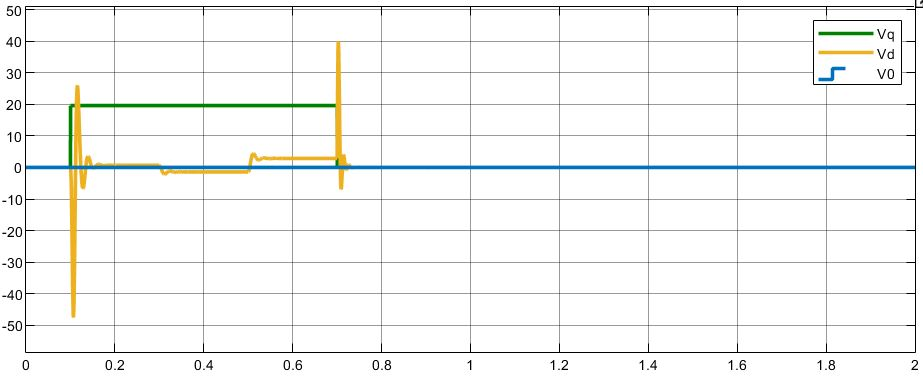
\includegraphics[width=1\textwidth]{5.1.6_vqd0_NL.jpg}
    \end{subfigure}
    \caption{Respuesta de la tensión ($v_{qd0}(t)$) en función del tiempo.}
    \label{fig:temperatura}
\end{figure}

\begin{figure}[H]
    \centering
    \begin{subfigure}[b]{0.8\textwidth}
        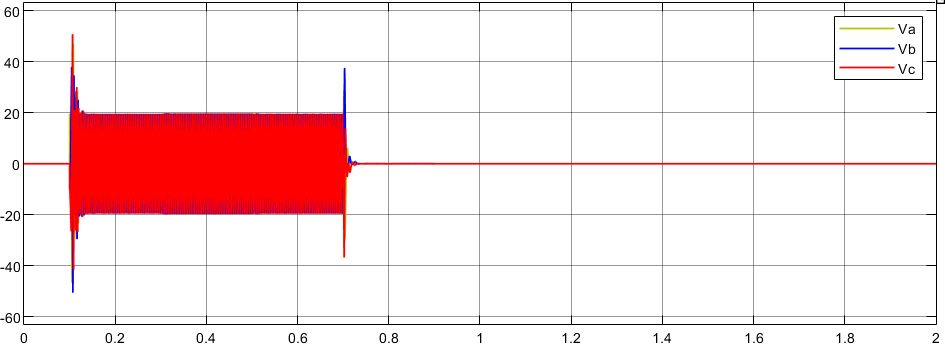
\includegraphics[width=\textwidth]{5.1.6_vabc.jpg}
    \end{subfigure}
    \begin{subfigure}[b]{0.8\textwidth}
        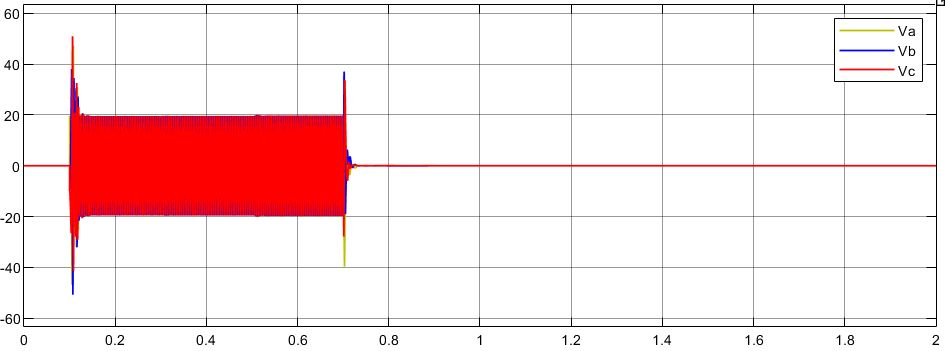
\includegraphics[width=1\textwidth]{5.1.6_vabc_NL.jpg}
    \end{subfigure}
    \caption{Respuesta de la tensión ($v_{abc}(t)$) en función del tiempo.}
    \label{fig:temperatura}
\end{figure}

De la Figura (\ref{fig:posicion}) se puede observar que la posición del rotor ($\theta_m(t)$)
varia casi linealmente en el periodo en el que la consiga de tensión en el eje $q$ es positiva.

La velocidad ($\omega_m(t)$) en la Figura (\ref{fig:velocidad}) pasa por un transitorio luego 
se estabiliza a un valor constante. En $0.3 \, s$, que es cuando comienza el doble pulso del 
torque de carga, se observa una leve decaimiento de la velocidad a la vez que el torque electromagnético
de la Figura (\ref{fig:torque_electromagentico}) aumenta para compensar el torque de carga.
De forma opuesta, cuando tenemos un torque de carga negativo ($t = 0.5 \, s$), el torque electromagnético 
disminuye y la velocidad angular aumenta.

Las figura de las corrientes (\ref{fig:iabc}) y (\ref{fig:iqd0}) muestra que en los transitorios del torque electromagnético
se producen picos de corriente. Esto se debe a que el torque electromagnético es proporcional a la corriente.
Estos picos produce que en la Figura de la temperatura (\ref{fig:temperatura}) se produzcan aumentos de esta.
La temperatura tiene un comportamiento escalonado debido a los dos transitorios que se producen.
Es posible observar también que al momento de activarse el torque de carga, la temperatura tiene una 
pendiente mayor, esto se debe a que el torque electromagnético aumento para compensar el de carga.

Para ambos modelos encontramos un comportamiento bastante similar, lo cual nos indica que el modelo LTI
es una buena aproximación del modelo NL. Esto se debe a que como ya se ha mencionado anteriormente, la 
variación de la temperatura es muy pequeña, por lo que no influye significativamente en los valores de $R_s$.

Podemos observar en la siguiente figura que la Ley de control aplicada es efectiva, ya que la corriente
en ele eje $d$ toma un rango de valores muy pequeños.

\begin{figure}[H]
    \centering
    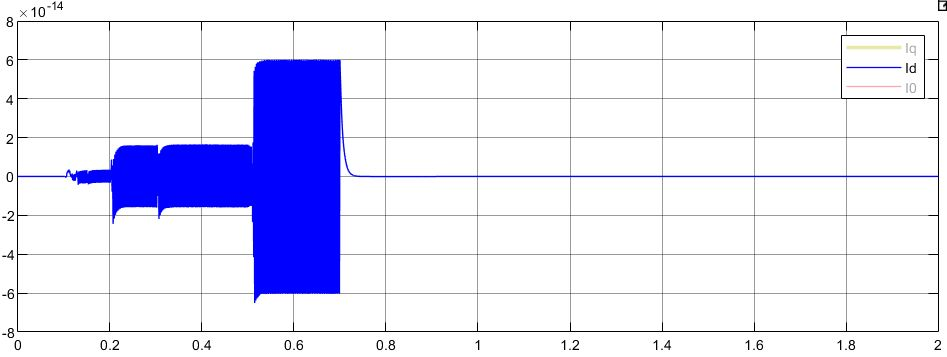
\includegraphics[width=0.8\textwidth]{5.1.6_id.jpg}
    \caption{Respuesta de la corriente en el eje $d$ ($i_d(t)$) en función del tiempo.}
\end{figure}

Estas perturbaciones se deben a los transitorios ya mencionados del torque, aunque también se observa 
el decaimiento que esta tiene que cumple con el comportamiento predicho en la dinámica residual. 

Finalmente mostramos los cuadrantes de operación de la maquina eléctrica.

\begin{figure}[H]
    \centering
    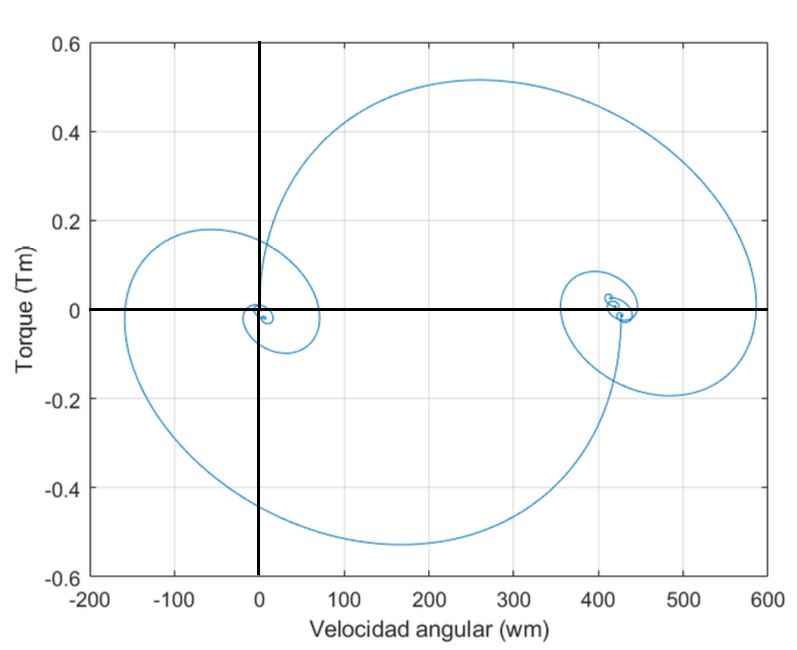
\includegraphics[width=0.8\textwidth]{5.1.6_torque_velocidad.png}
    \caption{Cuadrantes de operación de la maquina eléctrica.}
\end{figure}

De esta figura podemos observar que la maquina trabaja en los 4 cuadrantes, esto quiere decir que trabaja como 
motor y como generador. Ademas se puede determinar dos puntos de equilibrio, uno correspondiente al punto 
de trabajo de la maquina, cuando esta en motorización. El otro corresponde a la posición de la de apagado.
Las oscilaciones que se presentan al rededor de estos puntos son debido a los cambios del torque de carga.

\subsubsection{Velocidad y corriente final de establecimiento luego de cada transitorio}

Determinaremos de forma gráfica, utilizando el modelo NL completo desacoplado con ley de control  NL, 
distintas características que son de vital importancia para analizar el comportamiento de la velocidad 
y corriente.

Los distintos valores de tiempo utilizados son: T1 = 0.1 s, T2=0.3 s, T3 = 0.5 s, T4 = 0.7 s y T5=0.9 s. 
Estos equivalen a los tiempos en el que la consigna o el torque de carga cambian de valor.

\begin{table}[H]
    \centering
    \begin{tabular}{|c|c|c|c|c|c|}
        \hline
        & \multicolumn{5}{c|}{Velocidad Angular} \\
        \hline
        Tiempo & T1 & T2 & T3 & T4 & T5 \\
        \hline
        Valor Final [rad/s] & 420 & 414 & 427 & 6.33 & 0 \\
        \hline
        Tiempo de Crecimiento [ms] & 4.50 & 2.18 & 2.35 & 4.68 & 2.56 \\
        \hline
        Tiempo de Establecimiento [ms] & 126 & 356 & 555 & 749 & 972 \\
        \hline
        Sobre pico [rad/s] & 144 & 5.23 & 10.71 & 146 & 5.31 \\
        \hline
    \end{tabular}
    \caption{Características de la velocidad angular.}
\end{table}

\begin{table}[H]
    \centering
    \begin{tabular}{|c|c|c|c|c|c|}
        \hline
        & \multicolumn{5}{c|}{Corriente} \\
        \hline
        Tiempo & T1 & T2 & T3 & T4 & T5 \\
        \hline
        Valor Final [A]& 0.09 & 0.38 & -0.19 & -0.28 & 0 \\
        \hline
        Tiempo de Crecimiento [ms] & 0.02 & 3.40 & 3.41 & 0.01 & 3.23 \\
        \hline
        Tiempo de Establecimiento [ms] & 161 & 345 & 568 & 763 & 972 \\
        \hline
        Sobre pico [A] & 7.82 & 0.09 & 0.18 & 7.77 & 0.09 \\
        \hline
    \end{tabular}
    \caption{Características de la corriente.}
\end{table}

Los resultados obtenidos en el sistema LTI son muy parecidos y se determino no introducirlos. ya 
que el método gráfico es muy sensible y se pueden ver variaciones entre los dos modelos que no 
son concisos. Por otro lado es importante remarcar que dichas características son muy parecidos 
si comparamos valor por valor. Esto es debido a la poca variación que se tiene al trabajar de una 
forma u la otra. 

En el estudio de las acciones externas sobre el sistema, se nota que tanto la velocidad angular como 
el torque electromagnético responden de manera diferente a ciertos cambios. La velocidad angular
muestra una mayor sensibilidad ante variaciones de tensión, mientras que el torque electromagnético 
se ve más influenciado por cambios en el torque de perturbación.

A pesar de las diferencias en sus respuestas transitorias, al analizar las funciones que relacionan 
estas magnitudes con sus respectivas entradas, se observa que comparten similitudes. Estas similitudes 
se explican por las ganancias que afectan a las entradas correspondientes en cada expresión. 
Específicamente, la corriente/torque motor presenta una mayor ganancia respecto a la entrada perturbada 
en comparación con la velocidad angular. Por otro lado, la corriente/torque motor muestra una menor 
ganancia con respecto a la tensión en comparación con la velocidad angular.

\subsubsection{Comparación de distintas condiciones iniciales}

Las siguientes imágenes muestran el comportamiento de la corriente en tiempo real al seleccionar dos 
estados iniciales diferentes, $i^r_{ds}(0) = 0.5 \, A$ e $i^r_{ds}(0) = -0.5 \, A$, en dos modelos.

Primero mostramos los resultados obtenidos en el modelo "Global NL con ley de control NL".

\begin{itemize}
    \item $i^r_{ds}(0) = 0.5 A$
    
    \begin{figure}[H]
        \centering
        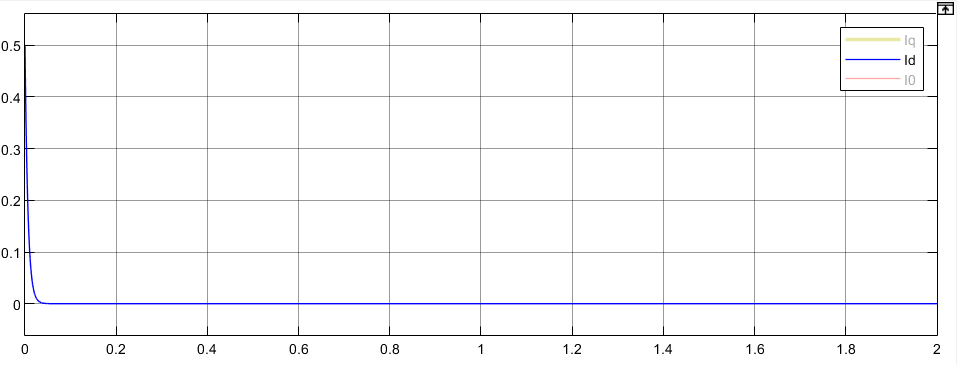
\includegraphics[width=0.8\textwidth]{5.1.6_cid1.png}
        \caption{Respuesta de la corriente en el eje $d$ ($i_d(t)$) en función del tiempo para la condición inicial $i^r_{ds}(0) = 0.5 A$.}
    \end{figure}

    \item $i^r_{ds}(0) = -0.5 A$
    
    \begin{figure}[H]
        \centering
        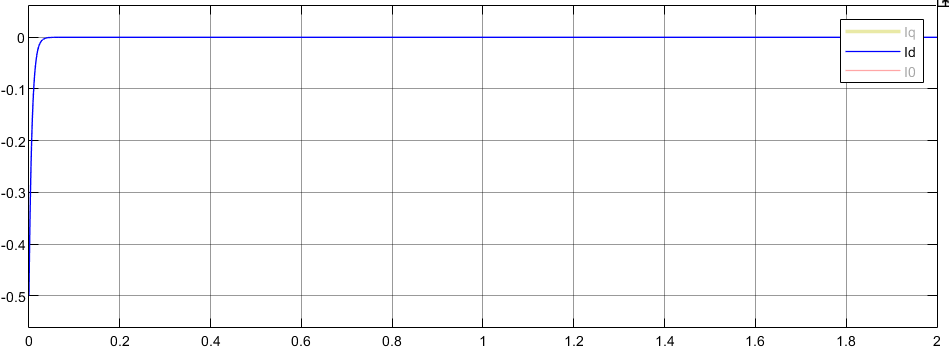
\includegraphics[width=0.8\textwidth]{5.1.6_cid2.png}
        \caption{Respuesta de la corriente en el eje $d$ ($i_d(t)$) en función del tiempo para la condición inicial $i^r_{ds}(0) = -0.5 A$.}
    \end{figure}
\end{itemize}

A continuación mostramos los resultados obtenidos en el modelo "LTI equivalente aumentado".

\begin{itemize}
    \item $i^r_{ds}(0) = 0.5 A$
    
    \begin{figure}[H]
        \centering
        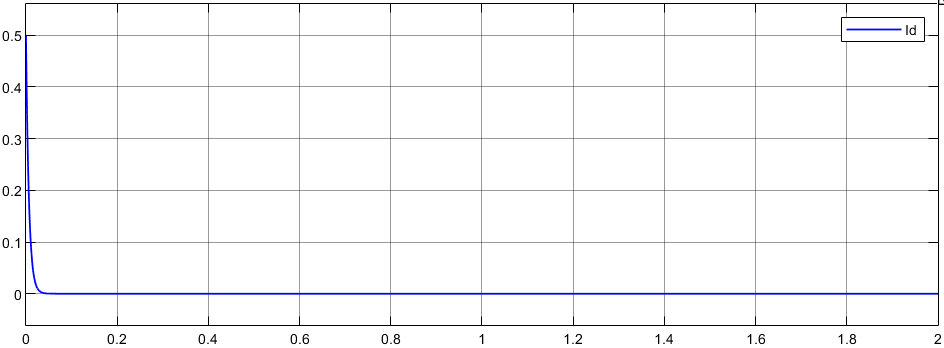
\includegraphics[width=0.8\textwidth]{5.1.6_cid3.png}
        \caption{Respuesta de la corriente en el eje $d$ ($i_d(t)$) en función del tiempo para la condición inicial $i^r_{ds}(0) = 0.5 A$.}
    \end{figure}

    \item $i^r_{ds}(0) = -0.5 A$
    
    \begin{figure}[H]
        \centering
        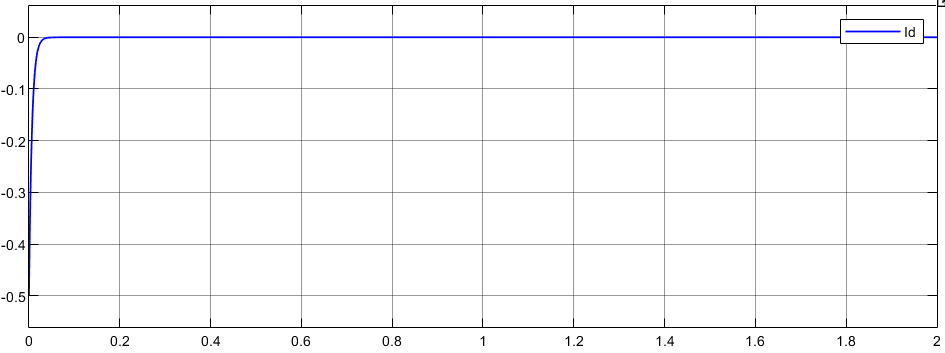
\includegraphics[width=0.8\textwidth]{5.1.6_cid4.png}
        \caption{Respuesta de la corriente en el eje $d$ ($i_d(t)$) en función del tiempo para la condición inicial $i^r_{ds}(0) = -0.5 A$.}
    \end{figure}
\end{itemize}

No se aprecian diferencias significativas en la evolución de la corriente en tiempo real entre ambos 
modelos en ninguno de los casos.

Se nota que no existen efectos notables en la evolución de las demás variables del sistema cuando se 
impone $i^r_{ds}(0) = ±0.5 \, A$. Esto se debe a que, mediante la Ley de Control complementaria mínima en el 
eje q, se elimina por completo el acoplamiento residual NL, incluso en régimen natural, logrando un 
modelo equivalente completamente lineal e independiente del estado inicial de $i^r_{ds}(t)$.

\subsubsection{Field forcing/weakening}

Añadimos una nueva consigna de tensión en el eje '$d$' a las especificaciones ya mencionadas, con el 
valor $V^r_{ds}(t) = 0 \, V \rightarrow V^r_{qs_nom}/10 = ±1,9596 \, Vcc$ en $t_{step1} = 0,5 \, s$ 
(field forcing/weakening a lazo abierto), sumada a la restricción o ley de control NL.

\begin{figure}[H]
    \centering
    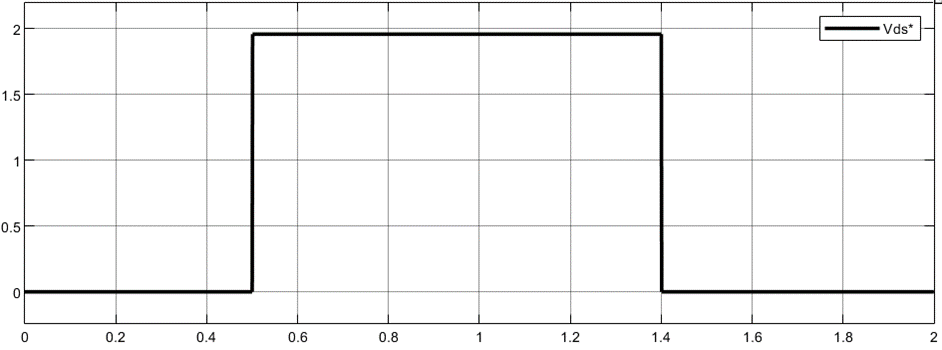
\includegraphics[width=0.8\textwidth]{5.1.6_d1.png}
    \caption{Consigna de tensión $v^*_{ds}$ para field forcing.}
\end{figure}

\begin{figure}[H]
    \centering
    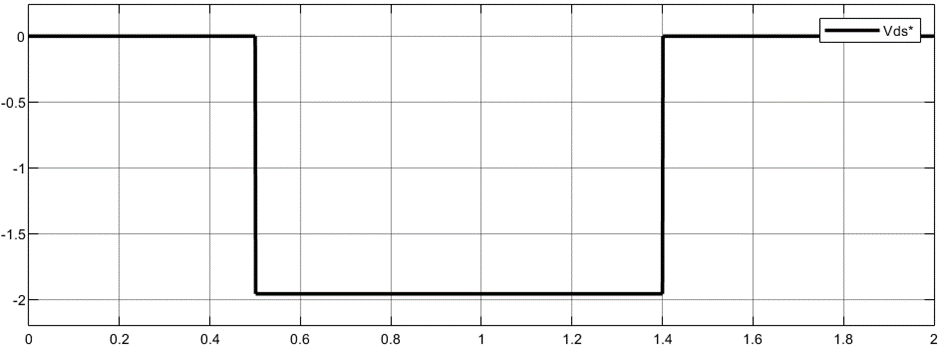
\includegraphics[width=0.8\textwidth]{5.1.6_d2.png}
    \caption{COnsigna de tensión $v^*_{ds}$ para field weakening.}
\end{figure}

\begin{figure}[H]
    \centering
    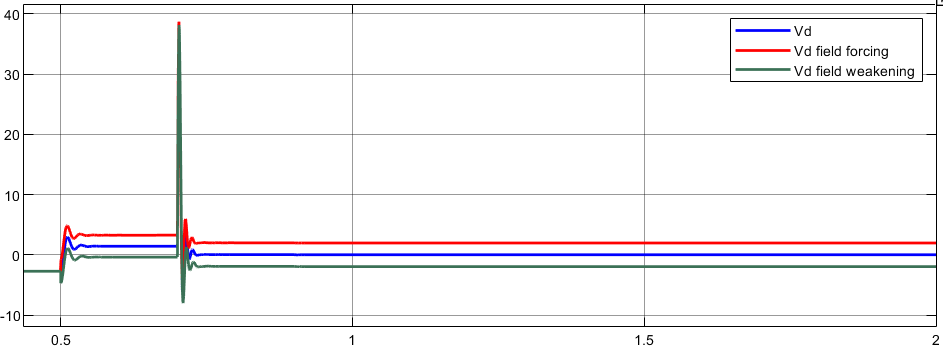
\includegraphics[width=0.8\textwidth]{5.1.6_d3.png}
    \caption{Valores finales de $v_{ds}(t)$ con consigna.}
\end{figure}

La comprobación de los efectos previamente mencionados muestra que un debilitamiento del campo 
magnético del estator (field weakening) produce un aumento en la velocidad angular en estado 
estacionario, mientras que disminuye el torque motor. Por otro lado, el reforzamiento del campo 
magnético del estator (field forcing) produce una disminución de la velocidad angular en estado 
estacionario, pero a su vez aumenta el torque motor.

\begin{figure}[H]
    \centering
    \includegraphics[width=0.8\textwidth]{5.1.6_d4.png}
    \caption{Comparación de velocidad angular para field forcing/weakening y sin ningún efecto.}
\end{figure}

\begin{figure}[H]
    \centering
    \includegraphics[width=0.8\textwidth]{5.1.6_d5.png}
    \caption{Comparación de torque electromagnético para field forcing/weakening y sin ningún efecto.}
\end{figure}

Por otro lado podemos observar los efectos de mantener esta consigna de $V_d$ en las gráficas de 
$\theta$ y $T_s$. En la primera se provoca un desfasaje en los valores finales mientras que la 
temperatura crece de manera lineal hasta que la misma cese la tensión.

\begin{figure}[H]
    \centering
    \includegraphics[width=0.8\textwidth]{5.1.6_d6.png}
    \caption{Comparación de posición angular para field forcing/weakening y sin ningún efecto.}
\end{figure}

\begin{figure}[H]
    \centering
    \includegraphics[width=0.8\textwidth]{5.1.6_d7.png}
    \caption{Comparación de temperatura del estator para field forcing/weakening y sin ningún efecto.}
\end{figure}

Es crucial señalar que esta nueva consigna no afecta en absoluto al sistema LTI equivalente aumentado. 
La razón radica en el hecho de haber desacoplado la corriente en directo de la corriente en 
cuadratura, lo que implica la pérdida de la posibilidad de realizar este tipo de acciones

\newpage

%-------------------- 5.2 --------------------------%


\section{Diseño, análisis y simulación con controlador de movimiento en cascada con modulador de torque equivalente (Control Vectorial)}

El control vectorial es una técnica avanzada que se emplea en la gestión de máquinas eléctricas, como 
los motores de corriente alterna y las máquinas síncronas. Esta metodología posibilita el control 
independiente de la magnitud y la fase de la corriente de alimentación de la máquina, permitiendo así 
un control preciso del torque y la velocidad. Una implementación frecuente de este tipo de control es 
el controlador de movimiento en cascada con modulador de torque equivalente, especialmente en aplicaciones 
de alto rendimiento como los sistemas de tracción eléctrica y los sistemas de accionamiento de maquinaria 
industrial.

En el esquema del controlador de movimiento en cascada con modulador de torque equivalente, se utiliza 
un controlador de velocidad externo para generar una señal de referencia de velocidad. Esta señal se 
compara con la velocidad real de la máquina eléctrica, y la diferencia entre ambas señales se utiliza 
para generar una señal de referencia de torque. Este sistema es fundamental para controlar la corriente 
de alimentación de la máquina. Posteriormente, el modulador de torque equivalente se emplea para 
transformar la señal de referencia de torque en una señal de corriente de alimentación que se aplica 
a la máquina.

%-------------------- 5.2.1 --------------------------%

\subsection{Modulador de torque equivalente (Controlador interno vectorial de corriente/torque)}

En su funcionamiento, el Modulador de Torque Equivalente recibe consignas de torque como entradas, 
que representan la cantidad de par motor deseado. Estas consignas de torque se convierten posteriormente 
en consignas de tensión, lo que permite controlar la magnitud y la fase de la corriente de alimentación 
de la máquina eléctrica de forma independiente.

%-------------------- 5.2.1.a --------------------------%

\subsubsection{Desacople de las realimentaciones de estado hacia la entrada}

Es posible lograr el desacoplamiento de todas las realimentaciones físicas naturales de 
estado hacia la entrada en una máquina eléctrica mediante la implementación de una estrategia 
de control adecuada que utilice un modulador de tensión con ganancia unitaria. Para esto debemos 
suponer que el modulador de tensión es lo suficientemente rápido y preciso, de forma que no 
introduzca una amplificación o atenuación adicional de la señal. 

Con esta hipótesis podemos considerar que la consigna de tensión a seguir en entrada del modulador 
de tensión sera la misma que se aplicara en la salida. Est ose pude expresar como: 

\begin{equation}
    v_{abc}(t) \approx v^*_{abc}(t)
\end{equation}

Como ya vimos anteriormente, podemos pasar de coordenadas $abc$ a coordenadas $dq0$ mediante la
transformada de Park. Por lo tanto, podemos expresar la consigna de tensión en coordenadas $dq0$


Utilizando la transformada de Park, podemos definir una consigna de tensión en coordenadas virtuales 
$v^{r*}_{qd0s}(t)$ que nos permita obtener una tensión $v^{r}_{qd0s}(t)$ que compense los efectos de 
retroalimentación y permita el desacople de las variables de estado.

Recordando las \hyperref[eq:mi_ecuacion]{Ecuaciones \ref*{eq:mi_ecuacion}}, se observa que los términos 
del lado derecho de la igualdad, a excepción de las tensiones de fase virtuales, representan las 
realimentaciones físicas del sistema. Por lo tanto, podemos definir las compensaciones que deben 
realizarse en el controlador para cancelar los efectos de la retroalimentación, las cuales son:

\begin{equation}\label{eq:compensaciones}
    \begin{cases}
        v^r_{qs}(t) = v^{r*}_{qs}(t) + R_{s}.i_{qs}^r(t) + \omega_m(t).P_p.[\lambda^{\prime r}_m + L_d.i_{qs}^r(t)] \\
        v^r_{ds}(t) = v^{r*}_{ds}(t) + R_{s}.i_{ds}^r(t) - \omega_m(t).P_p.L_q.i_{qs}^r(t) \\
        v^r_{0s}(t) = v^{r*}_{0s}(t) + R_{s}.i_{0s}^r(t) \\
    \end{cases}
\end{equation}

Realizando estas compensaciones, tenemos acceso directo a manipular el torque electromagnético, 
sin los efectos de las realimentaciones físicas, ni las caídas de tensión en los bobinados.

Reemplazando las \hyperref[eq:compensaciones]{Ecuaciones \ref*{eq:compensaciones}} en las
\hyperref[eq:mi_ecuacion]{Ecuaciones \ref*{eq:mi_ecuacion}}, se obtienen las siguientes expresiones:

\begin{equation}\label{eq:proporcionlaidad_corrientes_tensiones_de_entrada}
    \begin{cases}
        v^{r*}_{qs}(t) = L_q. \dot{i}_{qs}^r(t) \\
        v^{r*}_{ds}(t) = L_d. \dot{i}_{ds}^r(t) \\
        v^{r*}_{0s}(t) = L_{ls}. \dot{i}_{0s}^r(t) \\
    \end{cases}
\end{equation}

A continuación mostramos los diagramas de bloques: 

\begin{figure}[H]
    \centering
    \includegraphics[width=0.8\textwidth]{desacople_expandido.png}
    \caption{Diagrama de bloques de realimentación y desacople de variables.}
\end{figure}

\begin{figure}[H]
    \centering
    \includegraphics[width=0.25\textwidth]{desacople.png}
    \caption{Diagrama de bloques de realimentación y desacople de variables compacto.}
\end{figure}

%-------------------- 5.2.1.b --------------------------%

\subsubsection{Diseño de lazos de control de corrientes}

La consigna de tensión es función de la corriente del sistema, por lo que se puede controlar usando 
una consigna de corriente proporcional. Con el error de corriente entre la corriente de consigna 
$i_{qd0s}^{r*}(t)$y la corriente real del sistema se modela $v_{qd0s}^{r*}(t)$ con una ley de 
control proporcional.. El modelo resultante es el siguiente:

\begin{equation}
    \begin{cases}
        L_q. \dot{i}_{qs}^r(t) = v^{r*}_{qs}(t) = [i_{qs}^{r*}(t) - i_{qs}^r(t)].R_q^\prime \\
        L_d. \dot{i}_{ds}^r(t) = v^{r*}_{ds}(t) = [i_{ds}^{r*}(t) - i_{ds}^r(t)].R_d^\prime \\
        L_{ls}. \dot{i}_{0s}^r(t) = v^{r*}_{0s}(t) = [i_{0s}^{r*}(t) - i_{0s}^r(t)].R_{0}^\prime \\
    \end{cases}
\end{equation}

Las variables $R^\prime$ representan las ganancias del control proporcional. Se necesita obtener 
el valor de óptimo de esta ganancia, por lo cual se analiza la función de transferencia del modulador.

Al aplicar la transformada de Laplace obtenemos:

\begin{equation}
    \begin{cases}
        L_q. s.I_{qs}^r(s) = [I_{qs}^{r*}(s) - I_{qs}^r(s)].R_q^\prime \\
        L_d. s.I_{ds}^r(s) = [I_{ds}^{r*}(s) - I_{ds}^r(s)].R_d^\prime \\
        L_{ls}. s.I_{0s}^r(s) = [I_{0s}^{r*}(s) - I_{0s}^r(s)].R_{0}^\prime \\
    \end{cases}
\end{equation}

Las funciones de transferencia son:

\begin{align*}
    G_{qs}(s) &= \frac{I_{qs}^r(s)}{I_{qs}^{r*}(s)} = \frac{1}{\frac{L_q}{R_q^\prime}.s + 1}  \\
    G_{ds}(s) &= \frac{I_{ds}^r(s)}{I_{ds}^{r*}(s)} = \frac{1}{\frac{L_d}{R_d^\prime}.s + 1}  \\
    G_{0s}(s) &= \frac{I_{0s}^r(s)}{I_{0s}^{r*}(s)} = \frac{1}{\frac{L_{ls}}{R_{0}^\prime}.s + 1}
\end{align*}

Se puede observar que las funciones de transferencia son de primer orden y no poseen ceros. Dado que
los parámetros son positivos también podemos afirmar que las funciones de transferencia son estables.

Estas funciones de transferencia tienen la forma típica de un filtro pasa bajos, donde el valor que
multiplica a la variable $s$ es la constante del tiempo del sistema \tau que a la vez es el inverso
la frecuencia de corte del filtro. Si \tau toma un valor muy pequeño, dispondremos de una ancho de 
banda muy grande, lo cual proporciona una respuesta rápida.

El polo del filtro pasa bajos es $p = -\frac{1}{\tau}$ y dado que para todos los lazos $p = -5000 rad/s$
podemos calcular los valores de las ganancias:

\begin{equation}
    \frac{L}{R^\prime} = -\frac{1}{p} \to R^\prime = -L.p
\end{equation}

Resolviendo para cada rama:

\begin{align*}
    R_q^\prime &= -L_q.p = 29\varOmega  \\
    R_d^\prime &= -L_d.p = 33\varOmega \\
    R_0^\prime &= -L_{ls}.p = 4\varOmega
\end{align*}

Con este lazo de corriente logramos que el error entre la consigna de corriente y la corriente real
converja mas rápidamente a cero, de forma que responda de mejor manera a las perturbaciones.

\begin{figure}[H]
    \centering
    \includegraphics[width=0.8\textwidth]{modulador_de_corriente_extendido.png}
    \caption{Diagrama de bloques de modulador de corriente expandido.}
\end{figure}

\begin{figure}[H]
    \centering
    \includegraphics[width=0.25\textwidth]{modulador_de_corriente.png}
    \caption{Diagrama de bloques de modulador de corriente.}
\end{figure}

%-------------------- 5.2.1.c --------------------------%

\subsubsection{Incorporación de consigna de torque}

Volvemos a usar nuevamente el método de la sección anterior en el que realizamos una realimentación
para controlar el sistema mediante consignas de torque $T_m^*(t)$. La consigna sigue el siguiente modelo:

\begin{equation}
    T_m^*(t) = T_m^{r\prime}(t) + b_{eq}.\omega_m(t)
\end{equation}

Este modelo contempla la realimentación física debida a la fricción, que genera perdidas en el torque.

Sabiendo que el torque y la corriente están relacionados por la ecuación del
\hyperref[eq.torque_electromagnetico]{Torque electromagnético (\ref*{eq.torque_electromagnetico})}
expresamos las consignas de troque $T_m^{*\prime}$ en función de las consignas de corriente $i_{qs}^{r*}$:

\begin{equation}
    T_m^{*}(t) = \frac{3}{2}.P_p.[\lambda_m^{\prime r} + (L_d - L_q)i_{ds}^{r}(t)].i_{qs}^{r*}(t)
\end{equation}

Despejando de estas ultimas dos ecuaciones, obtenemos:

\begin{equation}
    i_{qs}^{r*}(t) = \frac{T_m^{*\prime}(t) + b_{eq}.\omega_m(t)}{\frac{2}{3}.P_p.[\lambda_m^{\prime r} + (L_d - L_q)i_{ds}^{r}(t)]}
\end{equation}

% IMAGEN DEL MODULADOR DE TORQUE %

\begin{figure}[H]
    \centering
    \includegraphics[width=0.8\textwidth]{modulador_de_torque_expandido.png}
    \caption{Diagrama de bloques de modulador de torque expandido.}
\end{figure}

\begin{figure}[H]
    \centering
    \includegraphics[width=0.25\textwidth]{modulador_de_torque.png}
    \caption{Diagrama de bloques de modulador de torque.}
\end{figure}

% DUDAS YA QUE NO TRABAJAMOS CON IDS %

De esta ecuación podemos determinar el efecto que tendrá la corriente $i_{ds}^{r*}$ sobre el flujo magnético:

\begin{itemize}
    \item Si $i_{ds}^{r*} > 0 A$ entonces se produce un reforzamiento de campo.
    \item Si $i_{ds}^{r*} = 0 A$ entonces se produce un desacople entre la rama correspondiente a 
    la cuadratura que anula los efectos de reforzamiento y debilitamiento.
    \item Si $i_{ds}^{r*} < 0 A$ entonces se produce un debilitamiento de campo.
\end{itemize}

%-------------------- 5.2.2 --------------------------%

\subsection{Controlador externo de movimiento (posición/velocidad)}

El controlador externo de movimiento se agrega con el fin de mejorar la dinámica del sistema y corregir los
errores de estado estacionario producidos por cargas perturbadoras. En la rama derivativa tomaremos el 
error entre la consigna de velocidad y la velocidad real. El error de posición se obtiene integrando el 
error de velocidad lo que indica que no son variables independientes, este va en la rama proporcional.
En la rama integral se tendrá la integral del erro de posición. 

% Filtro pasa alto %
Con esta configuración del controlador PID solo tendremos como entrada el error de velocidades, no tendremos
que introducir acciones derivativas lo que nos permitirá evitar la amplificación del ruido y obtener un 
controlador mas estable. Los bloques integrales actúan como filtros pasa bajos lo que nos ayuda a eliminar
el ruido de los errores de posición y velocidad dada su naturaleza de alta frecuencia.

Se diseña el controlador utilizando el método de sintonía serie con $n = 2,5$, $\omega_{pos} = 800 rad/s$, y
considerando los valores nominales de $j_l$, $b_l$. 

El controlador de movimiento se muestra en la siguiente figura: 

% IMAGEN DEL PID %

La salida del controlador sera el torque consigna que ingresara al modulador de torque. Modelando en el 
dominio de Laplace se tiene:

\begin{equation}\label{eq.controlador_error}
    T_m^{*\prime}(s) = e_\omega(s).b_a + e_\theta(s).K_{sa} + e_\theta(s).K_{sai}.\frac{1}{s}
\end{equation}

Donde:

\begin{align*}
    e_\theta(s) &= \Theta_m^*(s) - \Theta_m(s) \\
    e_\omega(s) &= e_\theta(s).s
\end{align*}

La relación entre el torque y la variación de velocidad del motor en el modelo del subsistema mecánico, 
teniendo en cuanta el desacople de fricción realizado anteriormente, es:

\begin{equation}
    J_{eq}.\dot{\omega}_(t) = T_m^*(t) - \frac{T_l(t)}{r}
\end{equation}

Aplicando la transformada de Laplace:

\begin{equation}
    J_{eq}.s^2.\Theta_m(s) = T_m^*(s) - \frac{T_l(s)}{r}
\end{equation}

Reemplazando esta ecuación en la
\hyperref[eq.controlador_error]{ecuación del controlador (\ref*{eq.controlador_error})}:

\begin{equation}
    J_{eq}.s^3.\Theta_m(s) = [s^2.b_a + s.K_{sa} + K_{sai}].[\Theta_m^*(s) - \Theta_m(s)] - s.\frac{T_l(s)}{r}
\end{equation}

Despejando, la posición del retor queda expresada como:

\begin{equation}
    \Theta_m(s) = \frac{s^2.b_a + s.K_{sa} + K_{sai}}{s^3.J_{eq} + s^2.b_a + s.K_{sa} + K_{sai}}.\Theta_m^*(s) - \frac{s}{s^3.J_{eq} + s^2.b_a + s.K_{sa} + K_{sai}}.\frac{T_l(s)}{r}
\end{equation}

A partir de esta ecuación podemos obtener las funciones de transferencia del controlador:

\begin{align}
    G_1(s) &= \frac{\Theta_m(s)}{\Theta_m^*(s)} = \frac{s^2.b_a + s.K_{sa} + K_{sai}}{s^3.J_{eq} + s^2.b_a + s.K_{sa} + K_{sai}} \\
    G_2(s) &= \frac{\Theta_m(s)}{\frac{T_l(s)}{r}} = -\frac{s}{s^3.J_{eq} + s^2.b_a + s.K_{sa} + K_{sai}}
\end{align}

En régimen estacionario para una entrada escalón unitario podemos observar:

\begin{itemize}
    \item $K_{sai} \neq 0 \to G_1(s) = 1 $ y $G_2(s) = 0$
    \item $K_{sai} = 0 \to G_2(s) = 1 $ y $G_2(s) = \frac{1}{K_{sa}} $
\end{itemize}

Estos resultados muestran que que la función de transferencia
correspondiente a la entrada de perturbación tejen un cero en el origen por lo que el error de estado 
estacionario es nulo. En caso de que la acción integral sea nula si tendrá un error dado por $1/K_{sa}$.
En cuanto a la función de transferencia correspondiente a la entrada de referencia tiene ganancia
unitaria a baja frecuencia por lo que el error de estado estacionario, según el teorema del valor final, 
es nulo. Podemos concluir que este  controlador no tiene error de régimen permanente ante entradas del tipo escalón.

Aplicamos el método de sintonía en serie, con $n = 2,5$ y $\omega_{pos} = 800 rad/s$
para la determinar las ganancias del controlador. Dado que el polinomio 
característico de forma normalizada del sistema es:

\begin{equation}
    P(s) = s^3 + \frac{b_a}{J_{eq}}.s^2 + \frac{K_{sa}}{J_{eq}}.s + \frac{K_{sai}}{J_{eq}}
\end{equation}

Podemos llegar a las siguientes expresiones:

\begin{align*}
    n.\omega_{pos} &= \frac{b_a}{J_{eq}}; & &n.\omega_{pos}^2 = \frac{K_{sa}}{J_{eq}}; & n.\omega_{pos}^3 = \frac{K_{sai}}{J_{eq}} \\
\end{align*}

Dados los valores nominales de $J_{eq}$ y $b_l$, se obtiene $J_{eq} = 5,6510.10^6$, entonces:

\begin{align*}
    b_a = J_{eq}.n.\omega_{pos} &= 0,0113\, \frac{N.m}{rad/s} \\ 
    K_{sa} = J_{eq}.n.\omega_{pos}^2 &= 9,0416\, \frac{N.m}{rad} \\
    K_{sai} = J_{eq}.n.\omega_{pos}^3 &= 2893\, \frac{N.m}{rad.s}
\end{align*}

Con estos valores podemos determinar los polos del sistema a lazo cerrado. Sabiendo que la distancia
de los polos al origen es la misma para los 3 polos. Con $\xi = 0,75$

\begin{itemize}
    \item Para valores nominales de $J_l$ y $b_l$:
    
    \begin{align*}
        s_1 = -800\, \frac{rad}{s} & & s_2,3  = -600 \pm 529,15\, j \, \frac{rad}{s} 
    \end{align*}
    
    \item Para valores máximos de $J_l$ y $b_l$:
    
    \begin{align*}
        s_1 = -613,75\, \frac{rad}{s} & & s_2,3  = -508,98 \pm 649,26\, j \, \frac{rad}{s} 
    \end{align*}

    \item Para valores mínimos de $J_l$ y $b_l$:
    
    \begin{align*}
        s_1 = -1498,5\, \frac{rad}{s} & & s_2,3  = -542,3 \pm 383,7\, j \, \frac{rad}{s} 
    \end{align*}

\end{itemize}

% MOSTRAR LA IMAGEN DE LOS POLOS %

%-------------------- 5.2.2 --------------------------%

\subsubsection{Entrada de referencia o set-point}

Por último, se incluye la opción de ingresar el control de posición mediante una referencia o punto de 
ajuste de posición de las coordenadas articulares del brazo del robot SCARA. Esto resulta conveniente, ya que 
en muchas ocasiones es más sencillo utilizar los algoritmos de Cinemática del robot para controlar 
el brazo, utilizando sus coordenadas articulares. De forma que:

\begin{equation}
    q_1^* = \frac{\theta_m^*(t)}{r}
\end{equation}

% IMAGEN DEL SET-POINT %

%-------------------- 5.2.3 --------------------------%

\subsection{Observador de Estado de orden reducido}

Un observador de estado es un componente utilizado en sistemas de control para estimar el estado interno 
de un sistema dinámico a partir de las mediciones de entradas y salidas del sistema. En este caso, se
utiliza un observador de estado de orden reducido para poder realimentar la velocidad angular del motor 
ya que este no cuenta con un sensor para medirla directamente.

El sistema no es observable desde la velocidad $\omega_m(t)$ como lo indica el criterio de observabilidad 
de Kalman, pero si desde la posición $\theta_m(t)$. Por lo tanto estimaremos la velocidad a partir de la 
posición.

Al incorporar el observador al subsistema mecánico podemos omitir $-b_{eq}.\omega_{m}(t)$ ya que al 
contar con sensores de corriente con realimentación física este efecto ya está desacoplado.  

El modelo del subsistema mecánico se puede expresar como:

\begin{equation}
    \begin{cases}
        \dot{x}(t) = A.x(t) + B_c.u(t) +B_d.d(t)  \, ; \,\, x(t_0) = x_0\\
        y(t) = C.x(t) \\
    \end{cases}
\end{equation}

\begin{equation}
    \begin{cases}
        \dot{x}(t) = 
        \begin{bmatrix}
            0 & 1 \\
            0 & 0 \\
        \end{bmatrix}
        .x(t) + 
        \begin{bmatrix}
            0 \\
            \frac{1}{J_{eq}} \\
        \end{bmatrix}
        .T_m(t) +
        \begin{bmatrix}
            0 \\
            -\frac{1}{J_{eq}.r} \\
        \end{bmatrix}
        .T_l(t)\\
        y(t) = 
        \begin{bmatrix}
            1 & 0 \\
        \end{bmatrix}
        .x(t) \\
    \end{cases}
\end{equation}

El observador de estado de Luenberger crea un modelo estimado del sistema original que reproduce su 
comportamiento a partir de las variables de entrada y salida medibles. Luego, utiliza este modelo estimado 
junto con una corrección proporcional al error de salida para estimar el estado interno del sistema en 
tiempo real. Aplicándolo al sistema anterior, se obtiene:

\begin{equation}
    \begin{cases}
        \dot{\hat{x}}(t) = \hat{A}.\hat{x}(t) + \hat{B}.u(t) + K_e.(y(t) - \hat{y}(t)) \, ; \,\, \hat{x}(t_0) = 0\\
        \hat{y}(t) = \hat{C}.\hat{x}(t) \\
    \end{cases}
\end{equation}

Donde la matriz $K_e$ contiene los parámetros de ajuste del observador

\begin{equation}
    K_e = 
    \begin{bmatrix}
        k_{e\theta} & k_{e\omega} \\
    \end{bmatrix}
\end{equation}

Con el error de estimación definido como:

\begin{equation}\label{eq.error_estimacion}
    e(t) = x(t) - \hat{x}(t)
\end{equation}

Asumiendo un funcionamiento ideal, las matrices de ambos sistemas real coinciden con las matrices del
modelo del observador. Trabajando el sistema y reemplazando en la   
\hyperref[eq.error_estimacion]{ecuación (\ref*{eq.error_estimacion})}
se obtiene la dinámica del error:

\begin{equation}
    \dot{e}(t) = [A - K_e.C].e(t) + B.d(t)
\end{equation}

Considerando que no hay perturbaciones $d(t) = 0$, se pueden obtener los parámetros de ajuste del observador
mediante el polinomio característico del sistema dado por los autovalores de la matriz 
$A^\prime = [A - K_e.C]$:

\begin{equation}
    \mid s.I - A^\prime\mid \,\,= 
    \begin{bmatrix}
        s + k_{e\theta} & -1 \\
        k_{e\omega} & s 
    \end{bmatrix}
    = s^2 + k_{e\theta}.s + k_{e\omega}
\end{equation}

Resolviendo el polinomio y sabiendo que los polos son $p_{1,2} = -3200\, rad/s$, obtengo:

\begin{align*}
    K_{e\theta} = 6400\,rad/s \\
    K_{e\omega} = 10,24.10^6\,rad/s
\end{align*}

% IMAGEN DEL OBSERVADOR %

%-------------------- 5.2.4 --------------------------%

\subsection{Simulación en tiempo continuo con modelo completo NL}

\subsubsection{Seguimiento de consignas de movimiento}

La posición deseada de la articulación, $q^*_1(t)$, se define como una función de tiempo que depende 
de la variable $θ^∗_m(t)$, donde $r$ es una constante. 

Para generar el perfil de movimiento, utilizamos un perfil trapezoidal en el que tanto la rampa de 
ascenso como la de descenso se producen en un intervalo de tiempo de 5 segundos. Durante este tiempo,
la posición deseada de $q^∗_1(t)$ alcanza un valor de $2\pi$ radianes entre las dos rampas.

\begin{figure}[H]
    \centering
    \includegraphics[width=1\textwidth]{perfil_trapezoidal.png}
\end{figure}

\begin{figure}[H]
    \centering
    \includegraphics[width=1\textwidth]{5.2.4.a.2.png}
\end{figure}

\begin{figure}[H]
    \centering
    \includegraphics[width=1\textwidth]{5.2.4.a.3.png}
\end{figure}

\begin{figure}[H]
    \centering
    \includegraphics[width=1\textwidth]{5.2.4.a.4.png}
\end{figure}

\begin{figure}[H]
    \centering
    \includegraphics[width=1\textwidth]{5.2.4.a.5.png}
\end{figure}

\begin{figure}[H]
    \centering
    \includegraphics[width=1\textwidth]{5.2.4.a.6.png}
\end{figure}

\subsubsection{Rechazo a perturbaciones}

para evaluar la respuesta del sistema ante perturbaciones, proporcionamos una consigna constante 
igual a 0 con un escalón como perturbación.

\begin{figure}[H]
    \centering
    \includegraphics[width=1\textwidth]{5.2.4.b.1.png}
\end{figure}

\begin{figure}[H]
    \centering
    \includegraphics[width=1\textwidth]{5.2.4.b.2.png}
\end{figure}

Notamos un error de estado estacionario en este caso.

\begin{figure}[H]
    \centering
    \includegraphics[width=1\textwidth]{5.2.4.b.3.png}
\end{figure}

%-------------------- 5.2.5 --------------------------%

\subsection{Verificación de desempeño y/o mejoras}

%-------------------- 5.2.5.a --------------------------%

\subsubsection{Especificaciones de operación (valores límites)}

\begin{center}
    \begin{tabular}{|c|c|c|c|c|}
        \hline
         & \multicolumn{2}{c|}{Especificación de Operación} & \multicolumn{2}{c|}{Valores obtenidos en simulación} \\
        \hline
         & Régimen continuo & Valor máximo & Régimen continuo & Valor máximo \\
        \hline
        Torque motor & 0.023 & 0.093 & 0.009 & 3.7 \\
        \hline
        Velocidad angular & 691.15 &  & 394.9 &  \\
        \hline
        Corriente en el estator & 0.4 & 2 & 0.030 & 54 \\
        \hline
        Tensión en el estator & 24 &  & 19.01 &\\
        \hline
    \end{tabular}
\end{center}

Causa primera: puntos de inflexión en la consigna genera picos muy altos.

Una forma de mejorar esto es suavizar la consigna. Podemos aplicar un filtro a la entrada de esta 
o como en nuestro caso, trabajar sobre el perfil de velocidad angular. Al eliminar los cambios 
abruptos o líneas verticales, logramos eliminar los picos que se generan en los puntos de 
inflexión del perfil de posición.

\begin{figure}[H]
    \centering
    \includegraphics[width=1\textwidth]{5.2..5.1.a.1.png}
\end{figure}

\begin{figure}[H]
    \centering
    \includegraphics[width=1\textwidth]{5.2..5.1.a.2.png}
\end{figure}

\begin{figure}[H]
    \centering
    \includegraphics[width=1\textwidth]{5.2..5.1.a.3.png}
\end{figure}

\begin{figure}[H]
    \centering
    \includegraphics[width=1\textwidth]{5.2..5.1.a.4.png}
\end{figure}

\begin{figure}[H]
    \centering
    \includegraphics[width=1\textwidth]{5.2..5.1.a.5.png}
\end{figure}

Al aplicar este cambio hacemos que el sistema no sobrepase los valores pico de las especificaciones
que eran los que no respondían de forma satisfactoria.

%-------------------- 5.2.5.b --------------------------%

\subsubsection{Observador}

En las simulaciones que hemos realizado, se puede observar un error de estado estacionario no nulo 
ante perturbaciones de carga. Este error surge debido a que el observador de estado no está 
realimentando la entrada de perturbación. Aunque podría ser tentador tratar de corregir esto 
mediante la realimentación del par de carga, esto podría implicar la adición de sensores costosos 
y potencialmente imprecisos, lo que mantendría el error.

En lugar de esto, proponemos una solución a través de la adición de una acción integral al 
observador de estado, un enfoque que aborda el problema a través de software sin requerir hardware 
adicional. Esto implica la introducción de un nuevo estado en nuestro observador que tiene en 
cuenta el tiempo que permanece la estimación del estado en un valor erróneo. Este nuevo estado es 
una integración del error entre la variable medida y su estimación, y se define como:

\begin{equation}
    z(t) = \int (\theta(t) - \hat{\theta}(t))\,dt
\end{equation}

Ahora, el modelo del observador se redefine para incluir este estado integral y la entrada del 
observador también se ajusta para incluir este nuevo estado:

\begin{align*}
    \dot{\tilde{\theta}}(t) &= K_e \theta \left(\theta(t) - \tilde{\theta}(t)\right) + \tilde{\omega}(t) \\
    \dot{\tilde{\omega}}(t) &= K_e \omega \left(\theta(t) - \tilde{\theta}(t)\right) + T_m \dot{'}(t) J_eq + z(t) \\
    \dot{\tilde{z}}(t) &= K_e i \left(\theta(t) - \tilde{\theta}(t)\right)
\end{align*}

Para sintonizar las ganancias del observador, determinamos la ecuación característica del 
observador y la comparamos con la de un sistema con características deseadas. Para este propósito, 
asumimos que queremos que todos los polos del observador estén ubicados en -3200 rad/s. Esto nos 
da los valores de las ganancias del observador:

\begin{align*}
    K_e\theta = 9.6 \times 10^3 \, \text{rad/s}
    K_e\omega = 3.072 \times 10^7 \, \text{rad/s}^2
    K_ei = 3.2768 \times 10^{10} \, \text{rad/s}^3
\end{align*}

Estas ganancias aseguran que el error de estado estacionario converja asintóticamente a cero, 
incluso ante perturbaciones de carga. Así, la adición de la acción integral en el observador ha 
resuelto el problema sin la necesidad de hardware adicional.

\begin{figure}[H]
    \centering
    \includegraphics[width=1\textwidth]{5.2.5.1.b.1.png}
\end{figure}

Vemos como el valor de tita real es igual a 0 luego de un transitorio debido a la perturbación. 
Esto además se puede corroborar en la siguiente imagen que representa el error entre la consigna y 
el valor real de la posición angular:

\begin{figure}[H]
    \centering
    \includegraphics[width=1\textwidth]{5.2.5.1.b.2.png}
\end{figure}

%-------------------- 5.2.5.c --------------------------%

\subsubsection{Comportamiento térmico del motor}

Procedemos a verificar la temperatura del bobinado cuando la consigna involucra una operación 
continua repetitiva sumado una perturbación continua. Estas dos se crearon a partir de la consigna 
inicial repetida dentro de un lapso de $300$ segundos.

\begin{figure}[H]
    \centering
    \includegraphics[width=1\textwidth]{5.2.5.1.c.1.png}
    \caption{Temperatura sin suavizado}
\end{figure}

Vemos que cuando la consigna es la original, el sistema sobrepasa los limites de temperatura, lo 
que podría producir una degradación de los componentes. Además notamos que esta se vuelve 
asintótica.
    
\begin{figure}[H]
    \centering
    \includegraphics[width=1\textwidth]{5.2.5.1.c.2.png}
    \caption{Temperatura con suavizado}
\end{figure}
    
En este caso, al igual que en el anterior, la respuesta en temperatura se vuelve asintótica pero 
a valores dentro de los limites permitidos.

%-------------------- 5.2.5.d --------------------------%

\subsubsection{Desempeño del sistema ante una respuesta no ideal de los sensores}

En este segmento, se estudian los efectos de las respuestas no ideales (banda limitada) de los 
sensores que miden las corrientes, la posición angular del motor, y la temperatura. Se siguen las 
siguientes especificaciones:

\begin{itemize}
    \item Sensor de corriente: modelo pasa bajo (LP) en el espacio de estados (SS) de 2° orden, 
    con una frecuencia natural de $6000\,rad/s$ y un factor de amortiguamiento $(\xi)$ de $1$.

    \item Sensor de posición angular: modelo LP en SS de 2° orden, con una frecuencia natural de 
    $2000\,rad/s$ y un factor de amortiguamiento de $1$.

    \item Sensor de temperatura: modelo LP en SS de 1° orden, con una constante de tiempo ($\tau$)  
    de $20\,s$.
\end{itemize}

Para los filtros de segundo orden, se usa la función de transferencia:

\begin{equation*}
    G(s) = \frac{\omega_n^2}{s^2 + 2\omega_n\zeta s + \omega_n^2}
\end{equation*}

Donde se puede demostrar que la función de transferencia de un modelo en el espacio de estados se 
calcula con la ecuación:

\begin{equation*}
    G(s) = C(sI - A)^{-1}B + D
\end{equation*}

Si se toma como matriz de estados $A$:

\[
A = \begin{bmatrix}
0 & -1 \\
\omega_n^2 & -2\omega_n\zeta
\end{bmatrix}
\]

Entonces, igualando las ecuaciones, las matrices del modelo en el espacio de estados deben ser:

\[
A = \begin{bmatrix}
0 & -1 \\
\omega_n^2 & -2\omega_n\zeta
\end{bmatrix}, \quad
B = \begin{bmatrix}
1 \\
0
\end{bmatrix}, \quad
C = \begin{bmatrix}
0 & 1
\end{bmatrix}, \quad
D = \begin{bmatrix}
0
\end{bmatrix}
\]

Por lo tanto, los sensores de corriente y posición angular quedan definidos por:

Para el sensor de corriente:

\[
A_{iac} = \begin{bmatrix}
0 & -1 \\
36 \times 10^6 & -12000
\end{bmatrix}, \quad
B_{iac} = \begin{bmatrix}
1 \\
0
\end{bmatrix}, \quad
C_{iac} = \begin{bmatrix}
0 & 1
\end{bmatrix}, \quad
D_{iac} = \begin{bmatrix}
0
\end{bmatrix}
\]

Para el sensor de posición:
\[
A_{pos} = \begin{bmatrix}
0 & -1 \\
4 \times 10^6 & -4000
\end{bmatrix}, \quad
B_{pos} = \begin{bmatrix}
1 \\
0
\end{bmatrix}, \quad
C_{pos} = \begin{bmatrix}
0 & 1
\end{bmatrix}, \quad
D_{pos} = \begin{bmatrix}
0
\end{bmatrix}
\]

Para el filtro de primer orden, la función de transferencia es:

\[
G(s) = \frac{1}{1 + \tau s}
\]

De donde se puede deducir que:

Para el sensor de temperatura:
\[
A_T = \begin{bmatrix}
-0.05
\end{bmatrix}, \quad
B_T = \begin{bmatrix}
1
\end{bmatrix}, \quad
C_T = \begin{bmatrix}
0.05
\end{bmatrix}, \quad
D_T = \begin{bmatrix}
0
\end{bmatrix}
\]

\begin{figure}[H]
    \centering
    \includegraphics[width=1\textwidth]{5.2.5.d.1.png}
\end{figure}

\begin{figure}[H]
    \centering
    \includegraphics[width=1\textwidth]{5.2.5.d.2.png}
\end{figure}

\begin{figure}[H]
    \centering
    \includegraphics[width=1\textwidth]{5.2.5.d.3.png}
\end{figure}

\begin{figure}[H]
    \centering
    \includegraphics[width=1\textwidth]{5.2.5.d.4.png}
\end{figure}

\begin{figure}[H]
    \centering
    \includegraphics[width=1\textwidth]{5.2.5.d.5.png}
\end{figure}

\begin{figure}[H]
    \centering
    \includegraphics[width=1\textwidth]{5.2.5.d.6.png}
\end{figure}

\begin{figure}[H]
    \centering
    \includegraphics[width=1\textwidth]{5.2.5.d.7.png}
\end{figure}

\begin{figure}[H]
    \centering
    \includegraphics[width=1\textwidth]{5.2.5.d.8.png}
\end{figure}

\begin{figure}[H]
    \centering
    \includegraphics[width=1\textwidth]{5.2.5.d.9.png}
\end{figure}

\begin{figure}[H]
    \centering
    \includegraphics[width=1\textwidth]{5.2.5.d.10.png}
\end{figure}

\begin{figure}[H]
    \centering
    \includegraphics[width=1\textwidth]{5.2.5.d.11.png}
\end{figure}

\begin{figure}[H]
    \centering
    \includegraphics[width=1\textwidth]{5.2.5.d.12.png}
\end{figure}

\begin{figure}[H]
    \centering
    \includegraphics[width=1\textwidth]{5.2.5.d.13.png}
\end{figure}

\begin{figure}[H]
    \centering
    \includegraphics[width=1\textwidth]{5.2.5.d.14.png}
\end{figure}

\begin{figure}[H]
    \centering
    \includegraphics[width=1\textwidth]{5.2.5.d.15.png}
\end{figure}

\begin{figure}[H]
    \centering
    \includegraphics[width=1\textwidth]{5.2.5.d.16.png}
\end{figure}

%-------------------- 5.2.5.d --------------------------%

\subsubsection{Moduladore trifásico de tensión no ideal}

El desempeño de un sistema eléctrico se analiza incorporando características no ideales en el 
modulador de tensión trifásico, centrando la atención en la saturación y limitación del ancho de 
banda. Se modela el modulador como un filtro pasa bajos con una saturación de tensión definida por 
$√2.V_s.√3$, donde $V_{smáx} = 24\,Vca$ rms. El filtro pasa bajo se define con una frecuencia 
natural $\omega = 6000\,rad/s$ y un factor de amortiguamiento $\xi = 1$, representándose en el 
espacio de estados con las siguientes matrices: 

    \begin{align*}
    A = \begin{bmatrix}
    0 & -1 \\
    36 \times 10^6 & -12000
    \end{bmatrix}, \quad
    B = \begin{bmatrix}
    10
    \end{bmatrix}, \quad
    C = \begin{bmatrix}
    0 & 1
    \end{bmatrix}, \quad
    D = \begin{bmatrix}
    0
    \end{bmatrix}
\end{align*}

Estas matrices provienen de las obtenidas en el punto anterior. 

Al implementar estas características no ideales, se observa una degradación en el desempeño 
del sistema. La saturación del modulador provoca un creciente error entre la consigna y la
posición actual. Este error se debe a que la máquina no recibe la tensión necesaria para generar 
el torque correcto y corregir su posición. En consecuencia, las tensiones reales se estancan en 
sus valores límites de saturación, mientras que las consignas de tensión siguen aumentando de 
forma exponencial. 

Por otro lado, la introducción del modelo de filtro pasa-bajo provoca efectos 
similares a la degradación de los sensores. La solución sugerida para estas inestabilidades es la 
incorporación de la dinámica de los sensores y el modulador de torque en el modelo del sistema, 
lo que permitiría un ajuste más preciso

Aplicando inicialmente solo la saturación:

\begin{figure}[H]
    \centering
    \includegraphics[width=1\textwidth]{5.2.5.e.1.png}
\end{figure}

\begin{figure}[H]
    \centering
    \includegraphics[width=1\textwidth]{5.2.5.e.2.png}
\end{figure}

Notamos que no afecta significativamente ya que para alcanzar la consigna suavizada, las tensiones 
nunca superan la de saturación.

Continuamos la simulación aplicando los bloques necesarios para implementar una respuesta no ideal 
del modulador, ante la consigna con la que venimos trabajando. Se obtuvieron los siguientes 
resultados:

\begin{figure}[H]
    \centering
    \includegraphics[width=1\textwidth]{5.2.5.e.3.png}
\end{figure}

\begin{figure}[H]
    \centering
    \includegraphics[width=1\textwidth]{5.2.5.e.4.png}
\end{figure}

Vemos que ahora el sistema es incapaz de cumplir con la consigna.

%-------------------- 5.2.6 --------------------------%

\subsection{Version Final}

\begin{figure}[H]
    \centering
    \includegraphics[width=1\textwidth]{5.2.6.png}
\end{figure}

\newpage

\part*{Conclusiones}

Al final podemos llegar a concluir...

\newpage

\part*{Referencias}

A continuación se listan las referencias utilizadas para la realización de este trabajo:


\label{LastPage}    

\end{document}